%\documentclass{article}
%\usepackage[utf8]{inputenc}

%\title{Frontmatter}
%\author{wcc.weichihchen }
%\date{May 2021}

%\begin{document}

%\maketitle


%\end{document}



\documentclass[12pt,letterpaper,oneside,draft]{book}
\usepackage[tmargin=1in,bmargin=1in,lmargin=1.5in,rmargin=1in,footskip=0.25in]{geometry}


\usepackage{lipsum}
\usepackage{amsmath}

\usepackage{fancyhdr}
\pagestyle{fancy}
\fancyhf{}
\fancyheadoffset{0cm}
\renewcommand{\headrulewidth}{0pt} 
\renewcommand{\footrulewidth}{0pt}


\usepackage{setspace}
\doublespacing

% For table of contents %

% Redefinition of ToC command to get centered heading
\usepackage{tocloft}
\renewcommand{\cftdotsep}{1}
\renewcommand{\contentsname}{\hspace*{\fill} {TABLE OF CONTENTS} \hspace*{\fill}}
%\renewcommand{\contentsname}{\hfill { } \hfill}
\renewcommand{\cfttoctitlefont}{\mdseries}
\renewcommand{\cftbeforetoctitleskip}{-72pt}
\renewcommand{\cftaftertoctitleskip}{52pt} 
%\renewcommand{\cftchapfont}{}
\renewcommand{\cftpartfont}{\normalfont}
\renewcommand{\cftpartpagefont}{\normalfont}
\renewcommand{\cftchapfont}{\normalfont}
\renewcommand{\cftchappagefont}{\normalfont}

\renewcommand{\cftsecfont}{\normalfont}
\renewcommand{\cftsecpagefont}{\normalfont}

\renewcommand{\cftsubsecfont}{\normalfont}
\renewcommand{\cftsubsecpagefont}{\normalfont}

\renewcommand{\cftpartleader}{\cftdotfill{\cftdotsep}} % dots for parts
\renewcommand{\cftchapleader}{\cftdotfill{\cftdotsep}} % dots for chapters
\renewcommand\cftpartafterpnum{\vspace{-24pt}}

%%%%%%%%%% LIST OF TABLES %%%%%%%%%%
\renewcommand{\listtablename}{\hfill LIST OF TABLES \hfill} 

\renewcommand\cftlottitlefont{\mdseries}
\renewcommand\cfttabfont{\normalfont}
\renewcommand\cfttabpagefont{\normalfont}


\renewcommand{\cftlottitlefont}{{~}\hfill\normalfont}
\renewcommand{\cftafterlottitle}{%
\hfill{~}\\[\baselineskip]{\vspace{-36pt}\normalfont\textit{
Table}}\hspace{372pt}{\normalfont\textit{ Page}}}


\setlength{\cftafterlottitleskip}{40pt}
\setlength{\cfttabindent}{8pt}


%%%%%%%%%% LIST OF FIGURES %%%%%%%%%%
\renewcommand{\listfigurename}{\hfill LIST OF FIGURES \hfill}

\renewcommand\cftloftitlefont{\mdseries}
\renewcommand\cftfigfont{\normalfont}
\renewcommand\cftfigpagefont{\normalfont}


\renewcommand{\cftloftitlefont}{{~}\hfill\normalfont}
\renewcommand{\cftafterloftitle}{%
\hfill{~}\\[\baselineskip]{\vspace{-36pt}\normalfont\textit{
Figure}}\hspace{368pt}{\normalfont\textit{ Page}}}
\setlength{\cftafterloftitleskip}{40pt}
\setlength{\cftfigindent}{8pt}

%%%%%%%%%% LIST OF ABBREVIATIONS %%%%%%%%%%
%\usepackage[nopostdot,style=longtable,nonumberlist]{glossaries}


%\loadglsentries{abbreviations.tex}
%\makeglossaries
%%%%%%%%%% REFERENCES %%%%%%%%%%

\usepackage{natbib}

\setlength\bibsep{12pt}
\newcommand\mybibname{\hfill { } \hfill}
\renewcommand\bibsection{%
    \setlength\bibhang{2in}
    \noindent\normalsize\MakeUppercase{\mybibname}%
    \markboth{\MakeUppercase{\mybibname}}{\MakeUppercase{\mybibname}}%
  }


%%%%%%%%%%%%%%%%%%%%%%%%%%%%%%%%
%%%%%%%%%%%%%%%%%%%%%%%%%%%%%%%%
%%%%%%%%%%%%%%%%%%%%%%%%%%%%%%%%
\usepackage{gensymb}

\usepackage[final]{graphicx}% Include figure files
%\usepackage{graphicx}% Include figure files
\usepackage{hyperref}% add hypertext capabilities
\usepackage[font=normal,format=plain,labelfont=bf,up,textfont=normal,up]{caption} % for the alignment of caption


\begin{document}
	\newgeometry{tmargin=2in,bmargin=1in,lmargin=1.5in,rmargin=1in}
	% Cover
	\frontmatter
    \begin{singlespace}
	{\centering
		PREDICTIVE MODELING OF SUPERHARD AND TOPOLOGICAL MATERIALS BY DENSITY FUNCTIONAL THEORY AND MACHINE LEARNING\par
	}
	\vskip 72pt
	{\centering
		by \par
	}
	\vskip 12pt
	{\centering
		WEI-CHIH CHEN
	\par
	}
	\vskip 24pt
	{\centering
		CHENG-CHIEN CHEN, COMMITTEE CHAIR
	\par
	}

	{\centering
		KANNATASSEN APPAVOO
	\par
	}
	{\centering
		ILIAS E. PERAKIS
	\par
	}
	{\centering
		YOGESH K. VOHRA
	\par
	}
	{\centering
		MARY ELLEN ZVANUT
	\par
	}
	%\vspace{2.4in}%{180pt}%{2.5in}
	\vspace{204pt}%{2.5in}
	{\centering
		A DISSERTATION
	\par
	}
	\vskip 12pt
	{\centering
		Submitted to the graduate faculty of The University of Alabama at Birmingham,\\
		in partial fulfillment of the requirements for the degree of\\ 
		Doctor of Philosophy
	\par
	}
	\vskip 12pt
	{\centering
		BIRMINGHAM, ALABAMA
	\par
	}
	\vskip 12pt		
	{\centering
		2021
	\par
	}
    \end{singlespace}
    
	% Copyright

	\newgeometry{tmargin=680pt,bmargin=1in,lmargin=1.5in,rmargin=1in}

    \begin{singlespace}
	{\centering
		Copyright by\\
		Wei-Chih Chen\\
		2021\par
	}
    \end{singlespace}
	\restoregeometry
	% Abstract
	\addcontentsline{toc}{part}{ABSTRACT} 
	\pagestyle{plain} % this line would give you
	                      % small roman numeral page number
		{\centering
		\singlespacing
			PREDICTIVE MODELING OF SUPERHARD AND TOPOLOGICAL MATERIALS BY DENSITY FUNCTIONAL THEORY AND MACHINE LEARNING\par
		}
		\vskip 12pt
		{\centering
			WEI-CHIH CHEN\par
		}
		\vskip 12pt
		{\centering
			PHYSICS\par
		}
		\vskip 12pt
		{\centering
			ABSTRACT\par
		}
		\vskip 12pt
%%%%%%%%%% ABSTRACT %%%%%%%%%%
        In this dissertation, we focus on the computational prediction for new superhard materials and topological phase transitions in quantum materials. To search for new superhard materials, we employed machine learning techniques, evolutionary crystal structure prediction, and density functional theory to explore new superhard materials in ternary B-C-N and B-N-O compounds. For the B-C-N systems, our machine learning prediction shows that a 1:1 B-N ratio can lead to various superhard compositions. Our subsequent evolutionary algorithm searches indicated that BC$_{10}$N has an extremely high hardness $\sim$ 87 GPa based on density functional theory. For B-N-O systems, we adopted an self-improvement computational procedure, and found that ternary compounds with a chemical formula B$_{x+2}$N$_{x}$O$_{3}$ (e.g. B$_5$N$_3$O$_3$, B$_6$N$_4$O$_3$, etc) are thermodynamically favorable, and several superhard B-N-O compounds can be found when $x \geq 3$. Our studies for new ternary superhard materials show that machine learning is a powerful tool to accelerate material discovery.

		In our studies for topological materials, we found that ZrTe$_5$ is in the vicinity of topological phase transition. By means of the uniaxial tensile strain, ZrTe$_5$ undergoes a $Z_2$ transition from a strong topological insulator phase to a weak topological insulator phase. In the case of LaN, we found that LaN has a low-temperature, ferroelectric phase with $P1$ symmetry, and it would undergo a structural phase transition to rock-salt phase ($Fm\bar{3}m$ symmetry) when the temperature is increased. Besides, a hydrostatic pressure $\sim$ 18 GPa can lead to a structural phase transition to tetragonal structure ($P4/nmm$ symmetry). Our topological studies show that high-temperature rock-salt LaN can change from a topologically trivial phase to a topologically non-trivial phase at $P$ $\sim$ 14 GPa, and its topological phase transition can also be induced by the temperature at a pressure between 14 and 18 GPa. These results show that strain engineering and hydrostatic pressure can effectively drive topological phase transition in quantum materials.

		
		
		\pagebreak
	% Dedication
	\addcontentsline{toc}{part}{DEDICATION} 
	\newgeometry{tmargin=2in,bmargin=1in,lmargin=1.5in,rmargin=1in}
		{\centering
		\singlespacing
			DEDICATION\par
		}
		\vskip 2in
		{\centering
		
		    \textit{To God, Tao, and Nature,}
		    
		    \textit{The absolute, omnipresent, and eternal Existence}
		    
		    \vskip 0.5in
		    
		    \textit{To my parents, for their endless love and support}

		}
		\restoregeometry
		
	% Acknowledgement
	\addcontentsline{toc}{part}{ACKNOWLEDGEMENT}
	\newgeometry{tmargin=2in,bmargin=1in,lmargin=1.5in,rmargin=1in}
		{\centering
		\singlespacing
			ACKNOWLEDGEMENT\par
		}
		\vskip 48pt
%%%%%%%%% ACKNOWLEDGEMENT %%%%%%%%%%
        Throughout my PhD period, I have received many helps from many people, and this dissertation would not be possible without their efforts, time, and insights. First, wholeheartedly I appreciate my advisor, Dr. Cheng-Chien Chen, who always provides guidance and support for my cultivation of scientific literacy. Especially, I thank Dr. Chen for the detailed instructions on large-scale many-body calculations, machine learning applications, and scientific writings.
        
        This period as an graduate student would be much more difficult without the supports of fellowships. I want to show my biggest appreciation for the support by Dr. Cheng-Chien Chen, Dr. Ilias E. Perakis, and Dr. Mary Ellen Zvanut for their recommendations for UAB Blazer Graduate Research Fellowship. Besides, I thank Dr. Cheng-Chien Chen again and Dr. Yogesh K. Vohra for their supports for CPU2AL Graduate Research Assistantships.
        
        There are many research collaborators that I have worked with during these years. I thank Dr. Yogesh K. Vohra, Dr. Shane Aaron Catledge, Dr. Paul Baker, Kallol Chakrabarty, and Kaleb Burrage in UAB for their experiments on high hardness materials. I also thank Dr. Jiun-Haw Chu and Joshua Mutch in University of Washington for ZrTe$_5$ synthesis and measurements. I also appreciate Dr. Yao Wang in Clemson University for the collaboration and discussion on extended Hubbard model. Besides, I appreciate Dr. Joseph Maciejko in University of Alberta for the discussion of topological materials. In the end, I would like to appreciate my classmate and friend Chia-Min Lin for his company throughout my PhD period.
    \restoregeometry
    \pagebreak
	
	%%%%%%%%%% TABLE OF CONTENTS PAGE %%%%%%%%%%
	
	{\centering
		\vspace{0pt} \hspace{0pt} \par
	}
	{\centering
		\vspace{1in} \hspace{0pt} \par
	}
	\hspace*{\fill} \textit{Page}



    \tableofcontents
	\pagebreak

	%%%%%%%%%% LIST OF TABLES PAGE %%%%%%%%%%
    
    \addcontentsline{toc}{part}{LIST OF TABLES}
    \listoftables
    \pagebreak
	%%%%%%%%%% LIST OF FIGURES PAGE %%%%%%%%%%

    \addcontentsline{toc}{part}{LIST OF FIGURES}
    \listoffigures
    \pagebreak
	%%%%%%%%%% LIST OF ABBREVIATIONS PAGE %%%%%%%%%%
%    \printglossary[type=\acronymtype,nonumberlist,title=\normalfont \normalsize \protect\centering LIST OF ABBREVIATIONS]
    
    %\printglossary[type=main]
%    \addcontentsline{toc}{part}{LIST OF ABBREVIATIONS}
%    \pagebreak
    

%    \restoregeometry
%    \addtocontents{toc}{\protect\renewcommand{\protect\cftsecleader}{\hfill}}

%%%%%%%%%%%%%%%%%%%%%%%%%%%%%%%%%%%%%%%%%%%%%%%%%%
%%%%%%%%%%%%%%%%%%%%%%%%%%%%%%%%%%%%%%%%%%%%%%%%%%

    \cftaddtitleline{toc}{chap}{\vspace{26pt}CHAPTER\vspace{-16pt}}{}
    

%%%%%%%%%%%%%%%%%%%%%%%%%%%%%%%%%%%%%%%%%%%%%%%%%%
%%%%%%%%%%%%%%%% main text starts %%%%%%%%%%%%%%%%
%%%%%%%%%%%%%%%%%%%%%%%%%%%%%%%%%%%%%%%%%%%%%%%%%%

	\mainmatter 
	%\fancyhead[R]{\thepage}
	\pagestyle{plain}{
		\fancyhf{}
		\fancyhead[R]{\thepage}
	}
	

    %\chapter{1 INTRODUCTION}
    \newcounter{numch}  % counter for chapter
    \addtocounter{numch}{1}
    
    \addcontentsline{toc}{chapter}{\hspace{4pt}  \the\value{numch} \hspace{4pt} INTRODUCTION}
    
	{\centering
		\vspace{0pt} \hspace{0pt} \par
	}
	{\centering
		\vspace{56pt} CHAPTER  \the\value{numch}
	}
	{\centering\singlespacing
		INTRODUCTION
	    \par
	}
	{\centering
		\vspace{0pt} \hspace{0pt} \par
	}
    Searching for materials with desired properties and controlling functional quantum materials are always central objectives of materials science and condensed matter physics. Traditional materials science research relies on experiments including sample synthesis, characterization, and optimization, which are usually time-consuming and economically expensive. With the advances of quantum-mechanical theories for the many-body problem and efficient algorithms, first-principles calculations have reached reasonable accuracy and have become important tools allowing us to design and study materials before doing experiments. Among methods used to solve the many body problem, density functional theory (DFT) can render several accurate ground state properties, and therefore has been widely used in theoretical studies. Besides, the constantly increasing computer power and the development of efficient DFT codes have facilitated high-throughput screening. The huge amount of data then make machine learning possible to accelerate the material discovery.
    
    In this work, we first focus on searching for new ternary superhard materials including B-C-N and B-N-O compounds. Our studies include DFT calculations, machine learning methods, and crystal structure prediction by the evolutionary algorithm. Another focus of this dissertation is topological materials with quantum spin Hall effect, which are known to host exotic surface states. In particular, we have studied the topological phase transitions in zirconium pentatelluride and lanthanum monopnictides by means of strain engineering and hydrostatic pressure, respectively. In the following, we introduce superhard materials and topological materials.
    
    %\subsection*{Summary of Superhard Materials}
    \addcontentsline{toc}{subsection}{Summary of Superhard Materials}
	{\centering
		\vspace{12pt}Summary of Superhard Materials
	    \par
	}

Hardness is the property that quantifies a material's resistance to plastic deformation. Today, there are three main hardness measurements: scratch, indentation, and rebound. In the studies of superhard materials, the Vickers indentation is the most-used measurement to determine the hardness. The indenter in Vickers hardness test is a piece of diamond in a shape of a pyramid, which has an angle of 136$^\circ$ between two adjacent faces. During the measurement, a load is applied to the sample, and an indentation mark would be left on the sample. The value of Vickers hardness ($H_V$), with an unit of pressure, can be calculated by $F/A$, where $F$ is the applied force and $A$ is the area of indentation. In practice, one can determine the value of $H_V$ by
	\begin{equation}
		\begin{aligned}
		\label{eq}
			H_V = 1854.4\frac{F}{d^2}.
		\end{aligned}
	\end{equation}
If $F$ is in Newton, and $d$, the average length of two diagonals, is in $\mu$m , then $H_V$ has an unit in GPa. It is important to note that for a piece of material, the value of $H_V$ depends on the applied load, and $H_V$ decreases with an increasing load in an asymptotic way. Generally, superhardness in experiments can be attributed to intrinsic effect and extrinsic effect \cite{vepvrek1999search}. The intrinsic effect relies on the compositional elements, strengths of chemical bonds, and underlying crystal structure (eg. $sp^3$-bonded diamond and cubic boron nitride). On the other hand, extrinsic effect depends on the appearance like the surface morphology, microstructures, and grain size (e.g. aggregated diamond~\cite{dubrovinskaia2005aggregated}). Here, we only focus on the intrinsic effect in high hardness materials. In the following, we introduce superhard materials as well as materials with smaller hardness but showing potential for applications in the industry.

Superhard materials are materials with a $H_V$ greater than 40 GPa~\cite{kaner2005designing}. They are of great interest with applications like drilling, grinding, cutting, and protective coatings. Their extraordinary properties make them essential in manufacturing, automotive, and petrochemical industries~\cite{zhao2016recent}. Diamond is the hardest material ($H_V$ $\sim$ 90 - 100 GPa \cite{xu2015ultrahardness}) in the world, and it also has the largest bulk modulus and shear modulus among the known materials. The superior mechanical properties of diamond are the results of its $sp^3$-bonded structure and high valence electron density. However, to fulfill different industrial needs, other properties like thermal stability, chemical stability, and fracture toughness are also important factors that affect the performance of a material \cite{monteiro2013cubic}. Diamond suffers from low oxidation temperature $\sim$ 700 $^{\circ}$C, and being reactive with ferrous materials~\cite{haines2001synthesis}, which limits its applications on steel and cast iron in heavy industry. 
    
    \begin{figure}[t]
        \centering
        \captionsetup{singlelinecheck = false, justification=justified}
        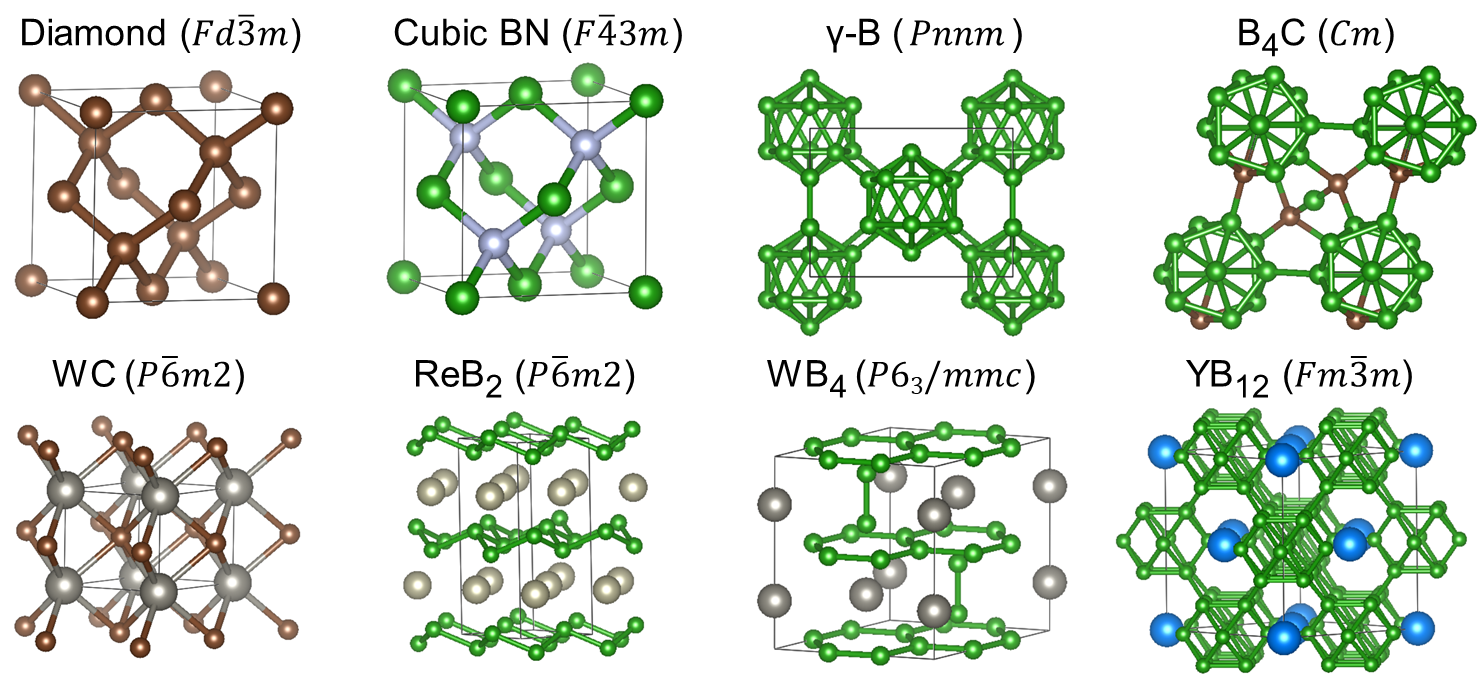
\includegraphics[width=0.95\textwidth]{selected_crystals.png}
        \caption[Crystal structures of materials with high hardness.]{Crystal structures of high-hardness materials. The corresponding space groups are shown in the parentheses.}
        \label{fig:1}
    \end{figure}

Cubic boron nitride (c-BN), with the same atomic arrangement as diamond (see Fig. \ref{fig:1}), is the second hardest material ($H_V$ $\sim$ 50 – 65 GPa) with the advantages of high thermal stability ($\sim$1300 °C) \cite{yu2006thermal,cBN_65_GPa_liu2019hardness} and being inert in contact with ferrous materials, and thereby has a complementary relationship with diamond~\cite{monteiro2013cubic}. However, its synthesis, similar to diamond, usually requires high pressure and high temperature (HPHT), which takes a great amount of energy and makes it difficult for large-scale production~\cite{zhao2016recent}. Other compounds not as hard but widely used in the industry include
cemented carbides~\cite{sun2020review,wu2013understanding}, boron-rich materials~\cite{kovziridze2013improvement,sairam2012development,jiao2010synthesis}, SiC~\cite{sung1996carbon}, and Al$_2$O$_3$~\cite{acchar2005tem}. These materials can be easily synthesized on a large-scale through processes like sintering, hot-pressing, and ball-milling. The  crystal structures of selected high hardness materials are shown in Fig. \ref{fig:1}, and the hardness comparison can be found in Fig. \ref{fig:2}.

    \begin{figure}[t]
        \centering
        \captionsetup{singlelinecheck = false, justification=justified}
        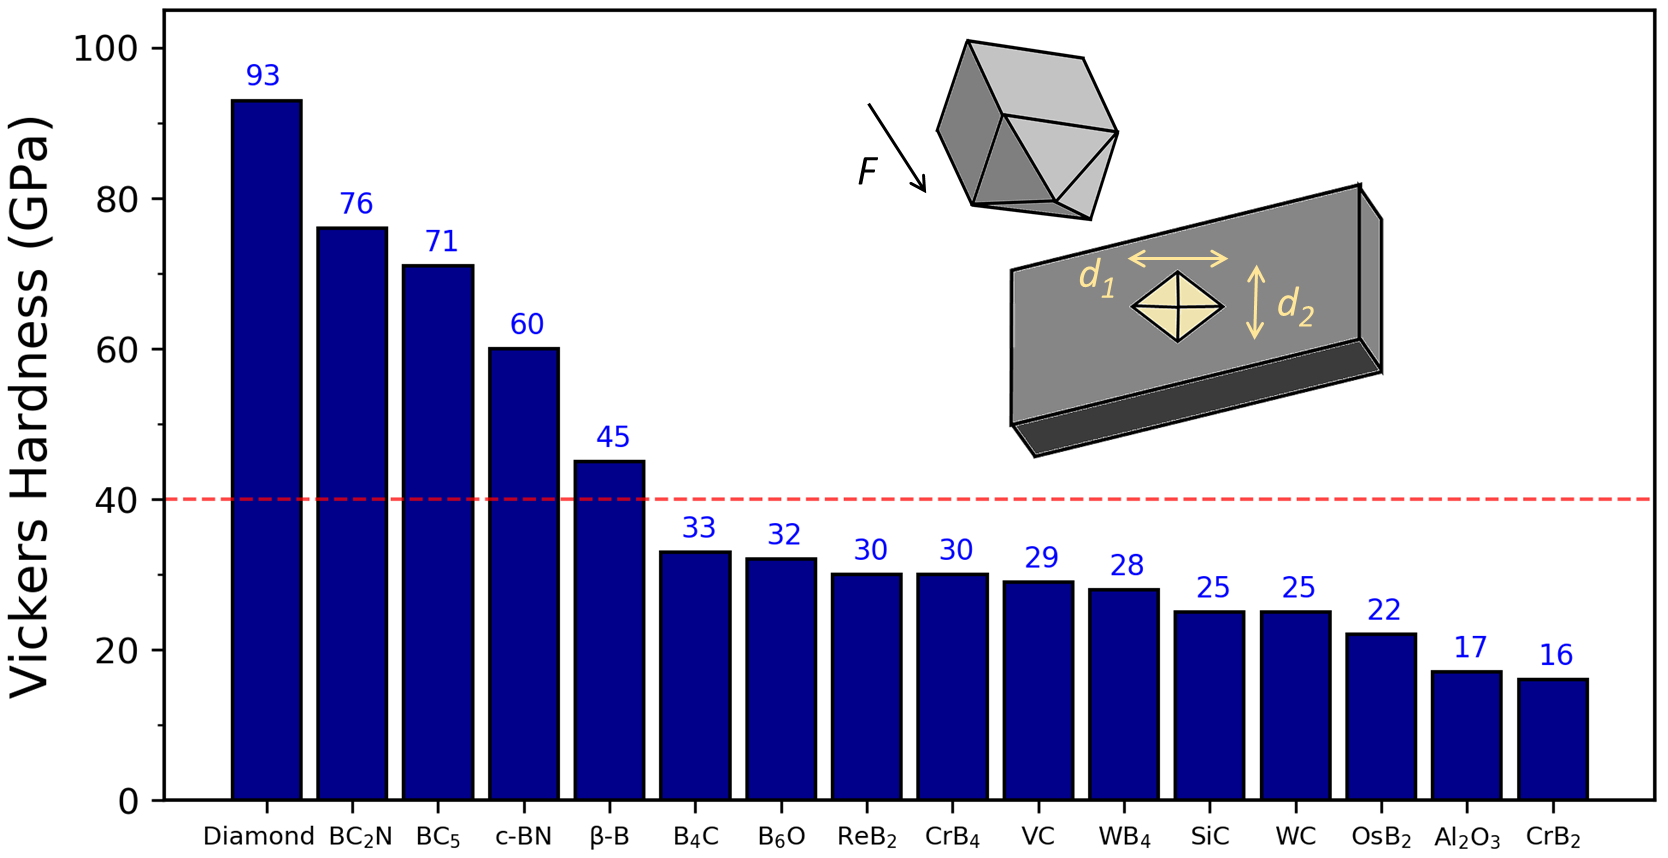
\includegraphics[width=1.0\textwidth]{superhard_materials.png}
        \caption[Vickers hardnesses of selected hard materials]{Vickers hardnesses of selected hard materials under a load $F$ $\geq$ 4.9 N.}
        \label{fig:2}
    \end{figure}


Boron and boron-rich materials with B$_{12}$ icosahedra as building blocks also have exceedingly high hardness. For elemental boron, there are three major allotropes worth noting: $\alpha$-rhombohedral boron ($\alpha$-B$_{12}$), $\beta$-rhombohedral boron ($\beta$-B$_{106}$), and $\gamma$-orthorhombic ($\gamma$-B$_{28}$), and they also have superhardness 42, 45, and 50 GPa, respectively ~\cite{solozhenko2008hardness}. Boron-rich materials like B$_4$C and B$_6$O have $\alpha$-B$_{12}$-like crystal structures with carbon or oxygen atoms sit at sites between icosahedra. They were reported to have smaller hardnesses around 35 GPa ~\cite{kovziridze2013improvement, sairam2012development, jiao2010synthesis}. Other boron-very-rich materials crystalized in tetragonal form like B$_{50}$C$_2$ and B$_{50}$N$_2$ have high hardnesses like B$_4$C \cite{baker2020first}. Besides, a recent study by Chakrabarty {\it et al.} showed that the hardness of amorphous B$_{50}$C$_2$ can be as hard as c-BN \cite{chakrabarty2020superhard}.

Transition metal (TM) borides also have superior mechanical properties, and their preparation does not require high pressure environment. Therefore, they are ideal candidates for large-scale production. TM borides have many different crystal structures ranging from monoborides (e.g. WB, CrB), diborides (e.g. ZrB$_2$, ReB$_2$), tetraborides (e.g. WB$_4$, CrB$_4$), dodecaborides (e.g. ZrB$_{12}$, YB$_{12}$) to higher borides (e.g. YB$_{50}$, YB$_{66}$). Monoborides like WB and CrB have relatively small hardness $\sim$ 30 - 35 GPa under a load of 0.49 N, and their hardnesses drops to $\sim$ 20 GPa under a load of 4.9 N~\cite{WB_yeung2016superhard, CrB_han2015hardness}. In TM diborides, TiB$_2$, ZrB$_2$, and HfB$_2$ also show relatively low hardness around 20 GPa at high load~\cite{TiB2_munro2000material,ZrB2_HfB2_zapata2013mechanical}. It is worth noting that ReB$_2$ has superhardness around 45 GPa under a 0.49 N load while its hardness drops to $\sim$ 30 GPa under a 4.9 N load. For tetraborides, WB$_4$ and CrB$_4$ are superhard with their hardnesses around 44 GPa under 0.49 N, while their high load results are also around 30 GPa. At last, dodecaborides ZrB$_{12}$ and YB$_{12}$ have slightly inferior hardnesses compared with ReB$_2$, WB$_4$ and CrB$_4$. Table \ref{tab:hardness_TM_borides} shows that the experimental results of hardness tests on selected borides are summarized in.

\vspace{24pt}


	\setlength{\tabcolsep}{12pt} % Default value: 6pt
	\renewcommand{\arraystretch}{1.5} % Default value: 1
    \begin{table}[htb]
    \captionsetup{singlelinecheck = false, justification=justified}
    %\centering
    \caption[Vickers Hardnesses of selected transition metal borides]{Vickers hardnesses of selected transition metal borides}
    \label{tab:hardness_TM_borides}
    \begin{tabular*}{\textwidth}{c|c|c|c}
        Borides  & {$H_V$ (GPa) @ 0.49 N load} & $H_V$ (GPa) @ high load & Reference  \\ \hline
        %c-BN      &       & 65 @ 4.9N   & ~\cite{cBN_65_GPa_liu2019hardness} \\
        CrB       &  30   & 20 @ 4.9 N   & ~\cite{CrB_han2015hardness} \\
        WB        &  35   & 18 @ 4.9 N   &
        ~\cite{WB_yeung2016superhard} \\
        WB$_2$    &  30   & 22 @ 4.9 N   &
        ~\cite{pangilinan2018superhard} \\
        TiB$_2$   &  -    & 20 @ 5.0 N   & ~\cite{TiB2_munro2000material} \\
        ZrB$_2$   &  -    & 17 @ 9.8 N   & ~\cite{ZrB2_HfB2_zapata2013mechanical} \\
        HfB$_2$   &  -    & 20 @ 9.8 N   & ~\cite{ZrB2_HfB2_zapata2013mechanical} \\
        CrB$_2$   &  -    & 16 @ 4.9 N   & ~\cite{CrB2_CrB4_wang2014crystal} \\
        OsB$_2$   &  27   & 18 @ 4.9 N   & ~\cite{OsB2_chung2008anisotropic} \\
        ReB$_2$   & 48, 40   & 30, 29 @ 4.9 N   & ~\cite{ReB2_chung2007synthesis},~\cite{lech2016superhard} \\
        WB$_4$    &  43   & 28 @ 4.9 N   & ~\cite{WB4_mohammadi2011tungsten} \\
        CrB$_4$   &  44   & 30 @ 4.9 N   & ~\cite{CrB2_CrB4_wang2014crystal} \\  
        %CaB$_6$   &  26   & 24 @ 4.9N   & ~\cite{CaB6_xin2011properties} \\  
        ZrB$_{12}$&  42, 40   & 28, 27 @ 4.9 N   & ~\cite{YB12_akopov2019synthesis, ZrB12_ma2017ultrastrong} \\
        YB$_{12}$ &  38   & 26 @ 4.9 N   & ~\cite{YB12_akopov2019synthesis} \\
    \end{tabular*}
    \end{table}

\vspace{24pt}

With the continuous increase in the global demand of superhard materials, searching for new materials with outstanding hardness, thermal stability, and chemical stability has become an important research topic. In this field, there are two major categories. The first one focuses on hardness enhancement in TM borides by introducing one or more TM elements. This method is known as solid solution hardening, where the atomic size mismatch causes lattice distortions. Such lattice distortions effectively inhibit the dislocation, which is necessary for plastic deformation. Besides, this kind of materials are expected to have higher thermal stability due to the increase in entropy. The second one concerns finding new superhard materials composed of light elements: B, C, N, and O. These materials have short bond lengths and strong covalent bonds, which make them the primary candidates for new superhard materials. Besides, they have the advantages of being abundant in quantity and low price compared with TMs. Next, we introduce the recent developments in these two fields.


% hardness enhancement in borides
In TM bordies, forming solid solutions by introducing one or more TM elements or mixing different borides have been recognized as an effective way to enhance the hardness. In the literature, such experiments were mostly carried out by the research group led by Richard B. Kaner. For example, several experiments have been carried out based on WB$_4$, which has a pristine hardness of 43 GPa under 0.49 N. Here, we briefly summarize their findings. Mohammadi {\it et al.} found that with the addition of 1 at.\% rhenium in WB$_4$, its hardness increases to 50 GPa at 0.49 N \cite{WB4_mohammadi2011tungsten}. Besides, when 3 at.\% molybdenum is added to WB$_4$, its hardness also increases to 50 GPa at 0.49 N \cite{WB4_Mo_H_enhancement}. Besides, Akopov {\it et al.} also carried out a series of experiments by considering three different elements: Ti, Zr, and Hf. Their hardness indentation results show that WB$_4$ alloys with 8 Ti at.\%, 8 at. Zr\%, and 6 at. Hf\% reach highest hardness values of 51, 56, and 52 GPa at 0.49 N, respectively \cite{WB4_akopov2016extrinsic}, while they attributed the observed hardness enhancements to extrinsic effect due to the changes in grain morphology. Akopov {\it et al.} also reported hardness enhancements in WB$_4$ by introducing different TMs and rare-earth elements \cite{akopov2018effects}. In their experiments, seven elements (Y, Sc, Gd, Dy, Tb, Ho, and Er) were considered, and their optimum hardness values can reach as high as 46 - 50 GPa at 0.49 N.

In another two studies, Akopov {\it et al.} also investigated the hardnesses of the mixtures of ZrB$_{12}$, YB$_{12}$, ScB$_{12}$, and UB$_{12}$ \cite{YB12_akopov2019synthesis}. They found that the highest hardness values can be achieved at 1:1 ratio: Zr$_{0.5}$Y$_{0.5}$B$_{12}$, Zr$_{0.5}$Sc$_{0.5}$B$_{12}$, and Y$_{0.5}$Sc$_{0.5}$B$_{12}$, Zr$_{0.5}$U$_{0.5}$B$_{12}$ have their hardnesses around 43 - 48 GPa at 0.49 N, which are higher than those of pure diborides (28 - 42 GPa). For systems with lower boron content , tungsten monoboride, WB, has also been studied in the similar way, Yeung {\it et al.} found W$_{0.5}$Ta$_{0.5}$B becomes superhard with a hardness of 43 GPa at 0.49 N, which is a 23 \% enhancement compared with WB's 35 GPa \cite{WB_yeung2016superhard}. Pangilinan {\it et al.} studied the solid solution of WB$_2$ by adding Ta and Nb elements \cite{pangilinan2018superhard}. Their results show that when 6 at.\% Nb and 8 at.\% Ta are introduced in WB$_2$, the values of hardness become greater than 40 GPa at 0.49 N. The hardness enhancements exceed 30 \% compared with the hardness of WB$_2$ (30 GPa at 0.49 N). In the literature, people have also considered mixing icosahedron-based boride with TM diboride. Mnatsakanyan {\it et al.} synthesized a lightweight superhard B$_4$C-27wt.\%ReB$_2$ ceramic composite, which has a superhardness of 50 GPa under a load as high as 49 N, which is comparable with cubic boron nitride.  \cite{mnatsakanyan2021superhard}.

High-entropy materials are solid solutions composed of five or more elements with (nearly) even proportions. Recently, they have attracted increasing attention because these materials are promising to be thermodynamically more stable at high temperatures, and thus have potential for high-temperature applications. In the literature, researchers have found that high-entropy borides and carbides have higher values of hardness than those of simple diborides. Gild {\it et al.} fabricated a series of single-phase high-entropy TM diborides (Hf$_{0.2}$Zr$_{0.2}$Ta$_{0.2}$M$_{0.2}$Ti$_{0.2}$B$_2$; M = Nb, Mo, Cr) \cite{gild2016high}. Their results show that  high-entropy TM diborides have higher hardness (22 GPa) and improved oxidation resistance than individual diborides. Another similar study carried out by Zhang {\it et al.} reported that Hf$_{0.2}$Zr$_{0.2}$Ta$_{0.2}$Cr$_{0.2}$Ti$_{0.2}$B$_2$ has a hardness of 28 GPa at 1.96 N \cite{zhang2019dense}.

Different from borides, Sarker {\it et al.} synthesized single-phase high-entropy TM carbides with rock-salt structure (like $\beta$-WC). Their samples consist of five out of eight TMs (Hf, Nb, Mo, Ta, Ti, V, W, and Zr) and carbon \cite{sarker2018high}. Their results show that high-entropy carbides can enhance hardness up to 50 \% higher than the rule of mixtures. Besides, they also proposed the ``entropy forming ability'' as an indicator for synthesizability from first-principles calculations. In the following, we introduce the second route to find new superhard materials: ternary compounds that composed of light elements: B, C, N, and O.

% B-C-N-O compounds as new superhard materials
Similar to the studies of TM borides, mixing two compounds that composed of B, C, and N in each have been reported in the literature. In the case of elemental carbon and boron, Solozhenko {\it et al.} synthesized diamond-like BC$_5$ under HPHT, and found that the synthesized BC$_5$ has a hardness of 71 GPa \cite{PhysRevLett.102.015506}. They also reported that BC$_5$ has relatively high fracture toughness, and exceptional thermal stability (1900 K). Recently, Baker {\it et al.} used microwave plasma chemical vapor deposition (MPCVD) to synthesize boron-incorporated diamond at low temperature and low pressure, and they found the hardness can reach as high as 62 GPa in their cubic phase sample with a boron content of 7.7 at\% \cite{baker2018computational}. 

In the literature, ternary B-C-N compounds with superhardness have also been investigated by researchers. Cubic BC$_2$N, with 1:1 composition ratio of carbon and boron nitride, was reported to have superhardness of 76 or 62 GPa \cite{solozhenko2001mechanical, BC2N_solozhenko2001synthesis, BC2N_zhao2002superhard}. Not only harder than c-BN, experimental results also show that BC$_2$N remains stable up to 1800 K, which demonstrates its superior thermal stability than diamond. Other possibilities like BCN and BC$_9$N in cubic phase have also been synthesized under extreme conditions \cite{BCN_liu2011synthesis}.

Ternary B-C-O materials have also been synthesized in the experiments. Garvie {\it et al.} used HPHT techniques to synthesized B-C-O compounds, and their results show solid solutions composed of B$_4$C and B$_6$O. In particular,
B$_6$C$_{1.1}O_{0.33}$ and B$_6$C$_{1.28}$O$_{0.31}$ with $\alpha$-B$_{12}$ structure were grown \cite{hubert1997high}. Similarly, Bolotina {\it et al.} also reported synthesized BC$_{0.155}$O$_{0.155}$ under HPHT, which also has a structure like $\alpha$-B$_{12}$ \cite{bolotina2001atomic}. Reasearchers have also used computaitonal crystal structure prediction to search for superhard B-C-O compounds. B$_2$CO were studied independently by two research groups while different structures were discovered \cite{li2011b2co,liu2017superhard}. Both of them reported that B$_2$CO is possible to be superhard based on their density functional theory (DFT) calculations. Another theoretical study used particle swarm algorithm to search for new possibilities in B$_2$C$_x$O systems \cite{zhang2015influences}. Their results show that higher carbon content increases the number of $sp^3$ bonds between carbon atoms and thereby enhances the mechanical properties. They reported that B$_2$C$_3$O has a hardness of 51 - 68 GPa. Wang {\it et al.} used variable-composition evolutionary searches to study the B-C-O systems \cite{wang2016novel}. They reported several metastable structures including B$_4$CO$_4$, B$_6$C$_2$O$_5$, and B$_2$CO$_2$, and their simulated hardnesses are around 35-40 GPa suggesting that they might be superhard materials. Among them, B$_4$CO$_4$ is energetically favorable, and it becomes thermodynamically stable at 23 GPa. Hence, these B-C-O compounds have potential to for future industrial applications.

As for ternary C-N-O compounds, very limited results could be found in the literature. Steele {\it et al.} used evolutionary algorithm to study C-N-O compounds, and they found that C$_2$N$_2$O can be stabilized at 10 GPa \cite{steele2017ternary} with a high bulk modulus of 232.5 GPa. Besides, another high-pressure phase, C$_3$N$_2$O$_3$, also has a high bulk modulus of 210.5 GPa, and it also becomes thermodynamically stable at 17.3 GPa,

Ternary B-N-O compounds are also not fully-explored in the literature. Li {\it et al.} used particle swarm algorithm for hardness-driven search, where hardness is the fitness function to be maximized \cite{li2015superhard}. They reported that orthorhombic B$_3$NO is superhard with a hardness greater than 45 GPa. Experimentally, Bhat {\it et al.} first synthesized single-crystalline B-N-O compounds by mixing hexagonal boron nitride and boron trioxide under HPHT ~\cite{bhat2015high}. They reported the synthesized B$_6$N$_4$O$_3$ has a zinc-blende-like structure, and their DFT simulations also indicate that it has a high bulk modulus $\sim$ 300 GPa, which is higher than any other known oxynitride.

As discussed above, several ternary compounds composed of B, C, N, and O were studied by crystal structure prediction techniques with density functional theory. However, to explore the enormous phase space in multi-component systems needs tremendous computational time to finish. Besides, traditional methods are also limited by the number of atoms in the unit-cell. Thanks to the developments of machine learning methods, new descriptors for materials, and online materials databases, now we can take advantage of machine learning and existing data to build machine learning models, which in turn can help us predict unknown properties of a material and accelerate the discovery of new materials. In this dissertation, we use two different machine learning study procedures to search for superhard B-C-N and B-N-O materials, which will be discussed in Chapter 3, ``Machine Leaning and  Evolutionary   Discovery of Ternary Superhard Materials''.

\pagebreak
























    %\subsection*{Topological Materials}
    \addcontentsline{toc}{subsection}{Topological Materials}
	{\centering
		\vspace{12pt} Topological Materials
	    \par
	}
Topology in mathematics concerns the properties that are invariants under smooth deformation. In the context of condensed matter physics, topology of a material becomes a new kind of phase classification, which is different from traditional phase classification by Landau's theory. Therefore, in topological materials, the discrete ``topological invariants'', instead of the continuous ``order parameter'', is used to label a topological phase. 

An example of topological materials is the integer quantum Hall (IQH) effect, which was first discovered by Klaus von Klitzing {\it et al.} in 1980 \cite{Klitzing1980new}. In IQH system, the behaviors of longitudinal and transverse electrical conductivities against external magnetic field cannot be understood by symmetry-breaking. Instead, the topology of electronic structure is the underlying physics behind such quantum phase transitions. In the following, we first introduce the experimental settings and outcomes of IQH effect and how topology comes into play.

The IQH effect was initially observed in silicon-based metal-oxide-semiconductor field-effect transistor (MOSFET), which can be regarded as a two-dimensional electron gas system. When the system is subjected to low temperature and high magnetic field, the electronic structure becomes the discrete Landau levels. As the Fermi level is in the gap between two Landau levels, the longitudinal conductivity $\sigma_{xx}$ disappears and the transverse conductivity (or Hall conductivity) is quantized,
	\begin{equation}
		\label{eq:2}
		\begin{aligned}
			\sigma_{xy} = - \frac{e^2}{2\pi\hbar} C,
		\end{aligned}
	\end{equation}
where $C$ is an integer representing filled Landau levels. This result indicates that the system becomes insulating in the bulk while the edge can conduct electricity. Klaus von Klitzing was latter awarded the Nobel prize in 1985. The precision level of the quantization of $\sigma_{xy}$ has been found to be one part of a billion \cite{von2005developments}, and it does not depend on intricate details like geometry and purity of the sample. Therefore, the quantized Hall conductivity in the IQH effect is a macroscopic phenomenon that manifests its topological property. The mathematical form of the integer $C$ are first obtained by Thouless, Kohmoto, Nightingale,and den Nijs (TKNN) in 1982, where they considered a 2D non-interacting electronic system with periodic potential and an uniform magnetic field \cite{TKNN}. Using the fundamental Kubo formula for electrical conductivity, TKNN found the Hall conductivity has a form
	\begin{equation}
		\label{sigma_xy}
		\begin{aligned}
			\sigma_{xy} = \frac{-e^2}{(2\pi)^2\hbar} \sum_n^{occ} \int_{BZ}  d^2k \left( i \left\langle \frac{\partial u_{n\bf k}}{\partial k_1} \middle| \frac{\partial u_{n\bf k} }{\partial k_2} \right\rangle - \left\langle \frac{\partial u_{n\bf k}}{\partial k_2} \middle| \frac{\partial u_{n\bf k} }{\partial k_1} \right\rangle \right),
		\end{aligned}
	\end{equation}
where $u_{n\bf k}$ stands for the periodic part in Bloch wavefunction. Later, Michael Berry found the geometric phase in quantum mechanics \cite{berry1984quantal}. (But this paper was published late in 1984 because one referee lost the manuscript \cite{berry2010geometric}) In 1983, Barry Simon found the integral in TKNN expression is actually Berry curvature \cite{simon1983holonomy}. Therefore, TKNN expression can be written as:
	\begin{equation}
		\label{sigma_xy}
		\begin{aligned}
			\sigma_{xy} = \frac{-e^2}{(2\pi)^2\hbar} \sum_n^{occ} \int_{BZ} d^2k \Omega_{n,z}(\textbf{k}),
		\end{aligned}
	\end{equation}
where $\Omega_{n,z}$ is the Berry curvature. Chern-Gauss-Bonnet theorem tells us that the integral of the Berry curvature over any closed 2D manifold is quantized to be 2$\pi$ times an integer. Therefore, we know each band has its own $C_n$
	\begin{equation}
		%\label{eq}
		\begin{aligned}
			\int_{BZ} \Omega_{n,z}(\textbf{k}) d^2k = 2\pi C_n.
		\end{aligned}
	\end{equation}
In the end, the Hall conductivity is
	\begin{equation}
		%\label{eq}
		\begin{aligned}
			\sigma_{xy} =\frac{-e^2}{(2\pi)\hbar} \sum_n^{occ} C_n 
			= \frac{-e^2}{2\pi\hbar}C,
		\end{aligned}
	\end{equation}
where $C$ is called the first Chern number or TKNN number. Such classification is known as a $Z$ classification since $C$ runs over the group of all integers. The first Chern number is the topological invariant corresponding to the topological phase in IQH systems. Since topological invariants only take discrete integer numbers, which manifests the robustness of topological phases against small perturbations. Besides, the bulk-edge correspondence tells us that at the interfaces between two topologically different materials, there exist gapless edge states across the bulk band gap. Such edge states are known as chiral, where back scattering is forbidden, and such an exotic property makes them promising for the realization of dissipationless electronics.

With the discovery of the IQH effect, people would like to know if there is similar quantum versions for anomalous Hall effect. Based on the result of Eq. (\ref{sigma_xy}), the key ingredient lies in non-trivial Berry curvature. In 1988, Haldane studied a model with a honeycomb lattice and found the quantized Hall conductivity can be realized without a net magnetic field \cite{haldane1988model}. This model is a tight-binding model with two different site, and the parameters include the on-site energy difference, real nearest-neighbor hopping and complex next-nearest-neighbor hopping. By tuning the on-site energy difference and complex hopping amplitude, one can have a non-zero Chern number. Therefore, Haldane model demonstrate a theoretical realization of Quantum anomalous Hall (QAH) effect. The experimental observation of QAH effect was not found until 2013 in a magnetically-doped $Z_2$ topological insulator Cr$_{0.15}$(Bi$_{0.1}$Sb$_{0.9}$)$_{1.85}$Te$_3$ \cite{chang2013experimental}. The topological insulator is a non-trivial phase in quantum spin Hall (QSH) effect, and in Cr$_{0.15}$(Bi$_{0.1}$Sb$_{0.9}$)$_{1.85}$Te$_3$,
the role of chromium is to break time-reversal (TR) symmetry,  which results in a non-zero Chern number. To understand topological insulator, we next introduce the $Z_2$ classification in the quantum spin Hall (QSH) effect.

In a 2D system with strong spin-orbit coupling, electron currents with different spin directions that driven by applied electric filed would drift towards different directions. This phenomenon is known as the spin Hall effect. In such systems, the TR-symmetry is preserved, and hence along the perpendicular direction of electric field, there is no electric current but spin current. The quantum version of spin Hall effect was first reported theoretically by two independent studies, Kane and Mele in 2005 \cite{kane2005quantum}, as well as Zhang and Bernevi in 2006 \cite{bernevig2006quantum}. In Kane and Mele's paper, they considered two copies of Haldane model with different spin and only nearest-neighbor hopping. They also added a spin-orbit coupling term that plays the role of the complex next nearest-neighbor hopping in Haldane model. This model is known as Kane-Mele model, and this model is invariant under TR symmetry. It turns out, the TR symmetry is able to render a new topological phase called QSH phase, and its topological invariant is $Z_2$ invariant (0 or 1). The non-trivial $Z_2$ insulator (with $Z_2$ = 1) in 2D system has the so-called TR-symmetry protected helical edge state, which resembles two copies of chiral states flowing in the opposite directions. Moreover, the electrons in edge states have spin locked at a right-angle to their momentum, and they are also free from back scattering. 

In Kane-Mele model, graphene is proposed to be a candidate to host QSH effect. However, in reality the spin-orbit coupling in carbon atom is extremely small and such spin-orbit coupling (SOC) gap cannot be observed experimentally. In 2006, Zhang, Hughes, and Bernevig proposed a theoretical model (BHZ model), and predicted a 2D QSH system could be realized in HgTe/CdTe quantum well \cite{bernevig2006quantum_2}. In their paper, the thickness of HgTe layer plays an important role that controls the band inversion and hence topological phase transition. One year later, the QSH phase in HgTe/CdTe quantum was observed experimentally by Molenkamp' group \cite{konig2007quantum}.

Here we briefly discuss the mathematical formalism to identify the $Z_2$ invariant in QSH systems. The TR symmetry is the premise for the QSH effect, and it is represented by an antiunitary operator:
	\begin{equation}
		\label{TRS}
		\begin{aligned}
			\Theta = \textrm{exp}(i\pi S_y/\hbar)K,
		\end{aligned}
	\end{equation}
where $S_y$ is the spin operator and $K$ is the complex conjugation. For fermionic system, we have $\Theta_2 = -1$. Based on Kramber's theorem, in such systems, all eigenstates must be at least doubly degenerate. A k-space Hamiltonian with the TR-symmetry satisfies
	\begin{equation}
		\label{TRS}
		\begin{aligned}
			\Theta\mathcal{H}(\textbf{k})\Theta^{-1} = \mathcal{H}(-\textbf{k}),
		\end{aligned}
	\end{equation}
In such systems, the Chern number is always 0, but we can use another topological invariant for classification, which is called the $Z_2$ invariant $\nu$, which can be either 0 or 1. Here, we would like to explain it through the bulk-edge correspondence.

To illustrate the edge states, we need to make a cut on a 2D system in order to obtain a 1D ribbon. The schematic band structures of 1D ribbons are shown in Fig. \ref{fig:Z2}. The edge states at time-reversal invariant momenta (TRIM), 0 and $\pi$, are doubly degenerate. This constraint leads to two different ways to connect the edge states (blue lines in Fig. \ref{fig:Z2}). In the case of trivial insulators, the connection is pairwise, and the number of edge states crossing the Fermi level in half of the Brillouin zone is even. Although a conducting edge is allowed to exist (like in Fig. \ref{fig:Z2}(a) left), it might become insulating through perturbation as shown on the right of Fig. \ref{fig:Z2} (a). In contrast, the edge states in QSH insulators would always cross the bulk band gap, and we say the (helical) edge states are protected by TR-symmetry \cite{hasan2010colloquium}.
    \begin{figure}[htbp]
        \centering
        \captionsetup{singlelinecheck = false, justification=justified}
        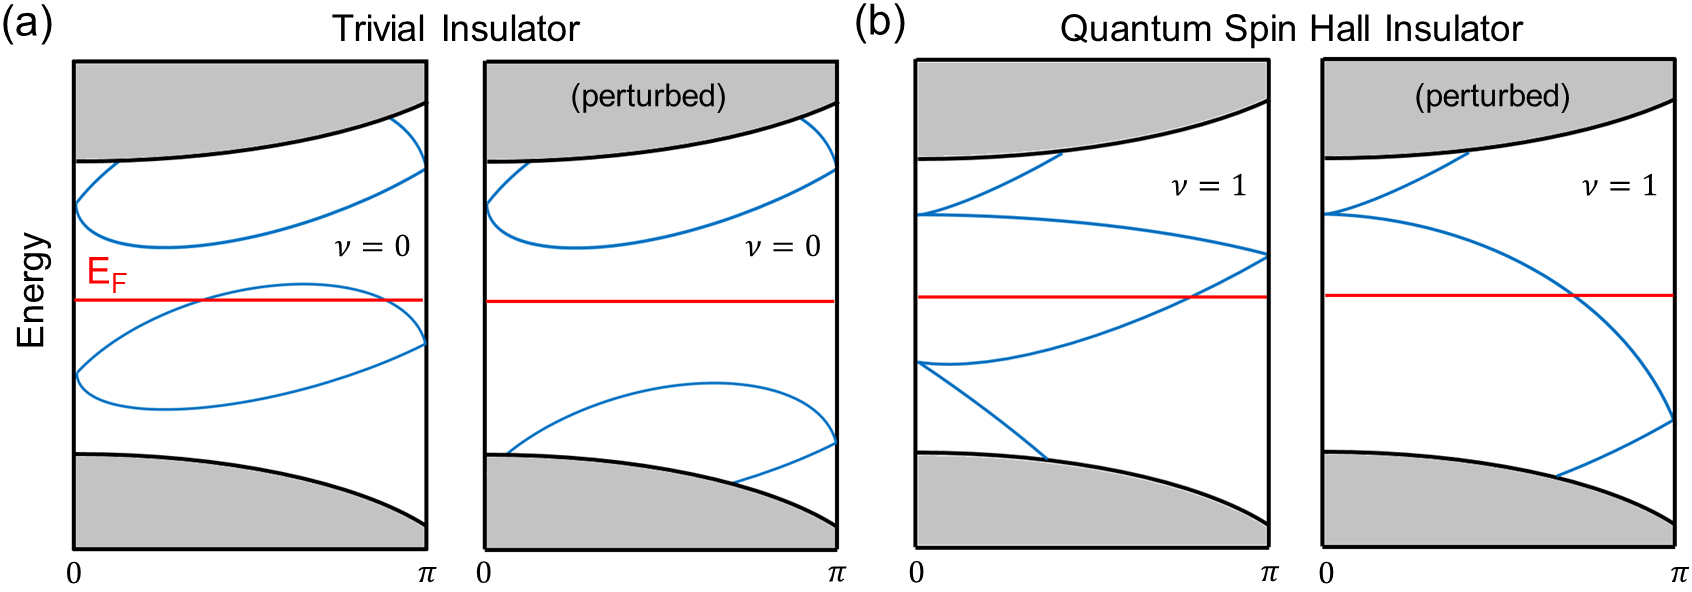
\includegraphics[width=1.0\textwidth]{Z2_perturbed.png}
        \caption[Schematic plots of two topologically different band structures]{Schematic band structure of 1D ribbon cutting from a 2D (a) trivial insulator ($\nu$ = 0) and (b) quantum spin Hall insulator ($\nu$ = 1), where the blue lines indicate the edge states.}
        \label{fig:Z2}
    \end{figure}
    
There are several approaches to calculate the $Z_2$ invariant. The most intuitive way is to exploit bulk-boundary correspondence by calculating the edge states dispersion. This method can be directly implemented by means of standard density functional theory (DFT) calculations. Here is an easy example to understand $Z_2$ invariants by the bulk property. If a system with conserved $S_z$, up and down spins have their individule Chern numbers $n_{\uparrow}$ and $n_{\downarrow}$. Due to TR-symmetry, $n_{\uparrow} + n_{\downarrow} = 0$. The spin Hall conductivity is defined by $n_{\sigma}$ = $(n_{\uparrow} - n_{\downarrow})/2$, and the $Z_2$ invariant can be calculated simply by $Z_2 = n_{\sigma}$ mod 2. However, in real systems, $S_z$ is not conserved due to the presence of spin-orbit coupling, so this is not an generic way to calculate $Z_2$ invariants.


One approach proposed by Fu and Kane \cite{fu2006time} is to first define an unitary matrix $w_{ij} (\textbf{k}) = \langle u_i(\textbf{k}) | \Theta | u_j(-\textbf{k}) \rangle$, which has the property, $w^T (\textbf{k}) = -w (-\textbf{k}) $, due to anti-unitary TR-operator $\Theta$. At four TRIM, $\textbf{k}$ and $-\textbf{k} $ are the same, and hence $w(\Lambda_a)$ is anti-symmetric. The $Z_2$ invariant can be calculated through the following formula when $| u_i(\textbf{k}) \rangle$ is chosen to be continuous throughout the BZ:
	\begin{equation}
		\label{Z2_1}
		\begin{aligned}
			(-1)^{\nu} = 
			\prod_{a=1}^{4}  \frac{ \text{Pf} (w(\Lambda_a) ) }{ \sqrt{\text{Det}( w(\Lambda_a) )} }.
		\end{aligned}
	\end{equation}
If the crystal structure has inversion symmetry (or centrosymmetry), the Eq. (\ref{Z2_1}) can be simplified by examining the parities for each occupied Kramer pairs at TRIM,
	\begin{equation}
		\label{Z2_2}
		\begin{aligned}
			(-1)^{\nu} = 
			\prod_{a=1}^{4} \prod_{n}^{N_{occ}/2}  \xi_{n}(\Lambda_a),
		\end{aligned}
	\end{equation}
where $\xi(\Lambda_a)$ is the parity of wavefunction at $\Lambda_a$ \cite{fu2007topological}.
Fu and Kane also reported another method \cite{fu2006time} to calculate $Z_2$ invariant by inspecting the Berry connection and curvature in the half Brillouin zone (BZ):
	\begin{equation}
		\begin{aligned}
			\nu = \frac{1}{2 \pi} \left[ \oint_{\partial B} \textbf{A} \cdot d\textbf{l} - \int_B \Omega d^2k \right] \hspace{20pt}  \text{mod. 2}
		\end{aligned}
	\end{equation}
with the constraint that the gauge used to obtain the Berry connection
{\bf A} must respect TR symmetry. For non-trivial case, this is known as the obstruction to the Stokes theorem. In other words, if there exists a smooth gauge in the half BZ, then the Stokes theorem holds, and the system is topologically trivial. This method is also applied by Fukui and Hatsugai in their discretized method to check the number of nontrivial plaquettes \cite{fukui2007quantum}.

%{\bf Wannier charge center}

Now, we discuss the situation in three dimension. In quantum anomalous Hall (QAH) effect, the 3D version is associated with stacked 2D QAH layers, and we can use three Chern numbers ($C_1$, $C_2$, $C_3$) to characterize such systems, where $C_1$, $C_2$, and $C_3$ are corresponding to ($k_2$, $k_3$), ($k_1$, $k_3$), and ($k_1$, $k_2$) planes, respectively. The Hall conductivity in 3D QAH insulators is no longer quantized and is proportional to the density of stacked 2D layers. For example, for a (0, 0, $C_3$) QAH insulator with a lattice ${\bf a}_1$, ${\bf a}_2$, and ${\bf a}_3$, the Hall conductivity is $\sigma_{xy} = C_3 (e^2/2\pi \hbar) (1/|{\bf a}_3|)$ \cite{vanderbilt2018berry}. 

For QSH effect in 3D, the situation is different from QAH effect, and it was studied independently Fu, Kane and Mele \cite{fu2007}, as well as Morre and Balents \cite{moore2007topological}, as well as Roy \cite{roy2009topological}. Moore and Balents gave the non-trivail ones a name, ``topological insulator'' (TI), and they can be further divided into strong TI insulator and weak TI. In particular, the strong TI has special surface states that distingushed from 3D QAH systems. The QSH effect in 2D, a single $Z_2$ invariant is used to identify the band topology of a single plane BZ associated with four TRIM. In 3D, we have eight TRIM, and thus there are many choices to get a plane associated with four TRIM. Each plane is an individual 2D QSH system related to a $Z_2$ value, and it seems we can choose six planes, and thus six $Z_2$ invariants to describe a 3D. It turns out, these $Z_2$ values are not independent with each other. As a matter of fact, it takes only four $Z_2$ values to fully characterize a 3D QSH system. The $Z_2$ topological indices are mostly written by ($\nu_0$;$\nu_1\nu_2\nu_3$), where $\nu_0$ is the strong index, and the other three are the weak indices. Similar to Eq. (\ref{Z2_1}) and (\ref{Z2_2}), the topological indices can be calculated through
	\begin{equation}
		\label{Z2_1}
		\begin{aligned}
			&(-1)^{\nu_0} = 
			\prod_{a=1}^{8}  \delta_a,\\
			&(-1)^{\nu_{i=1,2,3}} = 
			\prod_{a=1}^{4}  \delta_a.
		\end{aligned}
	\end{equation}
where $\delta_a = \text{Pf} (w(\Lambda_a) )/ \sqrt{\text{Det}( w(\Lambda_a))  }$. As described above, the strong index involves all eight TRIM while weak indices only associate with four TRIM on plane $k_{i=1,2,3} = \pi$. In a 3D TR-invariant system, an insulator with $\nu_0=1$ is called a strong TI. For those with $\nu_0=0$, one of the $\nu_{i=1,2,3}=1$ is called a weak TI. The one with all four topological indices being 0 is a trivial insulator.

The $Z_2$ indices characterize the number of intersections between surface states and Fermi level being odd or even. If the number of intersection is odd, the surface states are protected by the TR-symmetry. In a strong TI, the surface Fermi arc encloses an odd number of Dirac points, and this ensures a topologically protected surface Dirac cone on any surface of the system. Besides, the surface states on Dirac cone has a distinct property known as spin-momentum locking -- the spin degree of freedom is locked to its momentum. We call it ``strong'' because these surface properties are robust against small perturbation like small disorder as long as TR-symmetry is present.

On the other hand, the weak TI phase can be regarded as stacked 2D QSH layers along $\textbf{G} = \nu_1 \textbf{b}_1 + \nu_2 \textbf{b}_2 + \nu_3 \textbf{b}_3$ “module 2” reciprocal lattice vector. 
On the side surfaces of a stacked QSH layers, the 2D topological surface states are formed due to the collection of 1D edge states by each QSH layer. However, the top and bottom surfaces are simply trivial surfaces. The term ``weak'' here is related to the translational symmetry along $\textbf{G}$, and we say that surface states in weak TI are not robust against perturbations that break translational symmetry (like dislocation). However, this sensitivity renders us some interesting phenomena, such as anisotropic edge modes, quantized charge polarization, and bound states at dislocation defects.

The topological edge/surface states in QSH effect have great potential to facilitate the advance in science and technology. The followings are some of the possibilities. In magnetic topological insulator or QAH insulator, the backs-cattering-immune property is promissing for dissipaionless topologcical electronics. The spin-momentum-locked properties in topological insulators can be used for spintronic devices. The junction of a topological insulator and an s-wave superconductor is promising for the realization of Majorana particles, and this can help the realization of fault-tolerant quantum computing. As a result, it is important to know how to manipulate the topological surface states by controlling the transitions between topological phases.




	
    \pagebreak
    
	
    %\subsection*{Overview of Remaining Chapters}
    \addcontentsline{toc}{subsection}{Overview of Remaining Chapters}
	{\centering
		\vspace{12pt} Overview of Remaining Chapters
	    \par
	}
    In the following, we describe the methods employed in this dissertation including density functional theory, evolutionary algorithm and machine learning. The results contain our studies related to computational search for new ternary superhard materials and topological phase transitions in quantum materials. In our B-C-N study, we exploited existing online database to build machine learning models for predicting mechanical properties for the B-C-N system. Guided by machine learning prediction, we then used evolutionary algorithm to search for superhard B-C-N compounds. For the B-N-O study, we adopted a recursive, self-improving method based on the data generated by evolutionary algorithm to find ternary B-N-O compounds with high cohesive energy and high hardness.
    
    For the topological phase transition research, we have studied the transition in ZrTe$_5$ between strong TI phase to weak TI phase driven by uniaxial strain. Besides, we have also studied the transition between strong TI phase and trivial phase in lanthanum monopnictides. In particular, we found LaN has a low-temperature, ferroelectric structure, which enriches both its structural and topological phase transitions. 
    


    \clearpage

    %\chapter{2 METHODS}
    \addtocounter{numch}{1}
	\addcontentsline{toc}{chapter}{\hspace{4pt}  \the\value{numch} \hspace{4pt} METHODS}
	{\centering
		\vspace{0pt} \hspace{0pt} \par
	}
	{\centering
		\vspace{56pt} CHAPTER  \the\value{numch}
	}
	{\centering\singlespacing
		METHODS
	    \par
	}
	{\centering
		\vspace{0pt} \hspace{0pt} \par
	}

    %\subsection*{Density Functional Theory}
    \addcontentsline{toc}{subsection}{Density Functional Theory}
	{\centering
		\vspace{12pt} Density Functional Theory
	    \par
	}

One of the primary goals in solid state physics and quantum chemistry is to determine the electronic structure because it arguably determines all of the physical properties of a material. In principle, the electronic structure of a system can be obtained by solving the many-body Shr\"{o}dinger equation. However, only small systems that containing very small number of electrons like helium atom, hydrogen molecule, and lithium atom can be accurately solved using the variational method. The main difficulty in solving electronic structure of many-electron systems lies in the lack of proper treatment of electron-electron interactions. Therefore, solving the electronic structure in an accurate and efficient way is still challenging today.

The Hartree-Fock (HF) theory is the first wavefunction-based approach that captures the fundamental ingredients to solve the many-body  Shr\"{o}dinger equation using a mean-field approximation for electron-electron interaction and also using the Slater determinant to be the approximate many-body wavefunction \cite{hartree1928wave,fock1930naherungsmethode,slater1951simplification}. However, the electron-electron interaction in the HF method is not precise enough for it to obtain accurate many-body wavefunction. Despite of the inaccuracy, the HF theory laid a good foundation for its successors known as post-HF approaches including M\o ller–Plesset perturbation theory, Coupled cluster, configuration interaction, etc. The post-HF methods show higher accuracy, and are widely used in modern quantum chemistry calculations. However, such calculations require huge computational time.

Different from methods focusing on solving many-body wavefunction, another category -- density-based method, aims at solving electron density distribution to obtain a system's physical properties. The pioneer of density-based method is the Thomas-Fermi (TF) model , which was independently proposed by Thomas and Fermi \cite{thomas1927calculation,fermi1928statistische}. The ideas of using electron density (instead of wavefunction) as the central variable and local density approximation (LDA) to compute the total energy. 
The LDA basically says that the properties of an inhomogeneous electron gas is locally identical to those of homogeneous one. According to the TF model, the total kinetic energy of the electrons can be expressed in terms of electron density distribution  $\rho(\textbf{r})$ without any wavefunction information. In the TF model, the total energy functional is
	\begin{equation}
		\label{eq:tf}
		\begin{aligned}
			E_{TF}[\rho(\textbf{r})] = T_{TF}[\rho(\textbf{r})] + \int \rho(\textbf{r})v_{ext}(\textbf{r})d\textbf{r} +
			\frac{1}{2} \int \int \frac{\rho(\textbf{r}) \rho(\textbf{r}')}{\left|\textbf{r} - \textbf{r}'  \right|}d\textbf{r} d\textbf{r}',
		\end{aligned}
	\end{equation}
where $\rho$ is electron density, $v_{ext}$ is external potential
	\begin{equation}
		\begin{aligned}
			v_{ext} = -\sum_i \int \frac{Z_i}{\left| \textbf{r}-\textbf{R}_i \right|} d\textbf{r},
		\end{aligned}
	\end{equation}
and $T_{TF}$ is kinetic energy functional, which can be expressed as
	\begin{equation}
		\begin{aligned}
			%T[\rho(\textbf{r})] \approx
			T_{TF}[\rho(\textbf{r})] = t_0\int \rho^{5/3}(\textbf{r}) d\textbf{r},
		\end{aligned}
	\end{equation}
where $t_0$ is a coefficient, $\frac{3}{10}(3\pi^2)^{2/3}$ in atomic unit. The last term in Eq. (\ref{eq:tf}) is the classical eletrostatic energy between electrons, which is also known as Hartree energy. In quantum mechanics, one needs to compute the expected value of kinetic energy through the many-body wavefunction, which has 3$N$ variables and difficult to solve. Here, the TF model demonstrates that density-based approaches can dramatically reduce the number of variables from 3$N$ to 3. However, the TF model is just regarded as a toy model due to imprecise expression for kinetic energy and omission of quantum mechanical electron-electron interactions. In 1928, Dirac added an exchange-energy functional term to refine the TF model \cite{dirac1930note}, but it did not eliminate the primary errors from crude kinetic energy and electron correlation energy. Hence, density-based methods were not considered to be practical for real materials. Solving a quantum-mechanical many-body problem using only three spacial variables was regarded to be impossible for more than 35 years. Until 1964, the theoretically exact density functional theory was proposed by Hohenberg and Kohn, and today it has become the most polpular method to study many-electron systems like solids and molecules.

Density functional theory (DFT) is a quantum-mechanical theory that can be derived from the many-body Schr\"{o}dinger equation. In the following, we introduce the formalism of DFT from many-body Hamiltonian, Born-Oppenheimer approximation, Hohenberg-Kohn theorems, self-consistent Kohn-Sham equation, and exchange-correlation energy functional used in this dissertation. Besides, we also introduce practical implementation of pseudopotential techniques that largely reduce the computation time.

In a system composed of electrons and nuclei, the behavior of such a system is govorned by its total many-body Hamiltonian $\hat{\mathcal{H}}$. It includes nuclear part $\hat{\mathcal{H}}_n$ and electronic part $\hat{\mathcal{H}}_e$. Here, we put the nucleus-electron interaction in $\hat{\mathcal{H}}_{e}$. Their mathematical forms in atomic units ($\hbar$=1, $m_e$=1, $e$=1) are shown as follows.
	\begin{equation}
	\begin{aligned}
        &\hat{\mathcal{H}} = \hat{\mathcal{H}}_{n} + \hat{\mathcal{H}}_{e} \\
        &\hat{\mathcal{H}}_{n} = -\frac{1}{2}\sum_N \frac{1}{M_N}\nabla^2 + \sum_{N<M} \frac{Z_NZ_M}{\left| \textbf{R}_N-\textbf{R}_M \right|}\\
        &\hat{\mathcal{H}}_{e} = -\frac{1}{2}\sum_i \nabla_i^2 + \sum_{i<j} \frac{1}{\left| \textbf{r}_i-\textbf{r}_j \right|} -\sum_{Ni} \frac{Z_N}{\left| \textbf{R}_N-\textbf{r}_i \right|} \\
	\end{aligned}
	\end{equation}
One can obtain all of the information of the system by solving the time-independent Schr\"{o}dinger equation
	\begin{equation}
	\begin{aligned}
        & \hat{\mathcal{H}}\Theta(\{\textbf{R}\},\{\textbf{r}\}) = E_{tot}\Theta(\{\textbf{R}\},\{\textbf{r}\}).
	\end{aligned}
	\end{equation}
However, this is the primary difficulty in electronic structure problem and unsolvable for many-electron systems. The next step to approach the solution is Born-Oppenheimer (BO) approximation, where it assumes the wavefunctions of nuclei and electrons in a system can be separated because the motions of nuclei are much faster than that of electrons based on their mass difference ($M_n \gg m_e$). The mathematical form of BO approximation is expressed as
	\begin{equation}
	\begin{aligned}
        \Theta(\{\textbf{R}\},\{\textbf{r}\}) = \Phi(\{\textbf{R}\})\Psi(\{\textbf{r}\}),
    \end{aligned}
	\end{equation},
where $\Phi(\{\textbf{R}\})$ is the nuclear wavefunction, and $\psi(\{\textbf{r}\})$ is the electronic wavefunction. Next, one can solve the electronic Schr\"{o}dinger by treating the nucleus positions as parameters, and the nuclei-electron interaction becomes the external potential felt by electrons:
	\begin{equation}
	\begin{aligned}
        \hat{\mathcal{H}}_e \Psi(\{\textbf{r}\})=E_e \Psi(\{\textbf{r}\}).
    \end{aligned}
	\end{equation}
In fact, this is the starting point of most of the electronic structure theories. Once the E$_e$ is solved, one can then calculate the total energy E$_{tot}$ of a system by treating nuclei as point charges, $i.e.$ in a classical way. In other words, at 0 K, one can neglect the kinetic energy of nuclei, and the total energy $E_{tot}$ is the sum of electronic energy and the electrostatic energy between nuclei:
	\begin{equation}
	\begin{aligned}
	    & E_{tot} = E_e + E_{NN}, \\
        & E_{NN} = \sum_{N<M} \frac{Z_NZ_M}{\left| \textbf{R}_N-\textbf{R}_M \right|}.
    \end{aligned}
	\end{equation}

We next discuss the foundation of the DFT, Hohenberg-Kohn theorems and Kohn-Sham equation. In the seminal paper by Hohenberg and Kohn \cite{DFT_1}, they prove that in an non-degenerate electronic system subjected to an external potential $v_{ext}$(\textbf{r}), such $v_{ext}$(\textbf{r}) has an one-to-one relationship with electron density. Or more precisely: \newline

	{Theorem 1:
	  \textit{The external potential, and hence the Hamiltonian is uniquely  \\ 
	  \vspace{0pt}  \hspace{74pt} determined by a single and specific electron density.}
	  \singlespacing
	 }
Based on Theorem 1, in principle, $all$ of the properties, or expectation values of $all$ observables, of an electronic system can be determined as long as the ground state electron density is given. The second Hohenberg-Kohn theorem follows the idea of the TF model that the total energy of electronic system can be expressed as a density functional:
	\begin{equation}
		\label{eq:hk}
		\begin{aligned}
			E[\rho(\textbf{r})] &= T[\rho(\textbf{r})] + V_{ee}[\rho(\textbf{r})] +V_{eN}[\rho(\textbf{r})] \\
			& = F[\rho(\textbf{r})] +V_{eN}[\rho(\textbf{r})],
		\end{aligned}
	\end{equation}
where $F[\rho(\textbf{r})]$ does not depend on the external potential $V_{ext}$(\textbf{r}), and is known as universal functional. Hohenber and Kohn shows that minimum of energy functional can be obtained through variational principle, and the second theorem is abtained:\newline

	 {Theorem 2:
	  \textit{The electron density that minimizes the total energy functional is the   \\ 
	  \vspace{0pt}  \hspace{74pt} unique ground state density.  }
	  \singlespacing
	 }
	 
Although the powerful Hohenberg-Kohn theorems lay a solid foundation for DFT, they do not provide a practical framework like the mathematical forms of $T[\rho(\textbf{r})]$ and $V_{ee}[\rho(\textbf{r})]$ to obtain the ground sate density. One year later, Kohn and Sham proposed the Kohn-Sham equation, which provides a practical scheme to solve ground state density as well as ground state total energy \cite{DFT_2}. The key ingredient makes the success of Kohn-Sham equation is that there exist a local single-particle potential, which is able to reproduce the ground state density of the real interacting system. To derive the Kohn-Sham equation, we start from Eq. (\ref{eq:hk}), and our task is to minimize the total energy $E$[$\rho$(\textbf{r})] for a system with a specific external potential $v_{ext}$ and fixed number of electrons $N$. 
	\begin{equation}
	\label{variation}
	\begin{aligned}
        0 = \delta \left\{E[\rho] - \mu\int \rho(\textbf{r}) d\textbf{r} \right\} = \int d\textbf{r} \left[ \frac{\delta F[\rho]}{\delta \rho(\textbf{r})} + v_{ext}(\textbf{r}) - \mu \right] \delta \rho(\textbf{r}),
    \end{aligned}
	\end{equation}
where $\mu$ is the Lagrange multiplier. The obtained Euler equation is
	\begin{equation}
	\label{euler1}
	\begin{aligned}
        \frac{\delta F[\rho]}{\delta \rho(\textbf{r})} + v_{ext}(\textbf{r}) = \mu.
    \end{aligned}
	\end{equation}
The next step is the essence of Kohn-Sham equation: creating a non-interacting system with a different external potential $v_{KS}$(\textbf{r}), and such a new potential contains the original $v_{ext}$(\textbf{r}) and all of the electron-electron interactions. Therefore, we can divide the interacting kinetic energy into the non-interacting part and the interacting part,
	\begin{equation}
	\begin{aligned}
        T[\rho] = T_s[\rho] + T_c[\rho],
    \end{aligned}
	\end{equation}
where $T_s[\rho]$ is the non-interacting kinetic energy (denoting s for single-particle), and $T_c[\rho]$ is the correlation part in kinetic energy (denoting c for correlation). The $V_{ee}$ can also be represented by
	\begin{equation}
	\begin{aligned}
        V_{ee}[\rho] = V_H[\rho] + E_{x}[\rho] + V_{c}[\rho],
    \end{aligned}
	\end{equation}
where $V_H[\rho]$ is the classic Hartree energy, $E_{x}[\rho]$ is the quantum-mechanical exchange energy, and $V_{c}[\rho]$ is the correlation part of electron-electron interaction. The correlation energy is then $E_{c}[\rho] = T_{c}[\rho] + V_{c}[\rho]$. In DFT, the exchange energy and correlation energy functionals are further combined as exchange-correlation energy functional
	\begin{equation}
	\label{Exc}
	\begin{aligned}
        E_{xc}[\rho] &= E_{x}[\rho] + E_{c}[\rho]
    \end{aligned}
	\end{equation}
Therefore, the total energy functional can be represented as
	\begin{equation}
	\begin{aligned}
        E[\rho] &= T[\rho] + V_{ee}[\rho] + V_{eN}[\rho] \\  &= T_s[\rho] + V_H[\rho] + E_{xc}[\rho] +            V_{eN}[\rho].
    \end{aligned}
	\end{equation}
The new universal functional becomes
	\begin{equation}
	\begin{aligned}
        F[\rho] = T_s[\rho] + V_H[\rho] + E_{xc}[\rho].
    \end{aligned}
	\end{equation}
From Eq. (\ref{variation}) and (\ref{euler1}), the new Euler equation hence becomes
	\begin{equation}
	\label{euler2}
	\begin{aligned}
        \mu &= \frac {T_s[\rho]}{\delta \rho(\textbf{r})} + \frac {V_H[\rho]}{\delta \rho(\textbf{r})} +
       \frac {E_{xc}[\rho]}{\delta \rho(\textbf{r})} + v_{ext}(\textbf{r}) \\ &= \frac {T_s[\rho]}{\delta \rho(\textbf{r})} + v_H(\textbf{r}) + v_{xc}(\textbf{r}) + v_{ext}(\textbf{r}) \\
       &= \frac {T_s[\rho]}{\delta \rho(\textbf{r})} + v_{KS}(\textbf{r}),
    \end{aligned}
	\end{equation}
where $v_{H}(\textbf{r})$ is Hartree potential, $v_{xc}(\textbf{r})$ is exchange-correlation potential, and we also introduce Khon-Sham potential $v_{KS}(\textbf{r}) = v_{H}(\textbf{r})+ v_{xc}(\textbf{r}) + v_{ext}(\textbf{r})$. Comparing Eq. (\ref{euler2}) and (\ref{euler1}), we find that 
by simply rearrange the energy functional terms, we can obtain the ground state density of an interacting system by solving the alternative non-interacting system subjected to Kohn-Sham potential $v_{KS}(\textbf{r})$.

Now, to deal with the non-interacting system, we can obtain the ground state density by solving the $N$ single-electron Kohn-Sham equations.
	\begin{equation}
	\label{ks_eq}
	\begin{aligned}
        \left[ -\frac{1}{2}\nabla^2 + v_{KS}(\textbf{r})  \right] \psi_i(\textbf{r}) = \epsilon_i \psi_i(\textbf{r})
    \end{aligned}
	\end{equation}
The electron density corresponds to a set of Khon-Sham orbitals {$\psi_i$} is
	\begin{equation}
	\label{density}
	\begin{aligned}
        \rho_0(\textbf{r}) = \sum_{i}^{occ} \left| \psi_i(\textbf{r}) \right|^2.
    \end{aligned}
	\end{equation}
The obtained density is not the solution yet. The reason is that the Kohn-Sham potential $v_{KS}(\textbf{r})$ depends on the density $\rho(\textbf{r})$, and $v_{KS}(\textbf{r})$ also depends on $\psi_i(\textbf{r})$. Hence, we need to solve Eq. (\ref{ks_eq}) and (\ref{density}) in a self-consistent way like in the HF method. Once solved, the ground state energy can be calculated by
	\begin{equation}
	\label{tot_energy}
	\begin{aligned}
        E_0 = \sum_{i}^N \epsilon_i - \frac{1}{2} \int \int d\textbf{r}d\textbf{r}' \frac{\rho_0(\textbf{r}) \rho_0(\textbf{r})'} {\left|\textbf{r} - \textbf{r}' \right|} + E_{xc}[\rho_0] - \int d\textbf{r} \rho_0(\textbf{r}) v_{xc}(\textbf{r})
    \end{aligned}
	\end{equation}
The expression of for total energy in Eq. (\ref{tot_energy}) is in principal exact, but in practice, the $E_{xc}[\rho]$ and $v_{xc}(\textbf{r})$ are unknown, and needed to be approximated.

In our previous discussion for the TF model, the concept of LDA has been considered for the kinetic energy functional. Here, in the context of exchange-correlation energy functional, we first introduce the famous LDA, which has brings tremendous success for DFT in the studies of solids and molecules in the real world. The LDA assumes that the exchange-correlation energy functional is the sum of the pieces of exchange-correlation energies within the infinitesimal volumes, where the exchange-correlation energy is based on the result of homogeneous electron gas (HEG): 
	\begin{equation}
	\begin{aligned}
        E_{xc}^{LDA}[\rho] = \int \rho(\textbf{r}) \varepsilon_{xc}^{LDA}(\rho(\textbf{r})) d\textbf{r},
    \end{aligned}
	\end{equation}
and hence the exchange-correlation potential is
	\begin{equation}
	\begin{aligned}
        v_{xc}^{LDA}(\textbf{r}) = \frac{\delta E^{LDA}}{\delta \rho(\textbf{r})} = \varepsilon_{xc}^{LDA}(\rho(\textbf{r})) + \rho(\textbf{r})\frac{\partial \varepsilon_{xc}^{LDA}(\rho)}{\partial \rho(\textbf{r})},
    \end{aligned}
	\end{equation}
where $\varepsilon_{xc}^{LDA}$ can be divided into exchange part and correlation part,
	\begin{equation}
	\begin{aligned}
        \varepsilon_{xc}^{LDA} = \varepsilon_{x}^{HEG} +\varepsilon_{c}^{HEG}.
    \end{aligned}
	\end{equation}
The exchange energy functional in the LDA is
	\begin{equation}
	\begin{aligned}
        E_{x}^{LDA}[\rho] = \int \rho(\textbf{r}) \varepsilon_{x}^{HEG}(\rho(\textbf{r})) d\textbf{r},
    \end{aligned}
	\end{equation}
The exchange part was carried out by Dirac with an exact form \cite{dirac1930note},
	\begin{equation}
	\begin{aligned}
        \varepsilon_{x}^{HEG} = -\frac{3}{4} \left( \frac{3}{\pi}\right)^{\frac{1}{3}} \rho^{\frac{1}{3}} .
    \end{aligned}
	\end{equation}
The correlation part does not have an exact form, and its mathematical form is mostly parametrised by the results of using quantum Monte Carlo method to solve HEG systems. There are many examples including Perdew-Zunger \cite{perdew1981self}, Perdew-Wang \cite{perdew1992accurate}, Vosko-Wilk-Nusair \cite{vosko1980accurate}, etc. As an example for many different forms, the Perdew-Zunger's LDA formula \cite{perdew1981self} is expressed as
	\begin{equation}
	\begin{aligned}
        \varepsilon_c^{PZ} (r_s)= 
        \begin{cases}
            A \text{ ln } r_s + B + Cr_s \text{ ln } r_s + Dr_s \hspace{20pt} r_s \le 1 \\
          \gamma/(1+\beta_1\sqrt{r_s}+\beta_2r_s) \hspace{67pt} r_s > 1,
    \end{cases}   
    \end{aligned}
	\end{equation}
where $r_s$ is the Wigner-Seitz radius ($\frac{4}{3}\pi r_s^3 = \frac{1}{\rho}$). $A$, $B$, $C$, and $D$ are parameters based on the results of random phase approximation, while $\gamma$, $\beta_1$, $\beta_2$ are constants based on the precise Quantum Monte Carlo simulation data by Ceperley and Alder \cite{ceperley1980ground}.

For spin-polarized systems, the LDA of exchange-correlation energy functional is called local spin density approximation (LSDA), which depends on two spin densities:
	\begin{equation}
	\begin{aligned}
        E_{xc}^{LSDA}[\rho_{\uparrow}, \rho_{\downarrow}] = \int \rho(\textbf{r}) \varepsilon_{xc}^{HEG}(\rho_{\uparrow}, \rho_{\downarrow}) d\textbf{r},
    \end{aligned}
	\end{equation}
where $\rho = \rho_{\uparrow}+\rho_{\downarrow}$. The exchange part is simply
	\begin{equation}
	\begin{aligned}
        E_{x}^{LSDA}[\rho_{\uparrow}, \rho_{\downarrow}] = \frac{1}{2} (E_{x}^{LDA}[2\rho_{\uparrow}]  + E_{x}^{LDA}[2\rho_{\downarrow}] ).
    \end{aligned}
	\end{equation}
The spin correlation energy density is constructed by interpolating the extreme values. It has a form of $\varepsilon_c = \varepsilon_c(\rho, \zeta)$, where $\zeta = (\rho_{\uparrow}-\rho_{\downarrow})/\rho $ is the relative spin-polarization. 

Since in the real systems, the density $\rho$({\bf r}) is spacially varying, adding higher order terms like $\nabla \rho({\bf r})$ and $\nabla^2 \rho({\bf r})$ should better describe the exchange-correlation energy functional. The first implementation of this idea is gradient expansion approximation (GEA), which systematically increases higher order gradient terms. However, it was found that the GEA with first order correction hardly improves the results comparing with LDA \cite{perdew1996generalized}. Since adding the first order correction fails to improve the functional, including higher order terms cannot be justified. People latter found that the functional could be improved by more general functions with only $\rho(\textbf{r})$ and $\nabla \rho(\textbf{r})$ as variables. Such functional is known as generalized gradient approximation (GGA), and they have a form as
	\begin{equation}
	\begin{aligned}
        E_{xc}^{GGA}[\rho_{\uparrow}, \rho_{\downarrow}] = \int d\textbf{r} f(\rho_{\uparrow},\rho_{\downarrow}, \nabla \rho_{\uparrow}, \nabla \rho_{\downarrow})
    \end{aligned}
	\end{equation}
Again, like in LDA, the exchange and correlation functionals are separated, $E_{xc}^{GGA} = E_{x}^{GGA} + E_{c}^{GGA}$. The GGA exchange functional has a form like LSDA
	\begin{equation}
	\begin{aligned}
        &E_{x}^{GGA}[\rho_{\uparrow}, \rho_{\downarrow}] = \frac{1}{2} (E_{x}^{GGA}[2\rho_{\uparrow}]  + E_{x}^{GGA}[2\rho_{\downarrow}] ) \\
        &E_x^{GGA}[\rho] = \int \rho(\textbf{r}) \varepsilon_{x}^{HEG}(\rho) F_x(s) d\textbf{r}
    \end{aligned}
	\end{equation}
where $F_x(s)$ is a function that modifies the LDA exchange functional with $s$ being a function of $\rho$ and $|\nabla \rho|$ \cite{perdew1996generalized}.
The correlation part of GGA does not have an unified form. One of the expressions introduced by Perdew, Burke, and Ernzerhof (PBE) has the following form \cite{perdew1996generalized}:
	\begin{equation}
	\begin{aligned}
        E_c^{GGA}[\rho_{\uparrow},\rho_{\downarrow}] = \int \rho(\textbf{r})  \left[ \varepsilon_{c}^{HEG} (\rho, \zeta) + H^{PBE} (\rho, \zeta, t) \right],
    \end{aligned}
	\end{equation}
where $t$ is a function of $\rho$, $\zeta$, and $|\nabla \rho|$.

The performance of DFT results relies on the quality of the approximation for the exchange-correlation energy functional. In general, DFT results based on GGA functional show high accuracy in properties like energies and bond lengths in molecule, as well as lattice constants in solids. However, the LDA and GGA are known to underestimate the energy gap obtained in band structure calculations, which is the so-called ``bandgap problem''. It is known that bandgap estimations based on hybrid functional DFT and GW approximation in many-body perturbation are much more accurate. Since we have used hybrid functional to better estimate the bandgap, we give a brief introduction in the following.

In the hybrid functionals, a portion of non-local exact exchange energy from HF theory is incorporated with the local exchange part in LDA or GGA. The HF exact exchange functional can be calculated by
	\begin{equation}
	\begin{aligned}
        E_x^{HF} = -\frac{1}{2} \sum_{\textbf{k},\textbf{k}'}\sum_{i,j}^{occ} \int \psi_{i{\bf k}}^*({\bf r}) \psi_{j{\bf k}'}^*({\bf r}') \frac{1}{|{\bf r}-{\bf r}'|} \psi_{i{\bf k}}({\bf r'}) \psi_{j{\bf k}'}({\bf r}) d{\bf r} d{\bf r}',
    \end{aligned}
	\end{equation}
where $\psi({\bf r})$ stands for the Khon-Sham orbital. The hybrid functional then has a general form:
	\begin{equation}
	\begin{aligned}
        E_{xc}^{Hybrid} = E_{xc}^{L} + a(E_{xc}^{HF} - E_{x}^{L}),
    \end{aligned}
	\end{equation}
where $E_{xc}^{L}$ is the local exchange-correlation energy functional (like LDA and GGA). A hybrid functional based on PBE local functional is known as PBE0 \cite{perdew1996rationale}, where the value of $a$ is 0.25. Another well-known hybrid functional proposed by Heyd, Scuseria, and Ernzerhof is HSE hybrid functional, where an error function is used to separate
the long-range and the short-range parts \cite{heyd2003hybrid}.
	\begin{equation}
	\begin{aligned}
        \frac{1}{r} = \frac{\text{erfc}(\omega r)}{r} + \frac{\text{erf}(\omega r)}{r}.
    \end{aligned}
	\end{equation}
In the first term, $\text{erfc} (\omega r) = 1 - \text{erf}(\omega r)$. The first and the second terms are the short-range and long-range parts, respectively. $\omega$ is the  is an adjustable parameter. The complete form of HSE hybrid functional is shown as
	\begin{equation}
	\begin{aligned}
        E_{xc}^{HSE} = aE_x^{HF,SR}(\omega) + (1-a)E_x^{PBE,SR}(\omega) + E_x^{PBE,LR}(\omega) + E_c^{PBE}.
    \end{aligned}
	\end{equation}
In HSE06 hybrid functional, used in this dissertation, the values of $a$ and $\omega$ are 0.25 and 0.2, respectively \cite{krukau2006influence}. Basically, GGA functionals (like PBE) can give us reliable results for most properties including total energy, lattice parameters, and strengths of chemical bonds (covalent, ionic, metallic and hydrogen bridge. To study the energy gap between valence and conduction bands, the hybrid functionals can be taken into consideration while it is computationally expensive.

After the discussion of how we can use DFT to calculate the total energy, we next discuss how forces and stresses are computed based on Hellman-Feynman theorem. For a Hamiltonian which can be parametrized by a variable $\lambda$, we have
	\begin{equation}
	\begin{aligned}
        \hat{H}(\lambda) \Psi(\lambda) = E(\lambda). \Psi(\lambda)
    \end{aligned}
	\end{equation}
Based on Hellman-Feynman theorem, the derivative of E with respect to $\lambda$ can be calculated by
	\begin{equation}
	\begin{aligned}
        \frac{\partial E (\lambda)}{\partial \lambda} = \left \langle \Psi (\lambda) \left|  \frac{\partial \hat{H}}{\partial \lambda}   \right|  \Psi (\lambda) \right\rangle.
    \end{aligned}
	\end{equation}
Therefore, the force on the nucleus $I$ is
	\begin{equation}
	\begin{aligned}
        {\bf F}_I({\bf R}) = - \nabla_{\bf R} E({\bf R}) = -\left \langle \Psi ({\bf R})\left|  \nabla_{\bf R} H \right| \Psi({\bf R})   \right \rangle.
    \end{aligned}
	\end{equation}
Stresses can also be calculated using a similar but more complicated expression based on Nielsen {\it et al.} \cite{nielsen1985quantum}.

With the information of forces and stresses, we can do structure relaxation by minimizing both forces and stresses. Here, the procedure of structure relaxation in a DFT code is shown in Fig.  \ref{fig:DFT_flowchart}. At first, we only need to provide the initial crystal structure, and then the code enter the electronic loop to obtain the ground state electron density by solving the Kohn-Sham equation self-consistently, which is also known as the self-consistent field calculation (shown in the yellow box in Fig. \ref{fig:DFT_flowchart}). The update of electron density is done by mixing the new and the old densities, and the convergence criteria include the energy difference (usually less than $10^{-5}$ eV/atom), and also the differences in eigenvalues. Once the self-consistent field is done, the code will calculate the forces and stresses. By means of algorithms like quasi-Newton, and conjugate-gradient methods, the crystal structure can be gradually optimized. The convergence criterion for structure relaxation is usually the force on each atom less than $10^{-2}$ or $10^{-3}$ eV/\AA. The structure relaxation is also important in the procedure of crystal structure prediction, which will be introduced in the next section.

    \begin{figure}[htbp]
        \centering
        \captionsetup{singlelinecheck = false, justification=justified}
        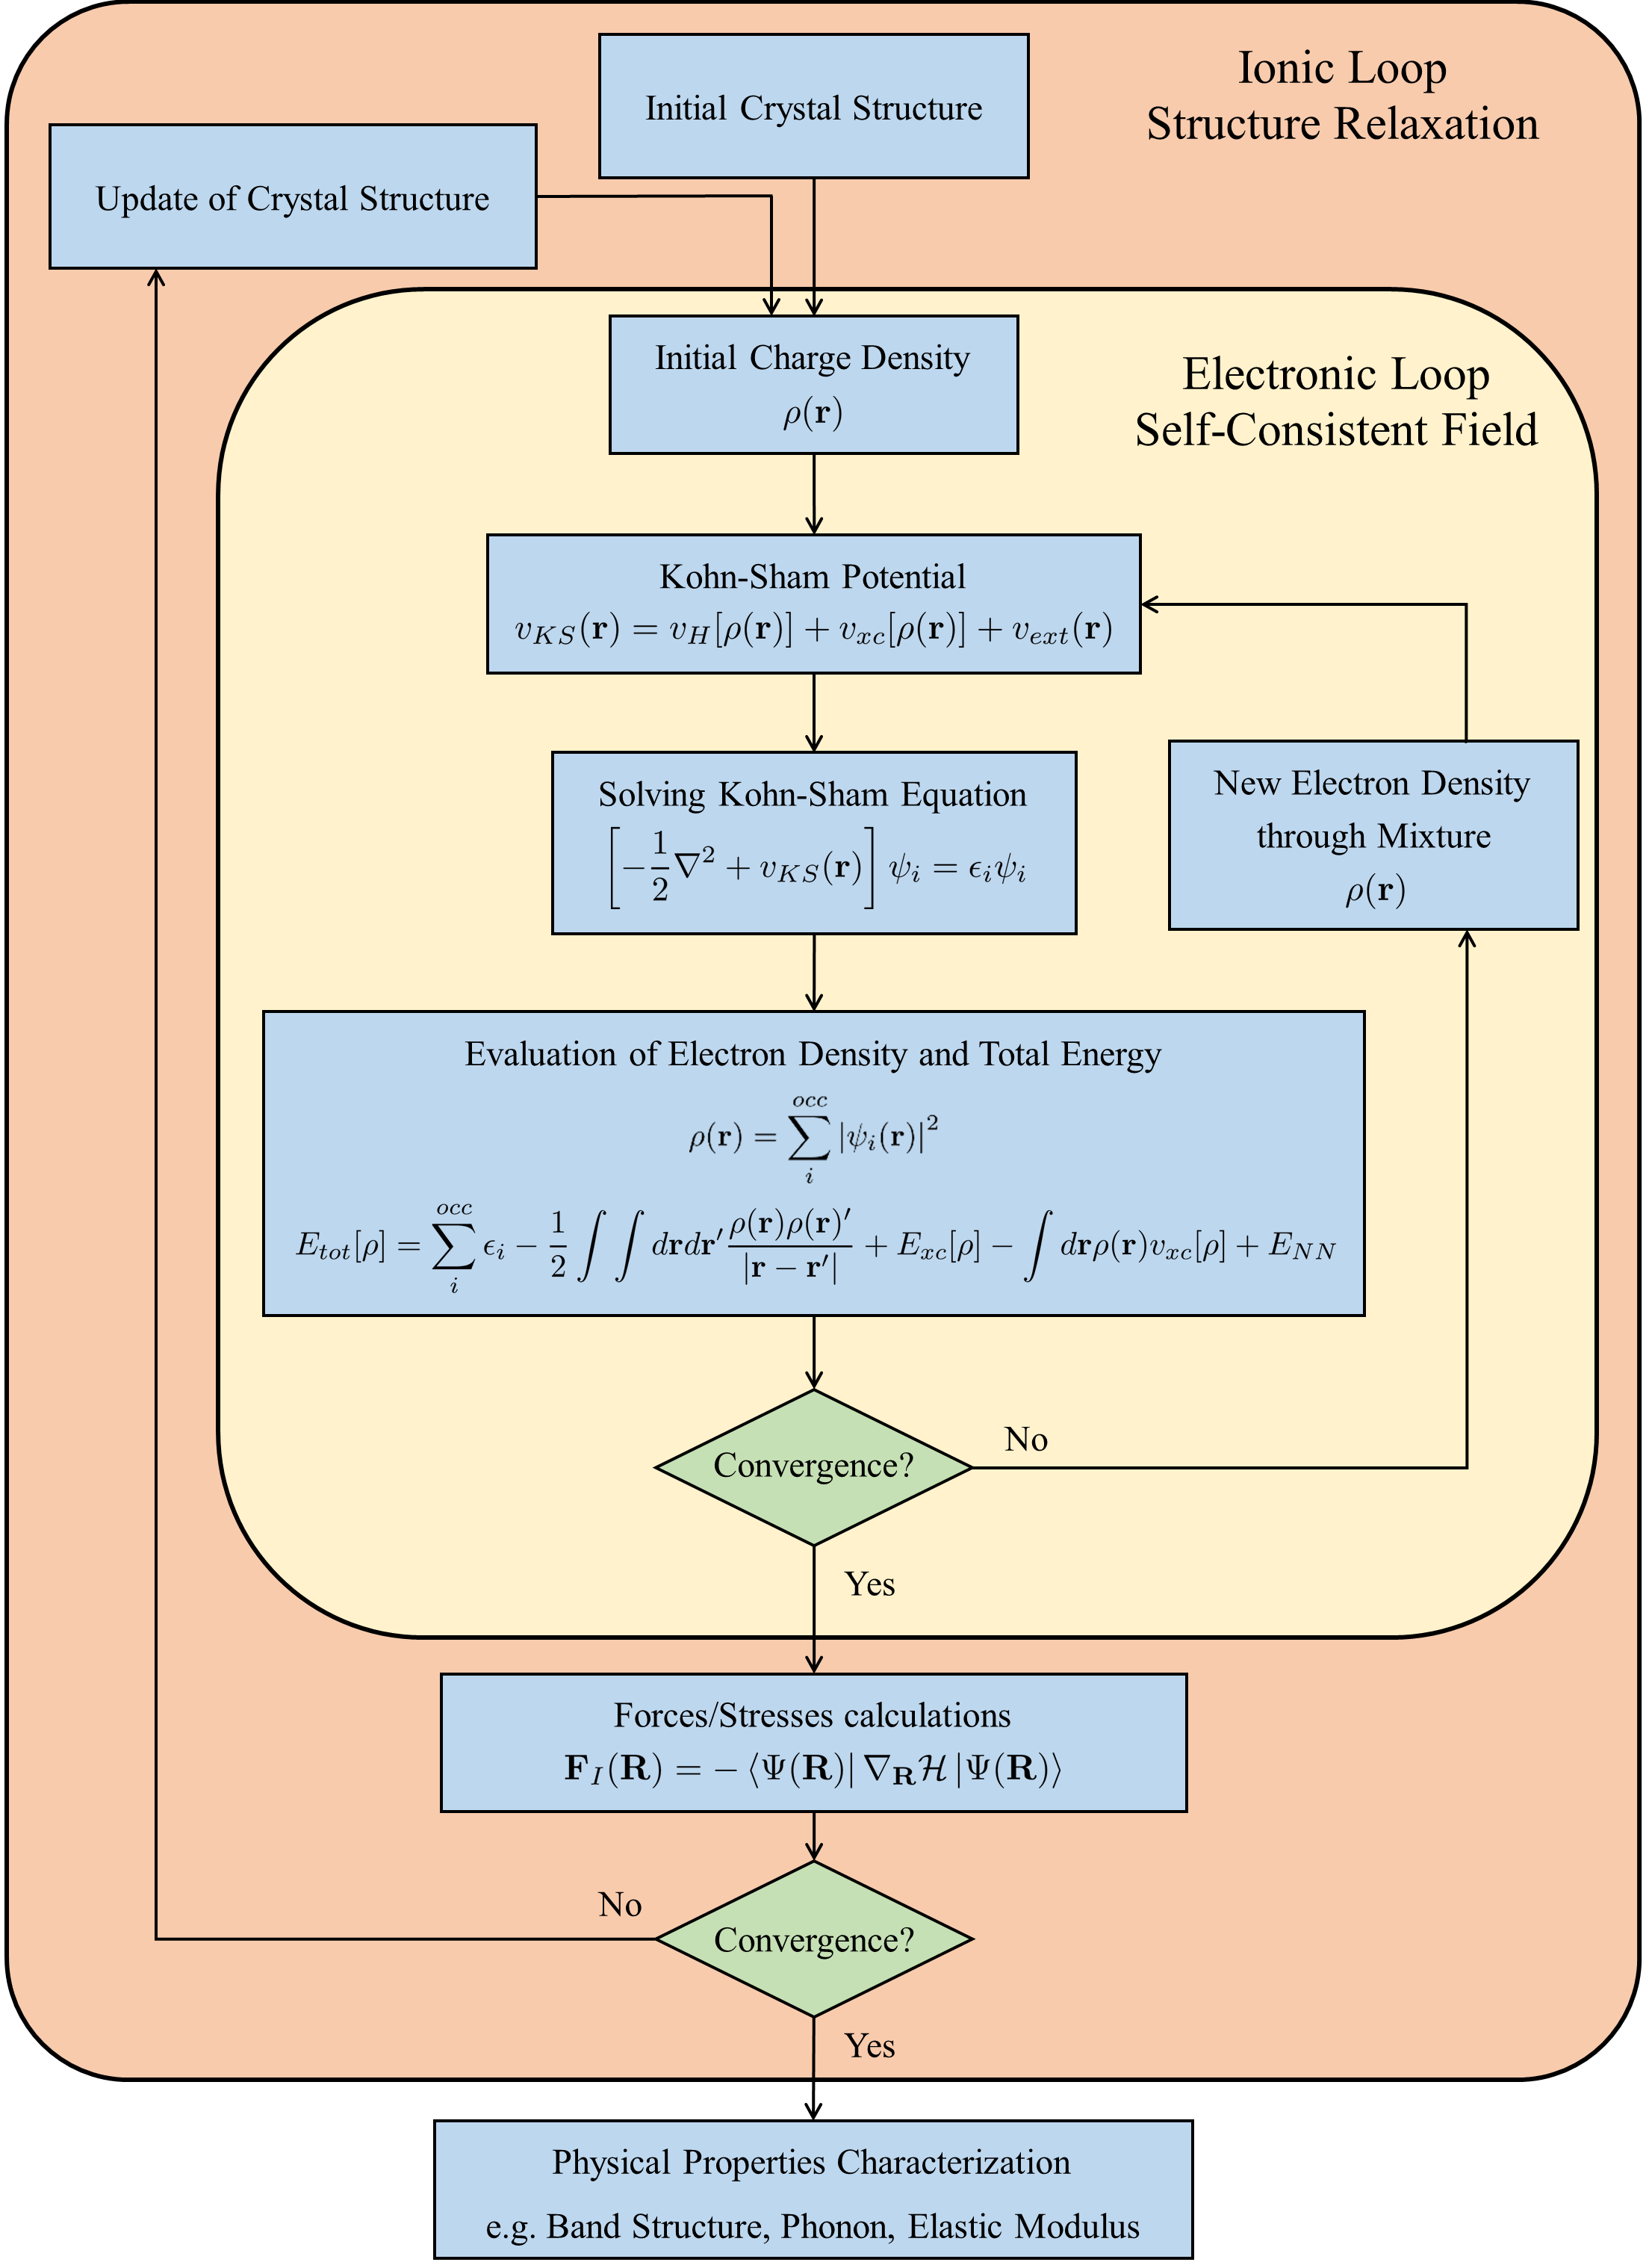
\includegraphics[width=1.0\textwidth]{DFT_flowchart.png}
        \caption[Flowchart of density functional theory calculations.]{Flowchart of density functional theory calculations including the ionic loop (outer loop) for crystal structure relaxation and electronic loop (inner loop) for self-consistent field.}
        \label{fig:DFT_flowchart}
    \end{figure}

\pagebreak




    %\subsection*{Evolutionary Algorithm}
    \addcontentsline{toc}{subsection}{Crystal Structure Prediction and Evolutionary Algorithm}
	{\centering
		\vspace{12pt} Crystal Structure Prediction and Evolutionary Algorithm
	    \par
	}
The crystal structure, the arrangement of compositional atoms, in a piece of material is the most important information that determines arguably all of the intrinsic physical properties of a material. With the information of crystal structure, one can compute several properties related to electronics, thermodynamics, vibration, optics, and magnetism through first-principles calculations like DFT. This allows researchers to search for materials with desired properties before conducting experiments like material syntheses and measurements. In certain situations, theoretical results might be the only way that one can resort to. For example, investigating materials at condition that cannot be approached by current experimental tools like extremely high pressure research. However, to obtain the crystal structure of a material fully by theoretical and computational tools is still a challenging task today, which is known as crystal structure prediction (CSP) \cite{oganov2011modern}.

The goal of CSP is to search for stable or metastable structures by exploring the gigantic configuration space of high-dimensional potential-energy surface (PES) with the knowledge of chemical compositions only. In the generic case, CSP is an optimization problem to locate the global or local minima in the Gibbs free energy landscape. The Gibbs free energy ($G$) is defined as
	\begin{equation}
		\label{eq}
		\begin{aligned}
			G = E_{tot} + PV - TS,
		\end{aligned}
	\end{equation}
where $E_{tot}$ is the total energy, $P$ is the pressure, $V$ is the volume, $T$ is the temperature, and $S$ is the entropy. Calculations for entropy involves heavy phonon calculations in solid systems, so in practice the enthalpy $H = E_{tot} + PV$ is considered as the fitness function to be minimized. With the progress of first-principles calculations, we can accurately estimate the enthalpy by DFT-based packages like VASP and \textsc{Quantum Espresso}. However, this optimization problem is challenging due to the facts of high dimensional configuration space and the huge number of local minimums when the number of atoms is large. We can estimate the difficulty of CSP problem by following the arguments in Ref. \cite{oganov2011evolutionary}. The total number of configuration is $C =  {V/\delta^3 \choose N} \prod_{i} {N \choose n_i}$ if not considering correlations between atoms. In this expression, $V$ is the volume, $\delta$ is the length-scale of the grid, $N = \sum_i n_i$ is the total number of atoms, and $n_i$ is the number of atom of $i$ type.


    \begin{figure}[htbp]
        \centering
        \captionsetup{singlelinecheck = false, justification=justified}
        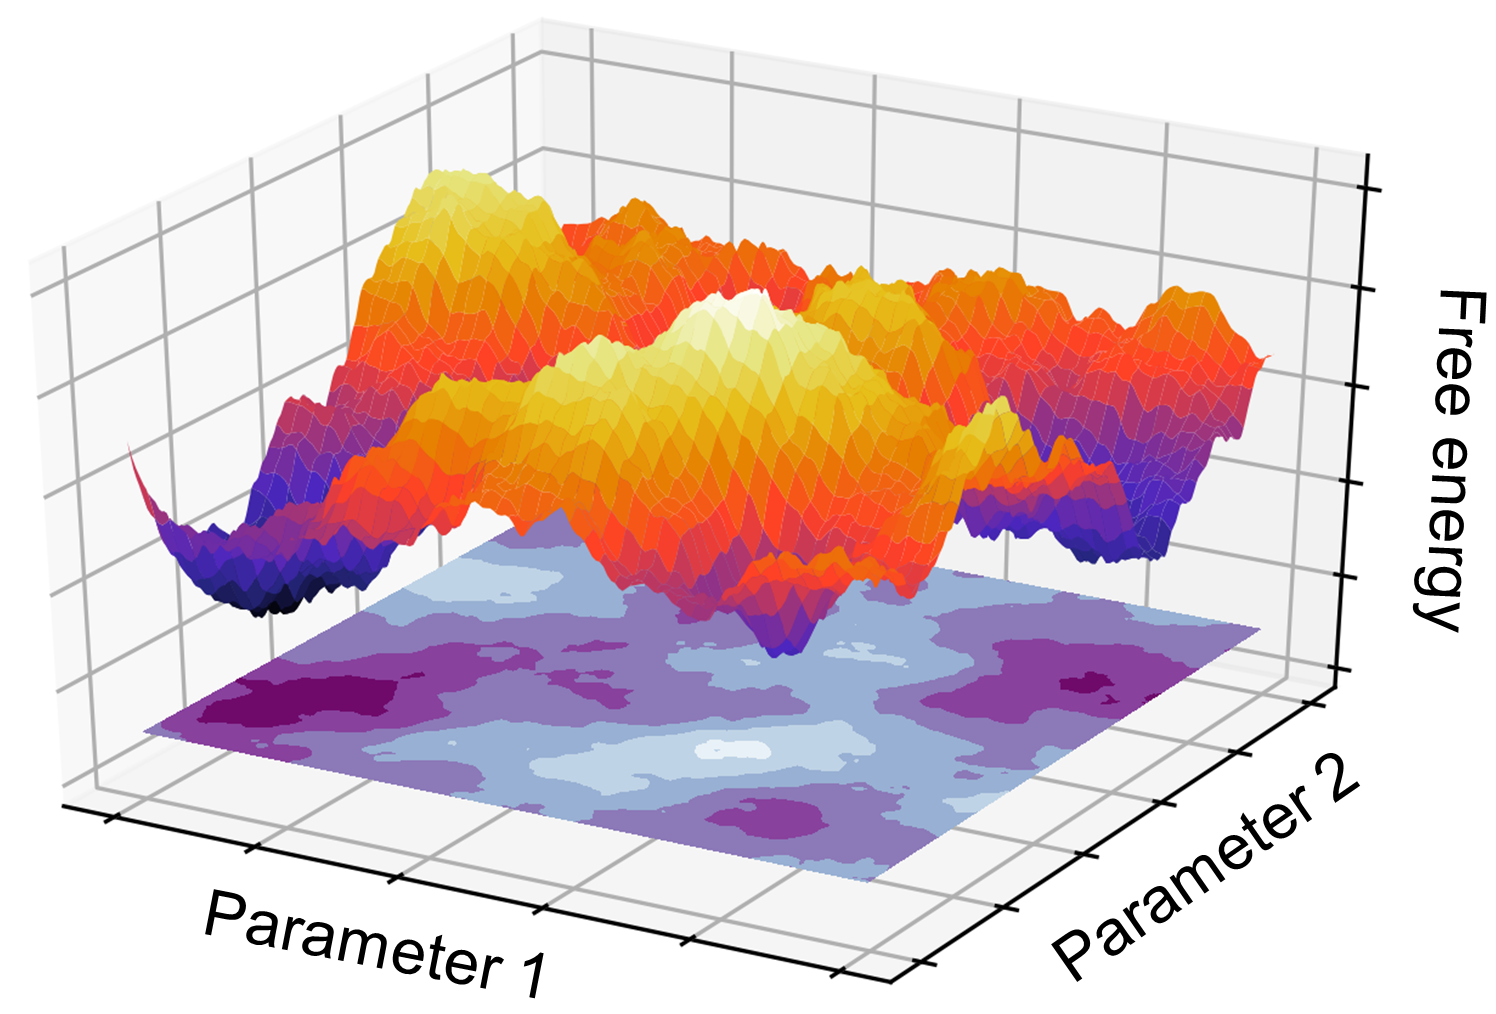
\includegraphics[width=0.70\textwidth]{free_energy_landscape.png}
        \caption{Schematic plot of free energy landscape.}
        \label{fig:landscape}
    \end{figure}

Besides, the dimensionality of the configuration space is $3N+6-3$ ($3N$ for atomic position, 6 for lattice geometry, 3 for the consideration of translational symmetry). To roughly estimate the number $C$, we consider a cubic box with a volume of 100 $\text{\normalfont\AA}^3$ that contains 10 atoms in two kinds, 5 for each. If we choose $\delta$ to be 1 $\text{\normalfont\AA}$, then what we are dealing with is an optimization process with 33 variables, and the total number of configuration is $\sim$ 1.1 $\times$ 10$^{18}$. In reality, we do not need to deal with such a huge phase space. Instead, this problem becomes searching for local minimums when we can take advantage of local optimization, which is the (local) structural relaxation built in modern DFT codes (see Fig. \ref{fig:DFT_flowchart}). The local optimization is usually based on methods like steepest-descent, conjugate-gradient, Broyden–Fletcher–Goldfarb–Shanno (BFGS) algorithm, etc. However, the number of local minimums also grows exponentially with increasing number of atoms.



To search for the local minimums efficiently, we need reliable global optimization algorithms to explore the configuration space. It is important to note that no method can guarantee to find the global minimum within a certain amount of time. Here we list some of popular global optimization algorithms: quasi-random, simulated annealing, meta-dynamics, minimum-hopping, particle swarm algorithm and evolutionary algorithm. In the following, we discuss the procedure of the method used in this dissertation -- evoultionary algorithm.


    \begin{figure}[htbp]
        \centering
        \captionsetup{singlelinecheck = false, justification=justified}
        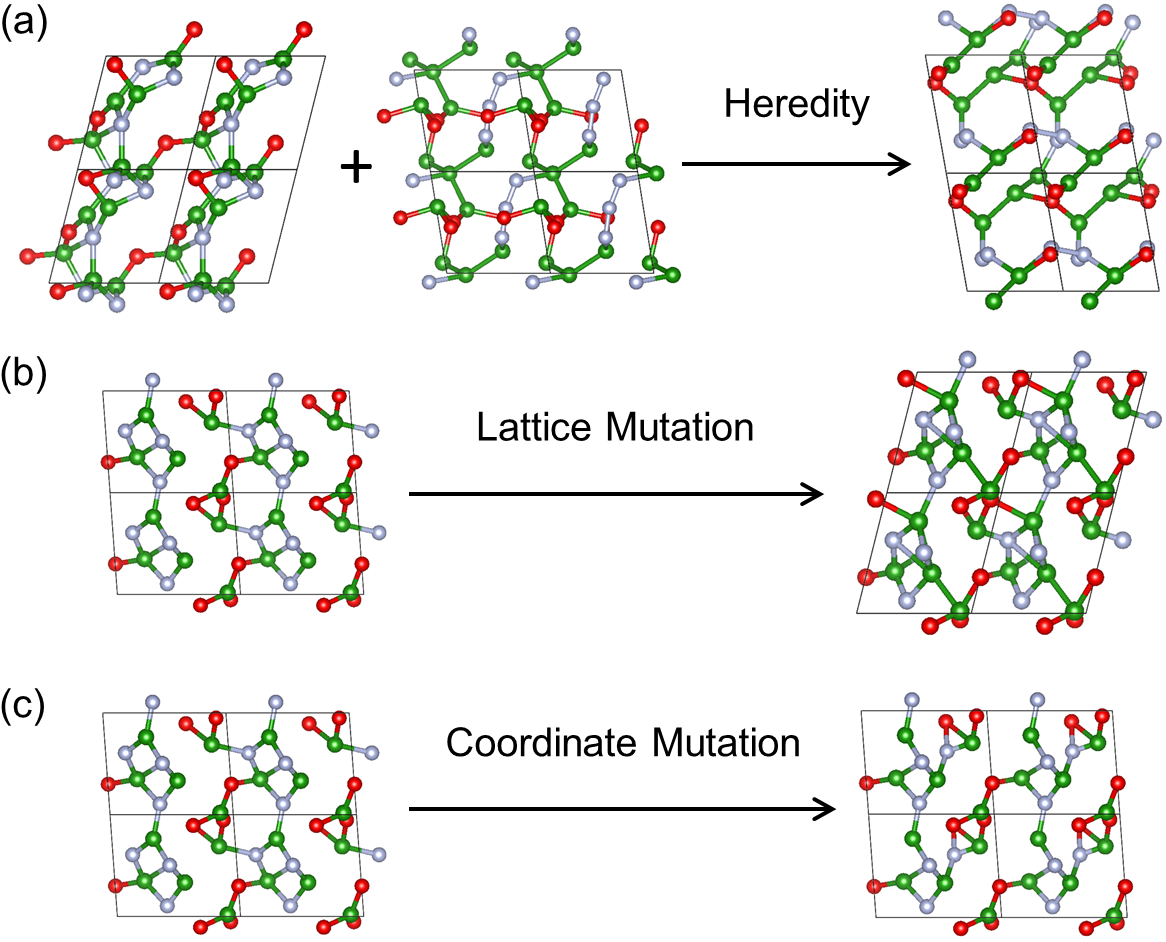
\includegraphics[width=0.8\textwidth]{operators.png}
        \caption[Examples of variation operators in evolutionary algorithm]{Examples of variation operators used to create new structures in the evolutionary algorithm for crystal structure prediction.}
        \label{fig:operators}
    \end{figure}

Evolutionary algorithm is a population-based optimization method aiming at finding the best solution in configuration space in a heuristic and also stochastic way. The process of evolutionary algorithm is inspired by the biological evolution, where the new generation can be created by operators like heredity or mutation. The heredity operator is also known as crossover operator or recombination, where a new candidate is a combination of two parts from its parents (one for each). In the context of crystal structure prediction, two sub-structures from parent structures are combined together to form a new structure. As for the mutation operator, it produces a new candidate from an old candidate in the population. The mutation operator can be lattice mutation or coordinate mutation that modifies an old structure by changing parts of structure variables. The heredity, lattice mutation, and coordinate mutation operators in crystal structure prediction can be found in Fig. \ref{fig:operators}.


Today, evolutionary algorithm packages for crystal structure prediction are usually combined with density functional theory to accurately evaluate the fitness function. In most of the cases, the fitness function is enthalpy, and the minimized enthalpy is corresponding to the thermodynamic favorable structure at a given pressure. Here, we describe the main steps in evolutionary algorithm:

{\vspace{16pt}}

{\it step 1:} Generating random structures

{\it step 2:} Local optimization and fitness evaluation for the first generation

{\it step 3:} Construction of initial population

{\it step 4:} Generating new structures through evolutionary operators.

{\it step 5:} Local optimization and fitness evaluation for new structures 

{\it step 6:} Iterating {\it step 4} and {\it step 5} until fulfilling the convergence criteria

{\vspace{16pt}}


    

The flowchart of evolutionary algorithm can be found in Fig. \ref{fig:EA_flowchart} .The fitness function can also be a physical property like the bulk modulus or dielectric constant, and the desired property can be optimized. However, such structures might not be thermodynamically stable in reality.


In this dissertation, we use \textsc{USPEX} (Universal Structure Predictor: Evolutionary Xtallography) package to carry out evolutionary searches in B-C-O and B-N-O systems. \textsc{USPEX}, designed by Oganov {\it et al.} \cite{oganov2006crystal, glass2006uspex, lyakhov2013new}, is an highly-efficient in crystal structure prediction, and its success is a result of carefully designed variation operators as well as efficient constraints that avoid unphysical and redundant structures in the search space. Besides, it also contains alternative methods including
random sampling, evolutionary metadynamics, and corrected particle swarm optimization algorithms. These alternative methods with evolutionary algorithm allow one to explore the search space in a more complete way.
In particular, evolutionary metadynamics is very powerful not only for global optimization and searching for low-energy metastable structures but also  predicting phase transition paths. In fact, this feature allows one to evaluate the energy barrier between two meta-stable structure, and therefore is highly-related to another important problem -- the synthesizability of a metastable structure.

    \begin{figure}[htbp]
        \centering
        \captionsetup{singlelinecheck = false, justification=justified}
        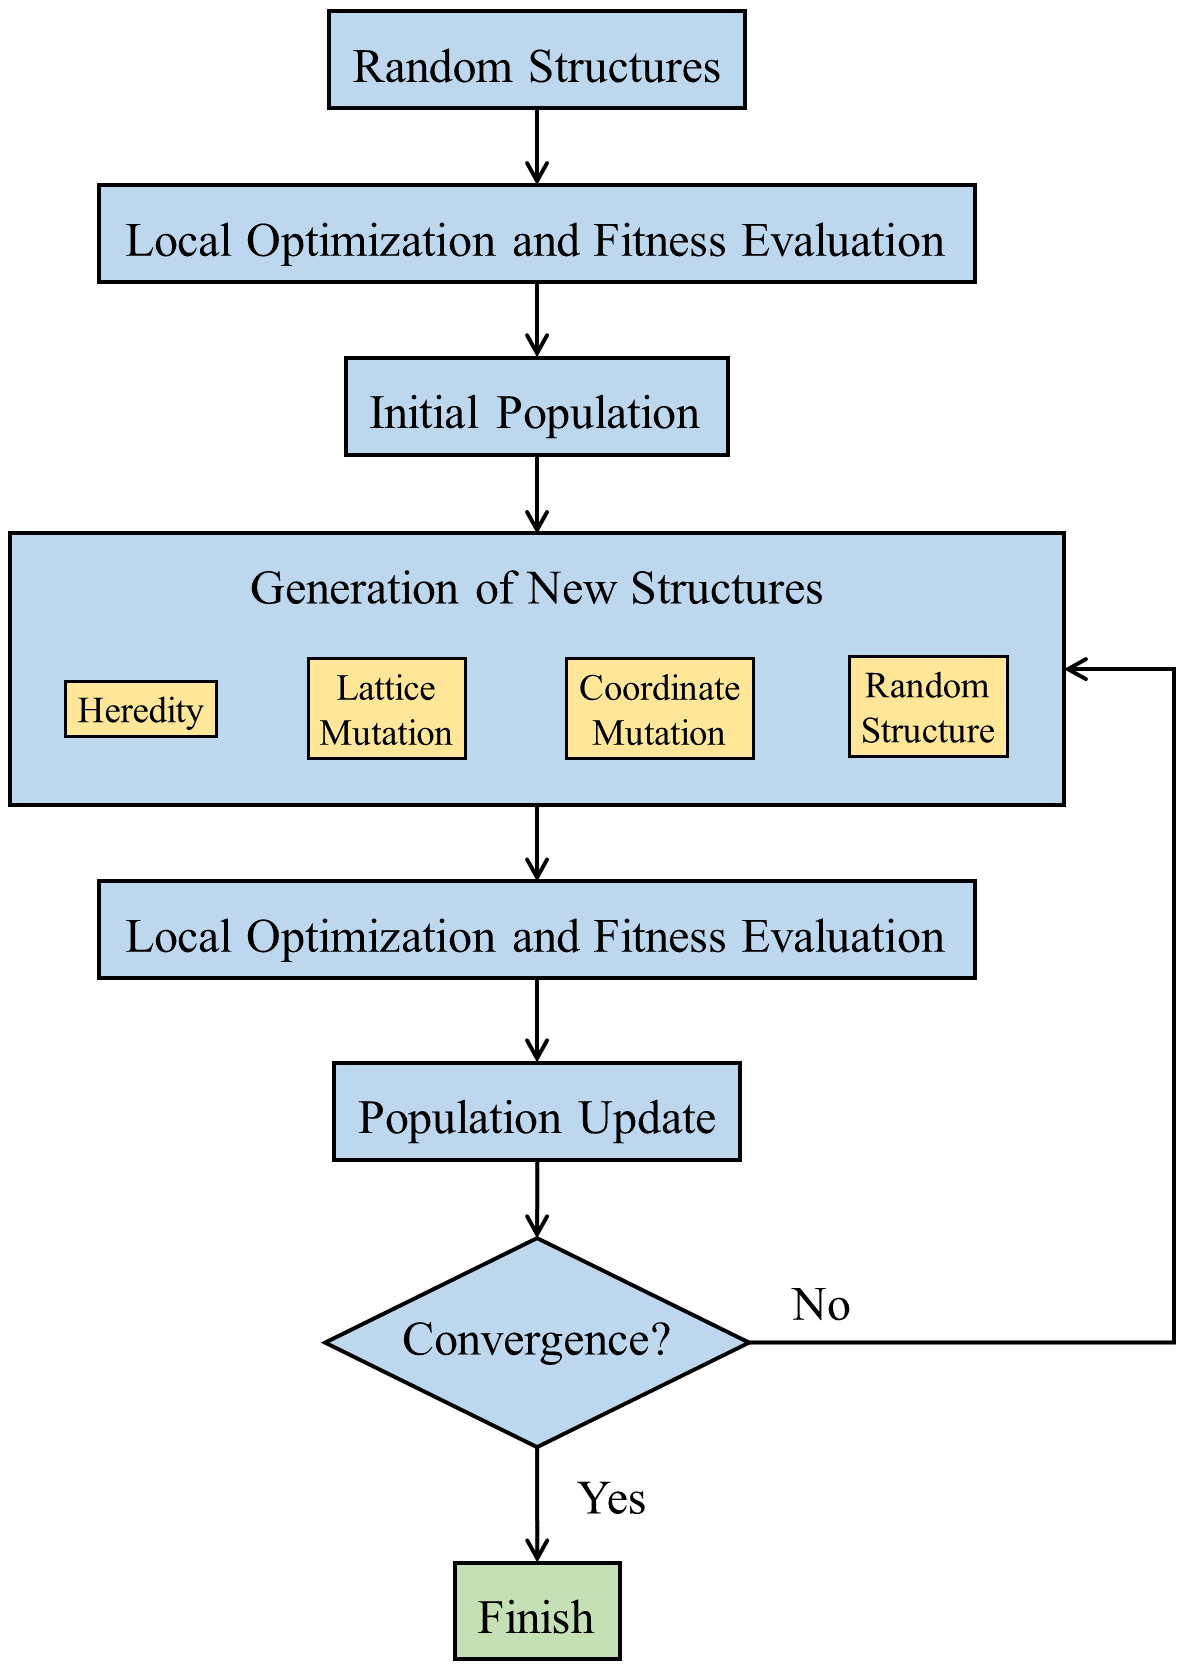
\includegraphics[width=0.65\textwidth]{EA_flowchart.png}
        \caption[Flowchart of evolutionary algorithm.]{Flowchart of evolutionary algorithm.}
        \label{fig:EA_flowchart}
    \end{figure}








    
    \pagebreak  

    %\subsection*{Machine Learning}
%    \addcontentsline{toc}{subsection}{Machine Learning}
%	{\centering
%		\vspace{12pt} Machine Learning
%	    \par
%	}
%The goal of machine learning is to find the best solution to a specific task by using existing data. There are three main categories in machine learning: supervised learning, unsupervised learning, and reinforcement learning. In supervised learning, data contains both features (or descriptor) and target (or label), and a supervised machine learning algorithm concerns finding the best mapping function from features to target using a portion of data known as training set. The obtained mapping function is a machine learning model that allows one to predict the unknown target as long as the corresponding features are given.

%In unsupervised learning, labels are not required in data, and the objective of unsupervised learning is to find patterns in unlabeled data. This is especially useful for cluster analysis.   





%   \pagebreak
    
    
    %\chapter{3 MACHINE LEARNING AND EVOLUTIONARY DISCOVERY OF TERNARY SUPERHARD MATERIALS}
    \addtocounter{numch}{1}
	\addcontentsline{toc}{chapter}{\hspace{0pt}  \the\value{numch} \hspace{-4pt} MACHINE LEARNING AND EVOLUTIONARY DISCOVERY OF \linebreak \hspace*{6pt} TERNARY SUPERHARD MATERIALS}
	{\centering
		\vspace{0pt} \hspace{0pt} \par
	}
	{\centering
		\vspace{56pt} CHAPTER  \the\value{numch}
	}
	{\centering\singlespacing
		MACHINE LEARNING AND EVOLUTIONARY DISCOVERY OF TERNARY SUPERHARD MATERIALS
	    \par
	}
	{\centering
		\vspace{0pt} \hspace{0pt} \par
	}
	
		
	
	
	
    %\subsection*{B-C-N Superhard Materials}
    \addcontentsline{toc}{subsection}{B-C-N Superhard Materials}
	{\centering
		\vspace{12pt} B-C-N Superhard Materials \\
	    \par
	}



	
	
	
		First-principles simulations based on density functional theory have played important roles in predicting new superhard compounds.
	However, {\it ab initio} methods are still computationally expensive and size-limited.
	On the other hand, data-driven approaches have proven to be powerful and efficient in exploring new materials~\cite{schmidt2019recent, zhou2019big, himanen2019data,chibani2020machine,saal2020machine,cai2020machine} -- thanks to recent advance in computing hardwares, development in machine learning algorithms, and availability of online materials database.
	For example, Meredig {\it et al.}~\cite{meredig2014combinatorial} have constructed a machine learning model to {\it screen over 1.6 million ternary compositions} and predicted 4,500 novel, potentially stable ternary materials.
	Therefore, data-driven machine learning approaches are promising for large-scale materials design and discovery.
	
	In principle, a machine learning framework can be implemented with different material features or descriptors for a wide range of target properties. Two popular properties to predict are bulk and shear moduli~\cite{furmanchuk2016predictive, de2016statistical, isayev2017universal, evans2017predicting,Mansouri2018, Avery2019}, which are also correlated with the material hardness.
	For example, de Jong {\it et al.}~\cite{de2016statistical} developed a technique based on gradient boosting and used features like the volume per atom and cohesive energy.
	Mansouri {\it et al.}~\cite{Mansouri2018} used support vector machines and combined elemental and structural properties as descriptors, where the cohesive energy was also identified as a crucial feature.
	These machine learning studies typically can achieve high prediction accuracy with only a few thousands of training data points. However, using cohesive energy, volume, melting point, crystal symmetry and so on as features may be less ideal, as obtaining these information for new compounds would require additional measurements or calculations.
	

	To explore the vast configuration space of ternary compounds, we develop random forests models to predict material mechanical properties, by using only features that can be derived directly from the chemical formula. The resulting machine learning models thereby can achieve large-scale prediction of new superhard and ultra incompressible materials for extreme environment applications.
	We also employ evolutionary structure prediction and density functional theory calculations to further validate the machine learning results.
	In particular, we propose three new superhard compositions -- BC$_{10}$N, B$_4$C$_5$N$_3$, and B$_2$C$_3$N -- and fully characterize their structural, phonon, and electronic properties. These new superhard compounds are all dynamically stable with relatively low formation energy, so they can potentially be synthesized by low-temperature plasma methods, {\it without the need of} high-temperature high-pressure conditions. It is noted that our newly suggested compound BC$_{10}$N has a computed hardness value $\sim 87$ GPa; once synthesized, the compound would become the second hardest material. Our computational flowchart is summarized in Fig. \ref{BCN_1_flowchart} and discussed in detail in the next section. 

	\begin{figure}[htbp]
        \centering
        \captionsetup{singlelinecheck = false, justification=justified}
        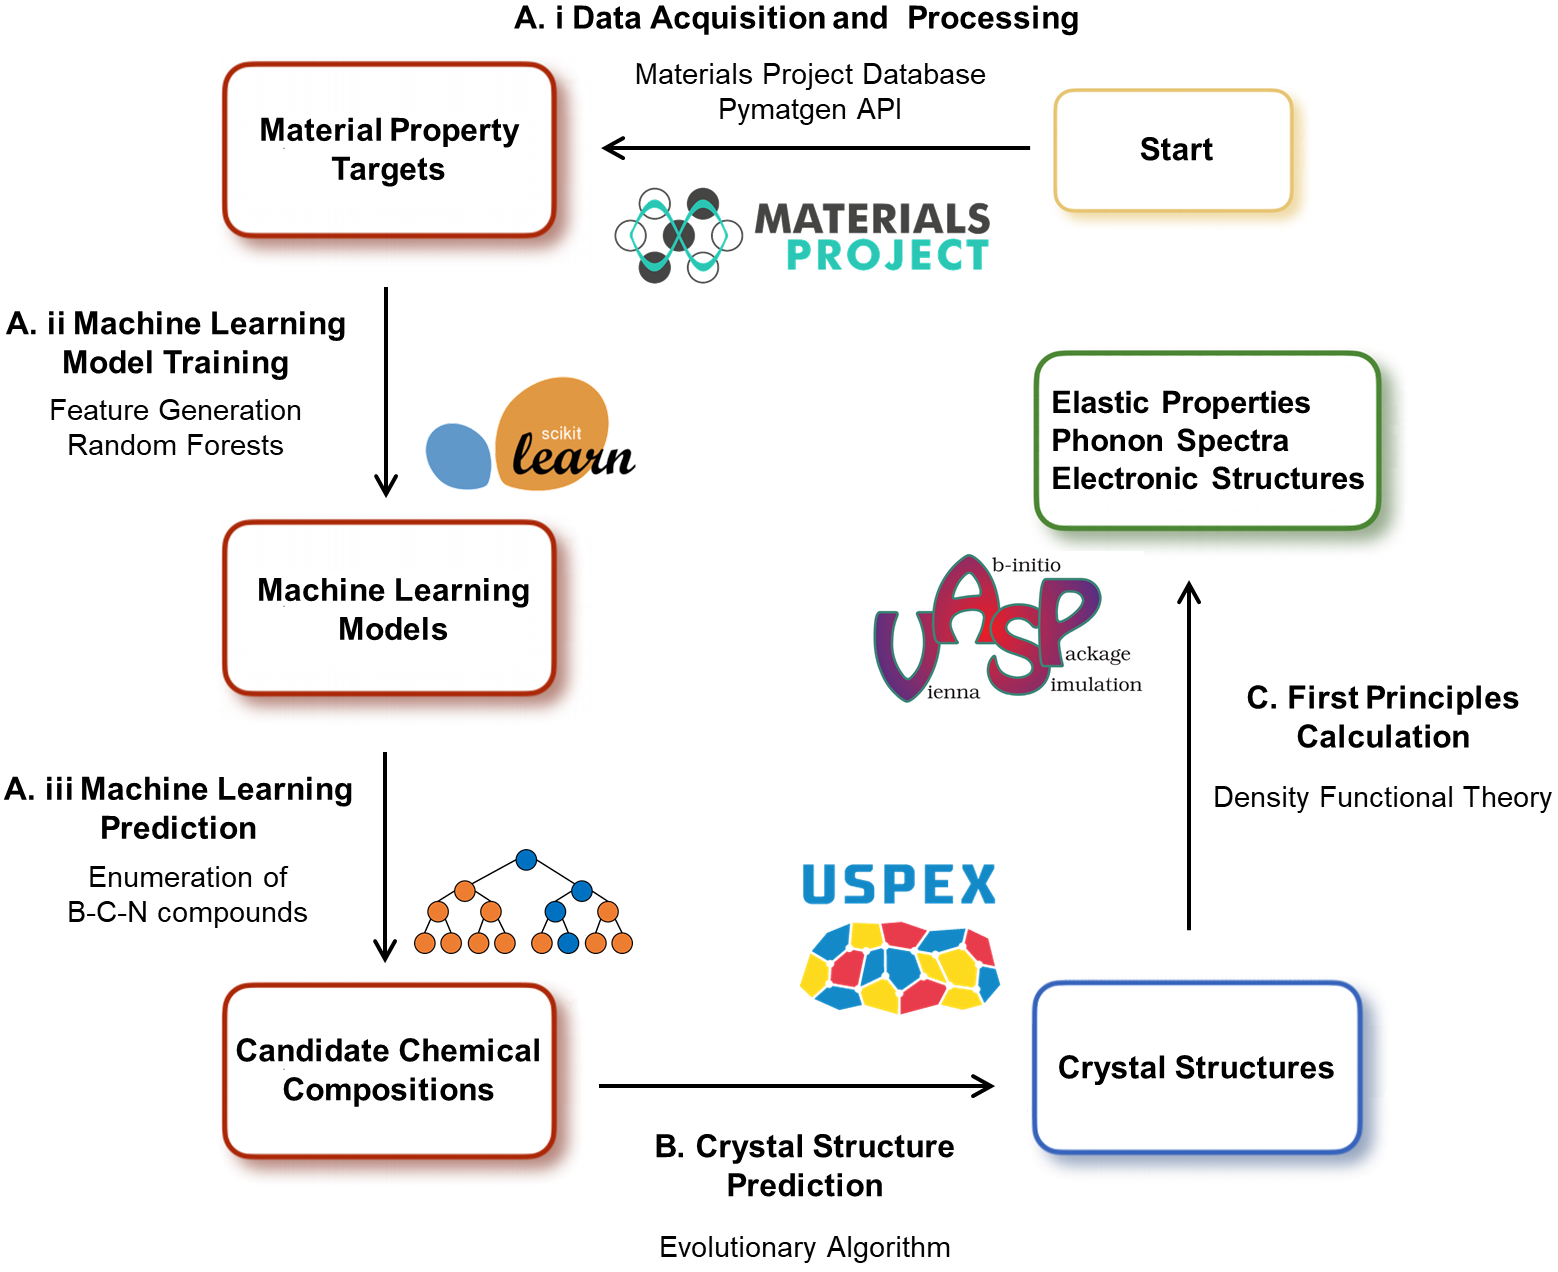
\includegraphics[width=1.0\textwidth]{BCN_1_flowchart.png}
        \caption[Computational flowchart for the B-C-N compounds.]{Computational flowchart of data-driven discovery of new superhard materials in our B-C-N study: {\bf A.i} Data acquisition and processing using the Materials Project~\cite{MP} database and its application programming interface (API) \textsc{Pymatgen}~\cite{PyMatGen}; {\bf A.ii} Machine learning model training with handcrafted features and regression algorithms implemented in the \textsc{scikit-learn} library~\cite{scikit-learn}; {\bf A.iii} Random forests prediction of chemical compositions for candidate superhard materials. {\bf B.} Crystal structure prediction of a given chemical formula using evolutionary algorithms implemented in the USPEX program~\cite{oganov2006crystal, glass2006uspex, lyakhov2013new}. {\bf C.} First-principles validation of the machine learning results with density functional theory calculations using the VASP software~\cite{kresse1996efficiency,kresse1996efficient}}
        \label{BCN_1_flowchart}
    \end{figure}


	
    	{\it Data acquisition --}
	There exist several online computational materials databases, such as AFLOW~\cite{aflow}, Materials Project~\cite{MP}, NOMAD Encyclopedia~\cite{nomad}, and the Open Quantum Materials Database (OQMD)~\cite{OQMD}. Here we use the Materials Project \cite{MP}, which provides open access to various computed properties of known and predicted crystalline compounds. The corresponding \textsc{Pymatgen}   (Python Materials Genomics) library \cite{PyMatGen} is utilized to extract the target properties of bulk modulus ($K$) and shear modulus ($G$).
	The Materials Project~\cite{MP} database also contains high-pressure phases and artificial crystal structures, which can exhibit extreme values of bulk and shear moduli. Therefore, we exclude those extreme outliers and focus on 10,421 selected compounds with $K$ and $G$ values both in the ranges of $0-550$ GPa.
	
	{\it Feature generation --} To build a supervised learning model using only chemical composition as input, we generate features (or descriptors) based on a compound's chemical formula. By following Ref. \cite{ward2016general}, we consider features related to stoichiometric attributes, elemental properties, orbital occupations, and ionic levels.
	Part of the features can be generated with the Python library \textsc{Matminer}~\cite{matminer}. 
	We {\emph{do not}} consider structural or electronic features like crystal symmetry, volume, melting point, band gap, etc. While including these additional features could improve the model performance, these information is {\textit {a priori}} unknown for new compounds. To expedite materials discovery, we thereby do not include features that require additional first-principles calculations.
	
	First, the stoichiometric features are $L^p$ norm $||x||_p = (\sum_i |x_i|^p)^{1/p}$, where $x_i$ is element $i$'s atomic fraction. These attributes capture the changes in atomic fraction, independent of the actual elements. As an example, the $p=2$ norm of Fe$_2$O$_3$ is $||x||_2 = \left((\frac{2}{5})^{2} + (\frac{3}{5})^2\right)^{1/2} \simeq 0.721$~\cite{ward2016general}. Here we consider 3 stoichiometric features, including the $p=0$ norm (i.e. the number of chemical components), and the $p=2, 3$ norms. The $p=1$ norm is equal to unity regardless of the chemical composition, so it is not considered. In addition, we do not find an apparent model improvement with more higher order norms ($p>3$), so they are not included.
	
	Second, the elemental features are computed using the minimum, maximum, and range for properties of each element present, as well as the values of fraction-weighted mean $\bar f = \sum_i x_i f_i$ and average deviation $\hat f = \sum_i | f_i - \bar f|$. Here, $f_i$ is the property of element $i$, and $x_i$ is the atomic fraction. We consider the following 10 properties: atomic number, atomic mass, element column number, row number, atomic radius, electronegativity, and the numbers of valence electrons in $s$, $p$, $d$, and $f$ orbitals, respectively. Therefore, there are 50 elemental-property features (= 5 values $\times$ 10 properties).
	Using again Fe$_2$O$_3$ as an example~\cite{ward2016general}, for the ``atomic number" property, $\bar f = \frac{2}{5}(26) + \frac{3}{5}(8) = 15.2$ and $\hat f = \frac{2}{5}|26 - 15.2| + \frac{3}{5}|8-15.2|= 8.64$. 
	
	Third, 4 orbital-occupation features are computed using the fraction-weighted average of the number of valance electrons respectively in $s$, $p$, $d$, and $f$ orbitals, divided by the fraction-weighted average of the total number of valance electrons. For example, Fe$_2$O$_3$'s $p$-orbital occupation feature is $F_p = \frac{2/5\times(0) + 3/5\times(4)}{2/5\times(8)+3/5\times(6)} \simeq 0.353$~\cite{ward2016general}.
	
	Finally, 3 features are based on ionic levels. The first is a Boolean number denoting whether it is possible to form a neutral ionic compound, by assuming that each element takes exactly one of its common charge states. The other two features are based on the ``ionic character'' of a chemical bond: $I(\chi_i, \chi_j)= 1- \exp( - (\chi_i-\chi_j)^2/4)$, where $\chi_i$ and $\chi_j$ are electronegativities for elements $i$ and $j$, respectively. In Pauling scale, fluorine has the highest electronegativity value of $\chi_F= 3.98$, and francium has the lowest electronegativity value of $\chi_{Fr} = 0.70$. The two features we consider are respectively the maximum ionic character $I$ between any two elements in a compound, and the mean ionic character $\bar I = \sum_{i,j} x_i x_j \chi_i \chi_j$.
	
	In total, 60 features are created. To simplify the training task, we do not consider additional feature engineering such as degree-2 polynomials, which otherwise could lead to thousands of new features and cause overfitting. The chemical compositions and their target properties of bulk and shear moduli for the 10,421 compounds considered here are written as a Python dictionary object saved in a \textsc{json} file. The features for all compounds are provided as a \textsc{csv} file accordingly. Both the data and our machine learning codes can be found in our github repository \cite{GitHub_Chen}.
	
	{\it Model training, validation, and application --} For regression task, we choose the random forests algorithm~\cite{ho1998, amit1997shape},
	which is a tree-based ensemble method. A random forests model builds multiple decision trees, by taking a random sample with replacement from the training set and a random subset of features to split tree nodes. The results averaged over individual trees serve as the final predictions, which help reduce variance and improve accuracy. However, without restriction on the tree depth, the model can become very deep and cause overfitting. Therefore, we constrain the pre-pruning parameter of tree depth to regularize the models.
	%our models constrain the pre-pruning parameter of tree depth to be between 5-15 layers.
	
	The model training is implemented with the \textsc{scikit-learn} library~\cite{scikit-learn}. We use 90$\%$ of our samples as the training and validation set, which is then used to determined the tree depth by 10-fold cross-validation. The remaining 10$\%$ is the test set used for an unbiased evaluation of the final model. We build two separate models to predict the bulk modulus ($K$) and shear modulus ($G$), respectively. We do not train a model for predicting the Vickers hardness ($H$), as the target hardness value is not as widely available as $K$ and $G$. On the other hand, there exist several empirical models for evaluating $H$~\cite{hardnessmodel2003,hardnessmodel2006,hardnessmodel2008,hardnessmodel2011,niu2019simple, mazhnik2019model}, based on physical properties such as bond length, bond strength, electronegativity, and covalent radius. Here we adopt hardness models that require only bulk and shear moduli as inputs~\cite{chen2011modeling, tian2012microscopic}, so that our regression results of $K$ and $G$ can be employed directly to predict $H$. 
	
	After training and evaluation, we apply the models to predict mechanical properties of B-C-N compounds and search for new superhard ternary materials. For candidate compositions identified with superhardness (i.e. $H \ge$ 40 GPa), we then perform crystal structure prediction and first-principles calculations to further validate the machine learning predictions.
	
	%\subsection{Crystal Structure Prediction}
	Crystal structure prediction (CSP) concerns finding the stable structure of a compound knowing only its chemical formula~\cite{wang2014perspective,graser2018machine, oganov2019structure}, and it requires an accurate and efficient estimation of the system's total energy $U$ (usually based on density functional theory), and an efficient optimization technique. Here we utilize the highly efficient implementation of evolutionary algorithm in USPEX package ~\cite{oganov2006crystal, glass2006uspex, lyakhov2013new}. In USPEX, several features have been added for the enhancement of searching efficiency. For example, USPEX implements	efficient constraint techniques being able to neglect unphysical and redundant regions in the search space. In our calculations, we examine over at least 1,000 structures for a given composition.	The first generation of structures are randomly created. Subsequent generations are created with $20\%$ from random structures and $80\%$ from heredity, softmutation, and transmutation operators.
	
	%\subsection{First-Principles Calculation}
	Our first-principles density functional theory (DFT) calculations are performed with the Vienna Ab initio Simulation Package (VASP)~\cite{kresse1996efficiency,kresse1996efficient}.
	The Monkhorst-Pack sampling scheme~\cite{monkhorst1976special} is used with a $\Gamma$-centered $k$-point mesh of $21\times 21 \times 5$ (resolution = 0.02$\times$2$\pi$/$\text{\normalfont\AA}$) points in the Brillouin zone.
	The convergence criteria of self-consistent and structural relaxation calculations are set to 10$^{-6}$ eV/unit-cell and 10$^{-3}$ eV/$\text{\normalfont\AA}$, respectively.
	We adopt a plane wave energy cutoff of 520 eV, which is sufficient to converge the DFT total energy difference $< 10^{-4}$ eV/atom.
	For each crystal structure, we first fully relax the lattice parameters and atomic positions.
	After structure relaxation, we then compute the corresponding mechanical, electronic, and phonon properties.
	All calculations use projector augmented wave (PAW)~\cite{PAW_1, PAW_2} pseudopotentials and the Perdew-Burke-Ernzerhof generalized gradient approximation (GGA) functional~\cite{perdew1996generalized}.

	\begin{figure*}[htbp!]
        \centering
        \captionsetup{singlelinecheck = false, justification=justified}
        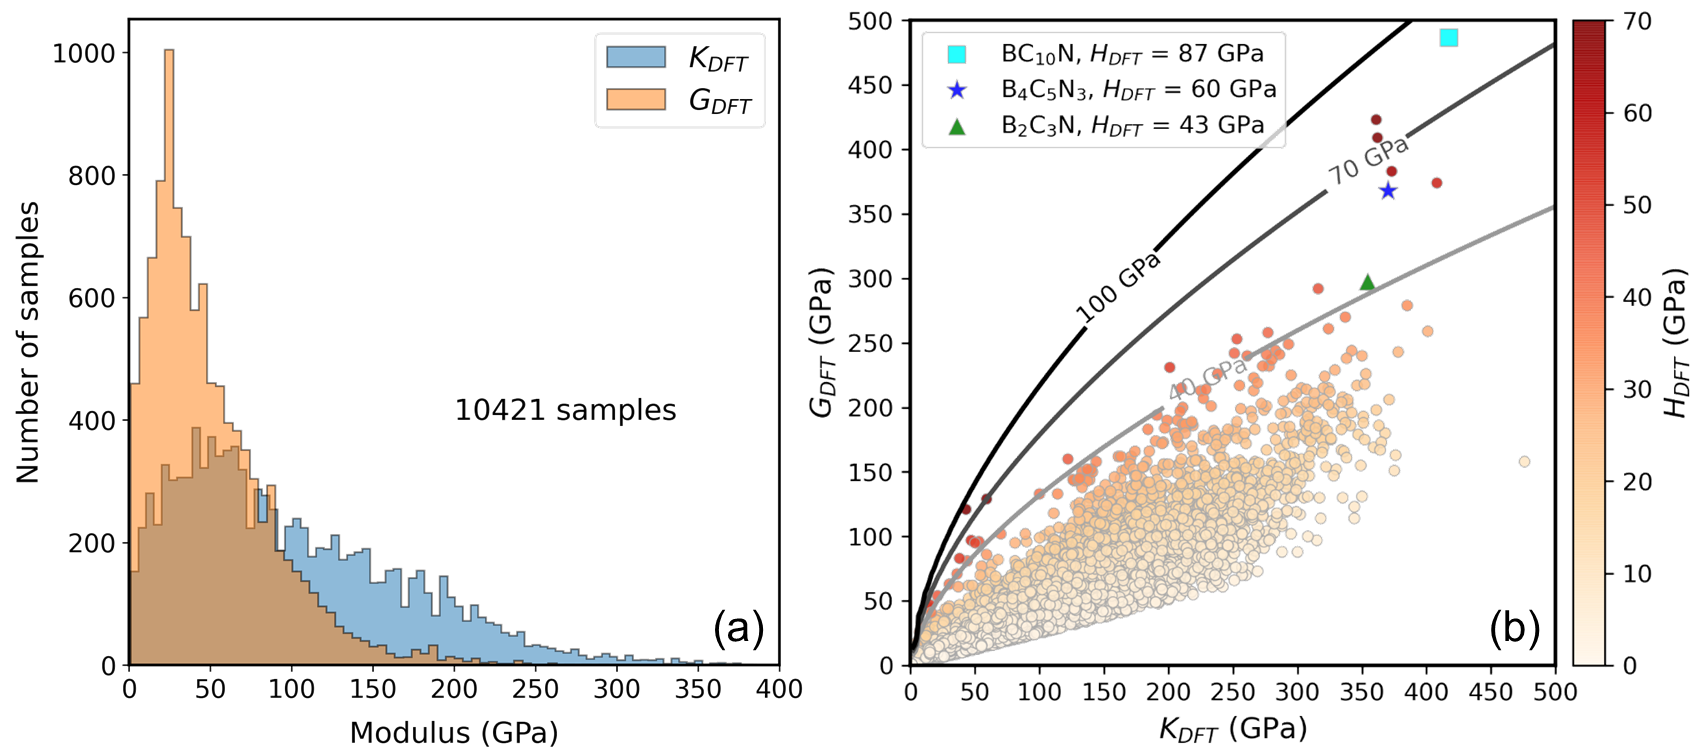
\includegraphics[width=1.0\textwidth]{BCN_2_data.png}
        \caption[Data distribution of bulk and shear moduli for B-C-N systems.]{(a) Histogram and (b) scatter plot of bulk ($K$) and shear ($G$) moduli for 10,421 samples acquired from the Materials Project~\cite{MP} database based on density functional theory (DFT) calculations. In (b), the false-color intensity represents the Vickers hardness ($H$) computed by Tian's empirical model using $K$ and $G$ as inputs. The solid curves represent the hardness contours using Tian's model~\cite{tian2012microscopic}.
		These contour lines can help quickly locate compounds with superhardness, with the caveat that the model's applicability might be more limited in the low-bulk/low-shear modulus region.
		The three newly proposed superhard compounds BC$_{10}$N, B$_4$C$_5$N$_3$, and B$_2$C$_3$N are highlighted respectively by the square, star, and triangle symbols.}
        \label{BCN_2_data}
    \end{figure*}
    
	
	We employ the strain-stress method~\cite{PhysRevB.65.104104} in VASP to compute the elastic constants $C_{ij}$,
	which in turn can determine the bulk and shear moduli using the Vogit-Reuss-Hill formula~\cite{voigt1928lehrbuch, reuss1929berechnung, hill1952elastic}.
	Phonon dispersion spectra are computed using the \textsc{Phonopy} package~\cite{phonopy}.
	Density functional perturbation theory with $2\times 2\times 1$ supercells are adopted to evaluate the second-order force constants. 
	
		%\section{Results and Discussion}
    

	Figure \ref{BCN_2_data} shows histograms of the bulk and shear moduli computed by DFT (denoted respectively as $K_{DFT}$ and $G_{DFT}$) for 10,421 samples acquired from the Materials Project database~\cite{MP}. Here, the DFT modulus values represent the Voigt-Reuss-Hill average moduli~\cite{voigt1928lehrbuch, reuss1929berechnung, hill1952elastic}, and the medians of $K_{DFT}$ and $G_{DFT}$ in Fig. \ref{BCN_2_data}(a) are 84 GPa and 40 GPa, respectively. Since the accuracy and applicability of a machine learning model largely depend on the training data, we have set a few criteria to select suitable samples during data acquisition.
	
	First, we have excluded sample materials with a formation energy $\ge 0.2$ eV/atom, as they are thermodynamically unfavorable.
	Second, we have neglected samples whose Voigt and Reuss modulus values differ by more than 50 GPa; this class of samples are typically layered quasi-two-dimensional materials, like graphite or hexagonal boron nitride, which are not the focus of our study.
	Third, we have utilized the Pugh's ratio $k$ $(\equiv G/K)$~\cite{Pugh} to further filter out materials with $k < 0.25$ due to their extremely small hardness, as well as materials with $k > 4.0$, which represents an extreme high-hardness structure (with $H > 200$ GPa) usually computed under high pressure.
	With these selection criteria, there are in total 10,421 samples considered in our machine learning study.
	
	Figure \ref{BCN_2_data}(b) shows the scatter plot for the distribution of bulk and shear moduli. The false-color intensity represents the corresponding material hardness ($H$), which is calculated by using Tian's empirical model~\cite{tian2012microscopic}:
	\begin{equation}
		\label{eq:Tian}
		\begin{aligned}
			H_V = 0.92k^{1.137}G^{0.708}.
		\end{aligned}
	\end{equation}
	This empirical formula dictates that superhardness requires a large Pugh's ratio $k$ and/or a high shear modulus $G$.
	Using Tian's model, we also plot hardness contour lines in Fig. \ref{BCN_2_data}(b). Materials in the contour region between $H= 40 - 100$ GPa are mostly compounds like C, BC$_2$N, c-BN, and M$_x$B$_y$ (M: Be or transition metal). The three newly proposed superhard ternary compounds -- BC$_{10}$N, B$_4$C$_5$N$_3$, and B$_2$C$_3$N -- are highlighted respectively by the square, star, and triangle symbols in Fig. \ref{BCN_2_data}(b). These materials will be discussed later in the paper.

	After data acquisition, we split the whole data into the training-validation set (90\%) and the test set (10\%). The training-validation set is used for grid search with 10-fold cross validation to search for a proper tree depth of the random forests models. We find that a maximum depth of 12 layers (with 100 estimators) is reasonable for obtaining a good balance between bias and variance.
	A deeper tree would not improve the model performance.
	After deciding on the maximum tree depth, we also utilize the training-validation set to further refine the machine learning models. 
	For an unbiased evaluation of the final model performance, we use the test set and consider the metric of Pearson correlation coefficient $r$:
	\begin{equation}
		\label{eq:3}
		\begin{aligned}
			r =
			\frac{ \sum_{i=1}^{n}(x_i-\bar{x})(y_i-\bar{y}) }{
				\sqrt{\sum_{i=1}^{n}(x_i-\bar{x})^2}\sqrt{\sum_{i=1}^{n}(y_i-\bar{y})^2}}.
		\end{aligned}
	\end{equation}
	Here, $x_i$ is the machine-learning predicted value for a single entry, and $y_i$ is the corresponding ``actual" value computed by DFT. $\bar{x}$ and $\bar{y}$ represent respectively the mean values of the predicted and the actual (DFT) values in the test set, which contains $n \sim 1,000$ sample points. The $r$ value can range between -1 to 1, and $r=1$ means that the prediction is 100\% accurate.
	\begin{figure}[htbp]
        \centering
        \captionsetup{singlelinecheck = false, justification=justified}
        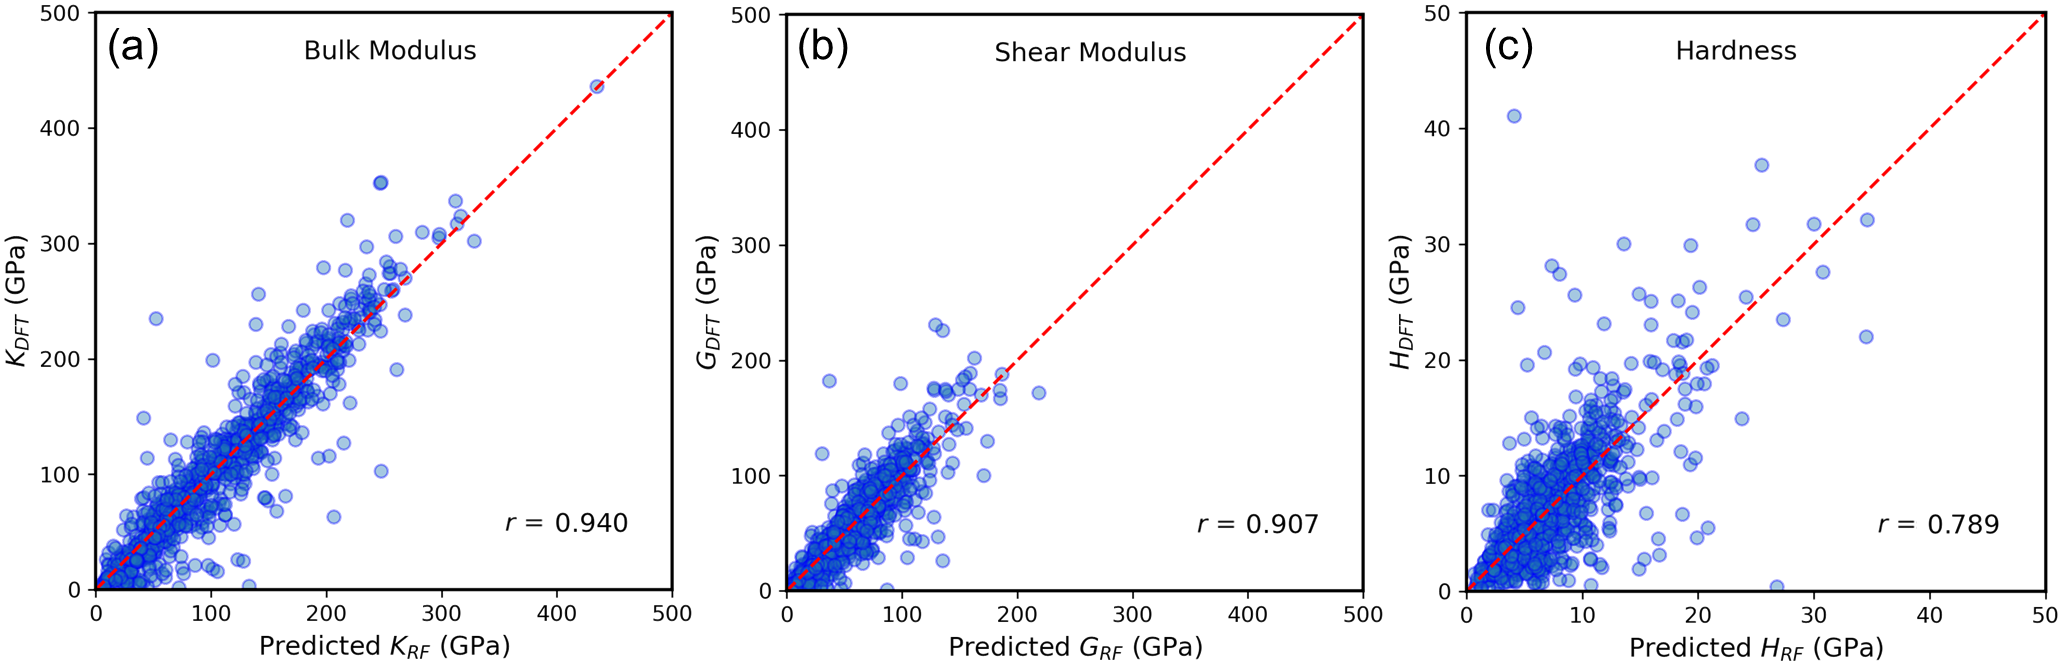
\includegraphics[width=1.0\textwidth]{BCN_3_model.png}
        \caption[Evaluation of random forests models in B-C-N study]{Evaluation of random forests (RF) models using the Pearson correlation coefficient ($r$) as a metric, for (a) bulk modulus ($K$), (b) shear modulus ($G$), and (c) hardness $(H)$. The machine learning models are trained to predict respectively $K$ and $G$, and both can achieve $r > 0.9$ when applied to the test set based on density functional theory (DFT) calculations. The predicted hardness $H_{RF}$ is obtained by using Tian's empirical formula with $K_{RF}$ and $G_{RF}$ as inputs, which results in an inferior correlation coefficient as anticipated.}
        \label{BCN_3_model}
    \end{figure}
    \pagebreak	
	Figure \ref{BCN_3_model} shows the $r$-value plots using the test set. For bulk and shear moduli [Fig. \ref{BCN_3_model}(a) and \ref{BCN_3_model}(b)], the data distribution follows closely the $r=1$ dashed line. The $r$ values of $K$ and $G$ are respectively 0.940 and 0.907 (, and their coefficients of determination $r^2$ are respectively 0.885 and 0.822). For the hardness $H_{RF}$ in Fig. \ref{BCN_3_model}(c), we note that the prediction is {\it not} obtained directly from a machine learning model. Instead, we use the machine learning predicted $K_{RF}$ and $G_{RF}$ with Tian's empirical formula in Eq. (1) to compute $H_{RF}$. Therefore, the data distribution in Fig. \ref{BCN_3_model}(c) is more dispersing with a $r$-value $\sim 0.79$, which is slightly inferior as expected.
	We also note that a higher $r$-value (or $r^2$ score) could be achieved by including additional features like volume, crystal symmetry, and cohesive energy, as done in previous studies~\cite{furmanchuk2016predictive, de2016statistical, isayev2017universal, evans2017predicting,Mansouri2018, Avery2019}. However, here we do not consider features that require additional measurements or calculations, but focus only on features that can be derived directly from the chemical formula, in order to achieve efficient large-scale materials discovery.
	
	Our machine learning models also provide information on feature importance to help reveal features that are more correlated with the bulk or shear moduli. Among the 60 features in our study, the atomic radius and $d$ electron occupation are the most important ones. 
	For example, the average atomic radius of a given compound and the bulk modulus exhibit a negative correlation with $r \sim -0.24$.
	Similarly, the $r$ value between the largest atomic radius and the bulk modulus is $r \sim -0.41$.
	The results indicate that in general, a smaller crystal unit cell will favor a higher bulk modulus.
	This is consistent with the facts that most superhard materials consist of light and small elements like Be, B, C, N, and O, and that diamond has the smallest volume per unit cell among all crystalline materials.
	On the other hand, the $d$ electron occupation rate is positively correlated with the bulk modulus, with a $r$ value $\sim 0.58$.
	This corresponds to the fact that many ultra incompressible materials are transition-metal borides like ReB$_2$ and Os$_2$B$_3$~\cite{Burrage_2020_ReB2,Burrage_2020_Os2B3}.
	
	With the random forest models, we can predict quickly the mechanical properties of a given chemical formula. Here we apply our models to ternary B-C-N compounds by enumerating a series of B$_x$C$_y$N$_z$ compositions, with $x,y,z\in \{1,2,3,...\}$.
	    
	\begin{figure}[htbp]
        \centering
        \captionsetup{singlelinecheck = false, justification=justified}
        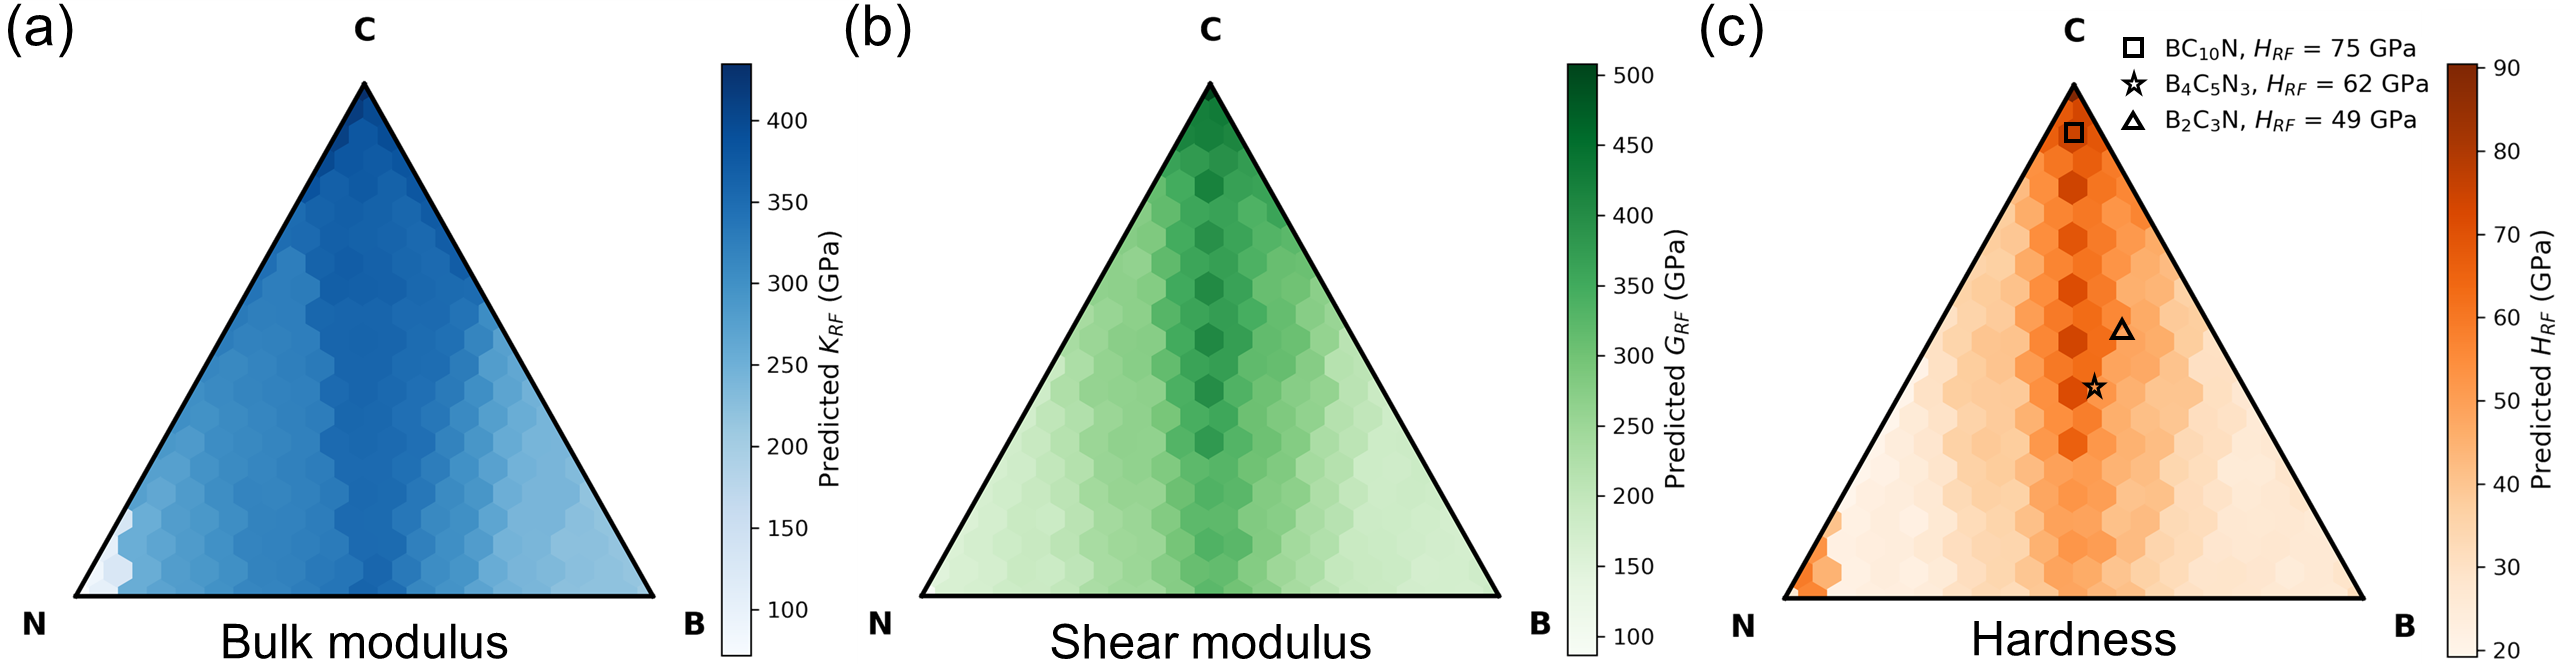
\includegraphics[width=1.0\textwidth]{BCN_4_prediction.png}
        \caption[B-C-N triangular plots for bulk modulus, shear modulus, and hardness]{Triangular (or ternary) B-C-N graphs for (a) bulk modulus ($K$), (b) shear modulus ($G$), and (c) hardness $(H)$, predicted by random forests (RF) machine learning models. Panel (c) indicates that a 1:1 B-N composition ratio can lead to various superhard compounds such BC$_2$N ($H_{RF} = 74$ GPa) and BC$_4$N ($H_{RF}=65$ GPa). The hardness of three newly proposed superhard compounds, BC$_{10}$N, B$_4$C$_5$N$_3$, and B$_2$C$_3$N are consistent with the DFT results. The triangular graphs are visualized by using the Python Ternary Plots library~\cite{pythonternary}.}
        \label{BCN_4_prediction}
    \end{figure}

	Figure \ref{BCN_4_prediction} shows the predicted triangular graphs,
	where the corner points correspond to unitary elemental compounds.
	For example, the pure boron phase in Fig. \ref{BCN_4_prediction}(c) is predicted to have $H_{RF}$ $\sim$ 30 GPa, which could be regarded as the hardness for $\alpha$-B, $\beta$-B, $\gamma$-B, or tetragonal B$_{52}$. For the pure carbon phase, the predicted $H_{RF} \sim 90$ GPa could be related to cubic or hexagonal diamond (lonsdaleite).
	One caveat is that the relatively high hardness predicted near the pure nitrogen phase may be unrealistic; this is due to small bulk moduli of nitrogen-dominated compounds, which leads to a large Pugh's ratio $k$ and a high hardness when Tian's model in Eq. (1) is used. If we implement more data selection rules by restricting the $K$ and $G$ values to be $>50$ GPa, then the artifact near the pure nitrogen phase could be avoided. However, this would cause overestimation in the overall mechanical properties.
	
	Figure \ref{BCN_4_prediction} also shows that B-C-N compositions with a $1:1$ B:N ratio can result in several superhard compounds with hardness $>60$ GPa. For example, the predicted hardness values of BC$_2$N and BC$_4$N by machine learning are 74 and 65 GPa, respectively. These predictions are consistent with previous experimental findings of superhardness in BC$_2$N (76 or 62 GPa)~\cite{solozhenko2001mechanical,BC2N_solozhenko2001synthesis,BC2N_zhao2002superhard} and BC$_4$N (68 GPa)~\cite{BC2N_zhao2002superhard}, which are synthesized under high-pressure and high-temperature conditions. 
    
	\begin{figure}[htbp]
        \centering
        \captionsetup{singlelinecheck = false, justification=justified}
        \includegraphics[width=1.0\textwidth]{BCN_5_dft.png}
        \caption[Crystal structures, band strcutures, and phonon dispersion of BC$_{10}$N, B$_4$C$_5$N$_3$, and B$_2$C$_3$N.]{Theoretical crystal structures (left panels), phonon dispersion spectra (middle panels), and electronic band structures (right panels) from evolutionary algorithm and density functional theory calculations for (a) BC$_{10}$N, (b) B$_4$C$_5$N$_3$, and (c) B$_2$C$_3$N. BC$_{10}$N is a wide-band-gap insulator, while B$_4$C$_5$N$_3$ and B$_2$C$_3$N are both metals. All three compounds are dynamically stable (i.e. without negative phonon modes). The crystal structures are visualized by the VESTA software~\cite{momma2011vesta}.}
        \label{BCN_5_dft}
    \end{figure}

    
	Motivated by the machine learning results in Fig. \ref{BCN_4_prediction}, we next employ evolutionary prediction with USPEX to search for potential superhard structures around the region with a B:N ratio $\sim$ 1:1. The calculations are performed under an applied pressure of 15 GPa to help locate stable structures of smaller volumes and larger hardness.
	We first consider 15 trial chemical formulae with even number of valence electrons, including BC$_3$N, BC$_5$N, BC$_6$N, BC$_3$N$_2$, B$_2$C$_3$N, B$_4$C$_5$N$_2$, etc., with a single-formula unit cell.
	However, most of the structures we found are graphite-like structures with $sp^2$ bonding, so they are not superhard.
	On the other hand, we find a diamond-like structure with $sp^3$ bonding for B$_2$C$_3$N [Fig. \ref{BCN_5_dft}(b)], which exhibits a hardness value $> 40$ GPa and a relatively low formation energy as discussed later.
	
	B$_2$C$_3$N is hexagonal with a superlattice structure along the (111) direction of cubic diamond. By comparing the $1\times 1 \times 2$ supercell of B$_2$C$_3$N (i.e. B$_4$C$_6$N$_2$), we find that such structure is similar to the $1\times 1 \times 2$ BC$_4$N~\cite{BC4N_Luo2008} (i.e. B$_2$C$_8$N$_2$) with 2 carbon atoms replaced by 2 boron atoms, or the structure of $1\times 1 \times 3$ BC$_2$N~\cite{BC2N_Liu2018} (i.e. B$_3$C$_6$N$_3$) with 1 nitrogen replaced by 1 boron. 
	In fact, such atomic replacement is also the case of boron-substituted diamond BC$_5$~\cite{PhysRevB.80.094106} ($H \sim 70$ GPa) in a 12-atom unit cell, with 2 carbon atoms replaced by 2 boron atoms. If one further replaces a carbon by boron in BC$_5$, the resulting B$_2$C$_4$ (BC$_2$)~\cite{Xu2010} structure is also superhard ($H \sim 56$ GPa). 
	Similarly, based on the 12-atom unit cell of diamond, the aforementioned superhard structure of BC$_2$N~\cite{BC2N_Liu2018} (BC$_4$N~\cite{BC4N_Luo2008}) also can be generated by replacing 6 (4) carbons with 3 (2) BN pairs.
	
	Using a 12-atom unit cell with a 1:1 B:N ratio, we first create the structure of BC$_{10}$N [Fig. \ref{BCN_5_dft} (a)] by replacing 2 carbon atoms in diamond by 1 pair of BN. Our random forests models predict that BC$_{10}$N has bulk and shear moduli equal to $K_{RF}=379$ GPa and $G_{RF}= 422$ GPa, respectively, which corresponds to a hardness $H_{RF}=75$ GPa by Tian's model.
	Using a similar rule, we also generate a new superhard composition B$_4$C$_5$N$_3$, by replacing 1 carbon with 1 boron in B$_3$C$_6$N$_3$.
	B$_4$C$_5$N$_3$ is predicted to have $K_{RF}=359$ GPa and $G_{RF}=369$ GPa, with $H_{RF}=62$ GPa.
	Other superhard B-C-N compounds also could be generated in a similar way. For example, B$_3$C$_7$N$_2$ and B$_2$C$_9$N could be obtained respectively from B$_3$C$_6$N$_3$ and B$_2$C$_8$N$_2$ by atomic substitution.
	Before we shift the focus to first-principles DFT validation of machine learning results, some comments are in order:
	(i) We have considered boron substitution in a 8-atom unit cell of BC$_2$N (i.e. B$_2$C$_4$N$_2$) to obtain B$_3$C$_3$N$_2$. However, we find that B-C-N compounds in a 8-atom unit cell have higher formation energies $>$ 300 meV/atom, which is consistent with early study on BC$_2$N by Chen {\it et al.}~\cite{PhysRevLett.98.015502}. (ii) We did not consider nitrogen substitution, because such structures tend to be thermodynamically more unstable.
	
		We next discuss DFT calculations of three new superhard B-C-N phases predicted by machine learning: BC$_{10}$N, B$_4$C$_5$N$_3$, and B$_2$C$_3$N.
	The structure of B$_2$C$_3$N [Fig. \ref{BCN_5_dft}(c)] is discovered by USPEX using a 6-atom unit cell. For BC$_{10}$N [Fig. \ref{BCN_5_dft}(a)] and B$_4$C$_5$N$_3$ [Fig. \ref{BCN_5_dft}(b)], they are generated by using the aforementioned rule of atomic substitution in a 12-atom diamond unit cell. We have performed additional USPEX calculations for BC$_{10}$N and B$_4$C$_5$N$_3$, but did not find any lower enthalpy structure.
	The structures in Fig. \ref{BCN_5_dft} can be treated as superlattices along the (111) direction of cubic diamond. All structures are trigonal systems with the hexagonal lattice space group $P3m1$ (No. 156), which has 6 independent elastic constants $C_{ij}$: $C_{11}$, $C_{12}$, $C_{13}$, $C_{14}$, $C_{33}$, $C_{44}$, ($C_{66}$ = $(C_{11}-C_{12})/2$). There are 4 necessary and sufficient mechanical stability conditions based on Born's criteria~\cite{PhysRevB.90.224104}: $C_{11} > C_{12}$, $C_{44} > 0$, $C_{13}^2  < \frac{1}{2}C_{33}(C_{11}+C_{12})$, and $C_{14}^2 < \frac{1}{2}C_{44}(C_{11}-C_{12})$.
	The three structures in Fig. \ref{BCN_5_dft} all fulfill these criteria, so they are mechanically stable.
	
    \begingroup
	\setlength{\tabcolsep}{6pt} % Default value: 6pt
	\renewcommand{\arraystretch}{1.5} % Default value: 1
	\begin{table*}[t]
		%  \begin{center}
		\caption[Mechanical  properties of newly-found superhard B-C-N compounds.]{Mechanical properties calculated by density functional theory (DFT), including density $\rho$ (atom/$\text{\normalfont\AA}^3$), bulk modulus $K$ (GPa), shear modulus $G$ (GPa), Young's modulus $E$ (GPa), Pugh's ratio $k$, Poisson's ratio $\nu$, universal elastic anisotropy $A^U$, hardness $H$ (GPa), and formation energy $\Delta$E (meV/atom).}
		\label{tab:table2}
		\begin{tabular}{l|c|c|c|c|c|c|c|c|c|c} % <-- Alignments: 1st column left, 2nd middle and 3rd right, with vertical lines in between
			Formula   & $\rho$ & $K$ & $G$ & $E$ & $k$ & $\nu$ & $A^U$ & $H_{RF}$ & $H_{DFT}$ & $\Delta$E\\
			%     $\alpha$ & $\beta$ & $\gamma$ \\
			\hline
			BC$_{10}$N   & 0.173 & 417  & 487 & 1052 & 1.166 & 0.080 & 0.058 & 75 & 87 & 79.5 \\
			B$_4$C$_5$N$_3$  & 0.166 & 370  & 368 & 829 & 0.995 & 0.125 & 0.221 & 62 & 60 & 141.3 \\
			B$_2$C$_3$N  & 0.164 & 354  & 298 & 697 & 0.840 & 0.172 & 0.792 & 49 & 43 & 155.9 \\
			diamond  & 0.175 & 432 & 518 & 1110 & 1.199 & 0.072 & 0.044 &90 & 94 & 0
		\end{tabular}
		%  \end{center}
	\end{table*}
	\endgroup
	
	
	Figure \ref{BCN_5_dft} middle panels show phonon spectra for the corresponding structures in the left panels, and all structures are dynamically stable without negative modes. Their phonon dispersions are fairly similar, due to the similarity in the crystal structures.
	Among them, BC$_{10}$N has the highest phonon frequency above 1250 cm$^{-1}$, while B$_4$C$_5$N$_3$ and B$_2$C$_3$N have slightly lower phonon frequencies near 1200 cm$^{-1}$ at the top of the phonon bands. 
	We note that cubic diamond has the highest phonon frequency above 1300 cm$^{-1}$. The results indicate that phonon bands are softened with increasing B/N content. This phonon softening is consistent with the phenomenon observed in boron-incorporated diamond BC$_5$~\cite{baker2018computational}.
	
	The electronic band structures are shown accordingly in Fig. \ref{BCN_5_dft} right panels. BC$_{10}$N exhibits a wide band gap $\sim$ 3.5 eV, so it is a superhard insulator. On the other hand, the electron-deficit B$_4$C$_5$N$_3$ and B$_2$C$_3$N are metals, where their valence band maximums are shifted towards the conduction bands. Due to the similarity of phonon and electronic dispersion relations between B$_4$C$_5$N$_3$/B$_2$C$_3$N and BC$_5$~\cite{baker2018computational,PhysRevB.80.094106, BC5_SC}, superconductivity may be observed in the predicted B$_4$C$_5$N$_3$ and B$_2$C$_3$N compounds as well. However, discussion related to superconducting properties is beyond the scope of this study. 
	
	The elastic constants $C_{ij}$ computed by DFT for the structures in Fig. \ref{BCN_5_dft} can be utilized to derive other mechanical properties, such as the bulk modulus ($K$), shear modulus ($G$), and Young's modulus ($E$). The Vicker's hardness $H$ also can be calculated by Eq.(1) with $K$ and $G$ as input. Details of the calculation results are given in Table \ref{tab:table2}
	Notably, BC$_{10}$N has supreme mechanical properties with a hardness of 87 GPa, which is comparable to diamond. Once synthesized, BC$_{10}$N would be the second known hardest material.
	
	Table I also indicates that when the B/N content increases, the mechanical \newline strengths like bulk and shear moduli as well as hardness will tend to decrease, which is consistent with the trend of phonon softening. The computed Cauchy pressures ($= C_{12}-C_{44}$)~\cite{PhysRevB.86.134106} of BC$_{10}$N, B$_4$C$_5$N$_3$, and B$_2$C$_3$N are all negative (and equal to -405 GPa, -209 GPa, and -121 GPa, respectively), which suggests their brittle properties and strong covalent bondings. 
	In addition, the Pugh's ratio ($k = G/K$)~\cite{Pugh} is greater than 0.571 for all three ternary compounds, indicative of their brittle properties as well. 
	By increasing the B/N content, other B-C-N compounds like B$_4$C$_5$N$_3$ and B$_2$C$_3$N can become more ductile.
	Table I also demonstrates that the density $\rho$ (atom/$\text{\normalfont\AA}^3$) is positively correlated with mechanical strength, while the poisson's ratio $\nu$ and universal elastic anisotropy $A^U$~\cite{Univ_Ela_Aniso} have negative correlations with elastic moduli and hardness.
	
	Finally, we evalulate the thermodynamic stability of the newly proposed B$_x$C$_y$N$_z$ compounds, by calculating the formation energy $\Delta E$ (also shown in Table \ref{tab:table2}):
	\begin{equation}
		\label{eq:5}
		\begin{aligned}
			\Delta E = \frac{E(B_xC_yN_z)-yE(C) - zE(BN) - (x-z)E(B)}{x+y+z},
		\end{aligned}
	\end{equation}
	which is the difference between the total energy $E$ of B$_x$C$_y$N$_z$ and the atomically weighted reference total energies $E$ of diamond, cubic BN, and $\alpha$-B. The formation energies of the three compounds are positive, which is consistent with previous study on BC$_2$N~\cite{PhysRevLett.98.015502}, suggesting that $\Delta E$ increases due to B-C and C-N bondings.
	Among the three proposed compositions, BC$_{10}$N has the least number of B-C and B-N bonds, and it has the lowest formation energy $<$ 100 meV/atom. Since $\Delta E$ of BC$_{10}$N is smaller than those of BC$_{2}$N and BC$_{4}$N, it is likely that BC$_{10}$N can be synthesized without extreme conditions~\cite{aykol2018thermodynamic}, using e.g. low-temperature plasma methods.
	
	To conclude this section, we have built random forest models to predict bulk and shear moduli by using target elastic properties in the Materials Project database~\cite{MP}.
	The machine learning models utilize only materials features that can be derived directly from a given chemical formula, so they are suitable for large-scale materials characterization and discovery. We have applied the resulting models to B-C-N compounds to search for new superhard ternary materials.
	The machine-learning predicted ternary graphs indicate that a 1:1 B:N ratio can lead to various promising superhard materials with hardness $>$ 40 GPa.
	We also have utilized evolutionary structure prediction together with first-principles density-functional-theory calculations to further validate the machine learning results.
	We have proposed three new potential superhard ternary compounds -- BC$_{10}$N, B$_4$C$_5$N$_3$, and B$_2$C$_3$N -- and fully characterized their properties. 
	In predicted ternary compounds, BC$_{10}$N is a wide band-gap semiconductor, while B$_4$C$_5$N$_3$ and B$_2$C$_3$N show metallic behavior. 
	Among them, BC$_{10}$N has a hardness value $\sim 87$ GPa and a relatively low formation energy. Therefore, BC$_{10}$N may be synthesized without high-pressure and high-temperature conditions, for example using low-temperature plasma methods.
	Once synthesized, BC$_{10}$N would become the second known hardest material with a wide range of potential applications in extreme environments.
	
	\vspace{12pt}
	
	\noindent This section is based on our study published in {\it npj Comput Mater} {\bf 7}, 114 (2021) \cite{chen2021machine}.





		

			
	
    
    \pagebreak
    %\subsection*{B-N-O Superhard Materials}
    \addcontentsline{toc}{subsection}{B-N-O Superhard Materials}
	{\centering
		\vspace{12pt} B-N-O Superhard Materials
	    \par
	}

B-N-O compounds have attracted considerable attention because it shows potential to several research areas including chemical adsorption \cite{shankar2021gas}, fluorescent dots \cite{ren2020boron}, water splitting \cite{xie2012boron}, wide bandgap insulator with large dielectric strength  \cite{arnold2021composition}, as well as electrochemical applications \cite{dussauze2013lithium}. Althoug the synthesized B-N-O compounds have several forms including amorphous, porous, layered, thin-film, and nano-particle, our knowledge to the mechanical properties of bulk B-N-O are still limited. Recently, Bhat {\it et al.} employed HPHT methods to synthesize crystalline novel B-N-O compounds with zinc-blende-like structure \cite{bhat2015high}. In their previous experiments for the synthesis of B-C-N compounds, they found the initial materials tended to decompose into diamond and c-BN. Moreover, they found some crystals contained considerable amount of oxygen as well as boron and nitrogen, which motivated their HPHT synthesis for B-N-O compounds. They used hexagonal BN and B$_2$O$_3$ in a ratio of 3 : 1 as the initial materials. Afterwards, the crystalline B-N-O material with composition ratio of 6:4:3 was synthesized under HPHT condition.

Besides, Bhat {\it et al.} also conducted crystal structure prediction and density functional theory characterization, their computaional resutls showed that the most stable structures contained ordered vacancies in zinc-blende type structure, and such structures have a high bulk modulus of 300 GPa, which indicates that B-N-O compounds might have superhardness \cite{bhat2015high}. Motivated by the experimental findings by Bhat {\it el al.}, here we again use evolutionary crystal structure prediction, random forests models, and density functional theory to search for new superhard materials in ternary B-N-O compounds. However, we found that the number of B-N-O data in Materials Project database is small, which reflects that crystalline B-N-O compounds are not fully explored. Moreover, the lack of relevant data might lead to inaccurate machine learning prediction. Therefore, here we adopt another study procedure based on the data generated from our evolutionary searches. 


    
	\begin{figure}[htbp]
        \centering
        \captionsetup{singlelinecheck = false, justification=justified}
        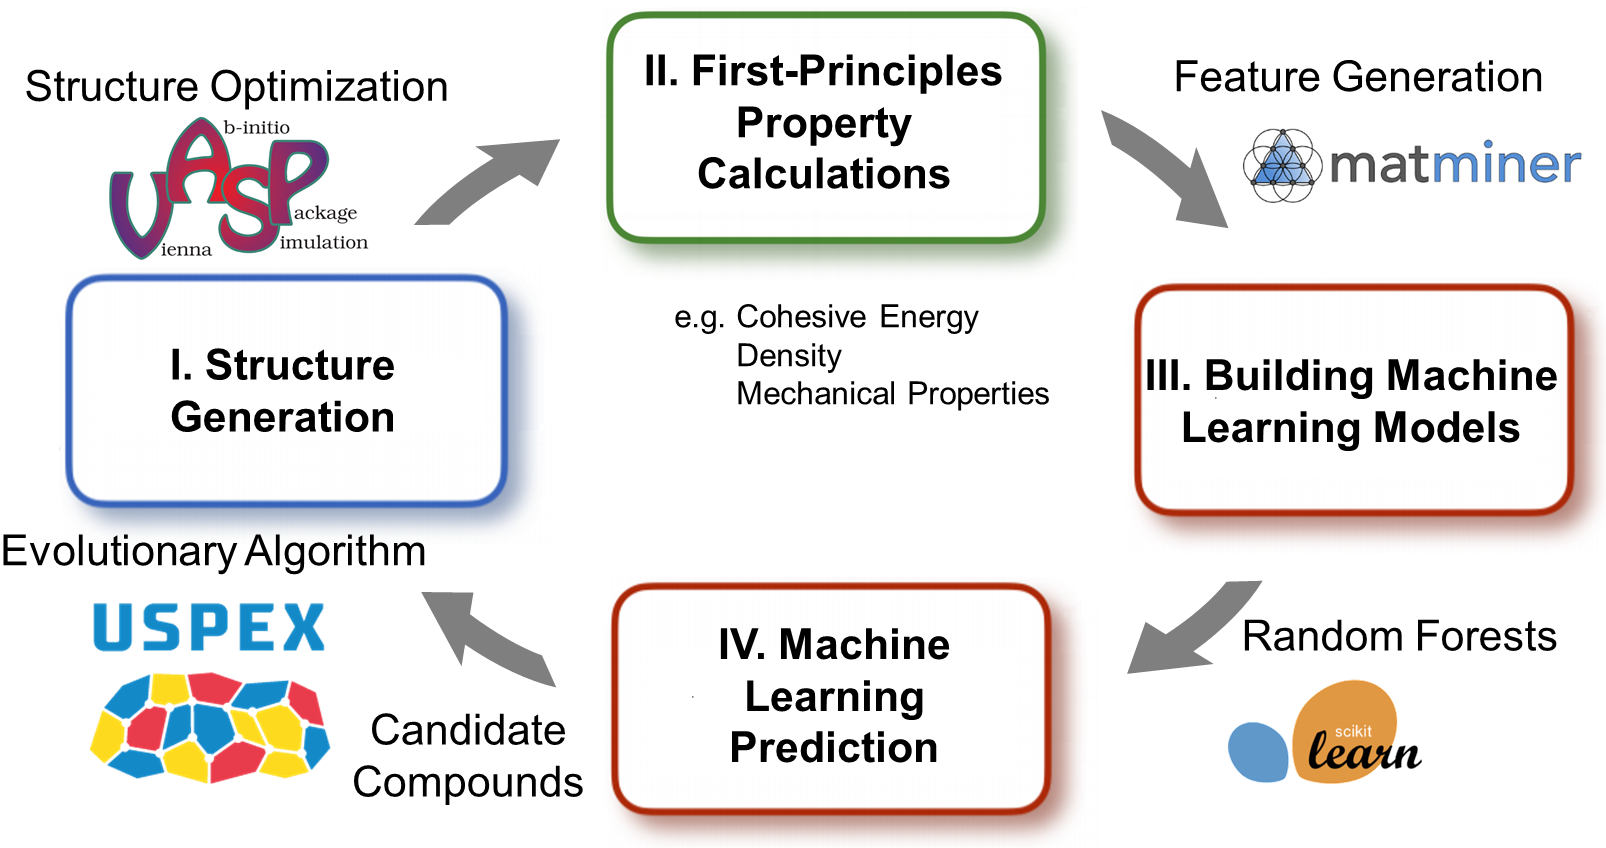
\includegraphics[width=1.0\textwidth]{BNO_1_flowchart.png}
        \caption[The self-improvement recursive procedure used in our B-N-O study.]{The self-improvement recursive procedure used in our B-N-O study. This procedure helps us
        gradually improve our ML models and locate atomic compositions of superhard B-N-O compounds. {\bf I.} Structure generation as data generation for machine learning. {\bf II.} First-principles property calculations as targets including cohesive energy, density, and mechanical propertie. {\bf III.} Building random forests models based on the features generated by \textsc{matminer} library. {\bf III.} Machine learning prediction by mapping out the properties in triangular plots. The promising B-N-O materials are then selected in next round of structure generation.}
        \label{fig:BNO_flowchart}
    \end{figure}
    \pagebreak
    

    We first introduce the new study procedure for B-N-O compounds. The new flowchart is shown in Fig. \ref{fig:BNO_flowchart}.
	To achieve high-accuracy ML prediction for exploring B-N-O materials, we first generate B-N-O data through evolutionary crystal structure prediction using DFT enthalpy as the fitness. Here we adopt a recursive process shown in Fig. \ref{fig:BNO_flowchart}. to gradually improve our ML models and to locate atomic compositions of superhard B-N-O compounds. This process involves four steps: (i) Structure generation, (ii) First-principles property calculation, (iii) Building ML models, and (iv) ML prediction. First, we use evolutionary algorithm for CSP to create the first generation B-N-O data. In the evolutionary searches, we conducted two separate evolutionary searches for each chemical formula, and the optimized structures at the end of each search become a data point.
	Next, we use DFT to calculate physical properties including cohesive energy, density, and elastic tensor. With the elastic tensor, we can calculate the bulk modulus and shear modulus, and also Vickers hardness. Besides, we can also evaluate the elastic stability by examining whether the elastic tensor is positive-definite. 
	
	We build ML models for the cohesive energy, density and Vickers hardness. Afterwards, we carry out ML prediction by mapping out the aforementioned properties in triangular plots. The cohesive energy is related to the formation energy if using isolated atoms' total energies as reference points. Therefore, we use cohesive energy to evaluate the thermodynamic stability. Based on the ML prediction of the cohesive energy and hardness, we select promising compounds with high thermodynamic stability and high hardness to be the candidates of next generation data. In this study, we use four data generations to explore superhard B-N-O compounds. In the following, we elaborate the computational details of CSP, DFT calculations, and ML.
	
	{\it Crystal structure prediction as Data Acquisition}  --
	We generate our B-N-O data through CSP using DFT enthalpy as the fitness. The purpose of CSP is to find the stable or metastable structures of a compound knowing only the chemical formula~\cite{wang2014perspective,graser2018machine, oganov2019structure}. In our B-N-O study, we use evolutionary algorithm implemented in USPEX package~\cite{oganov2006crystal, glass2006uspex, lyakhov2013new}, and the new structures are generated by heredity (50\%), mutation (20\%), and random (10\%) operators. During the data generation for ternary B-N-O compounds, the number of atoms in an unit-cell is between 9 to 19 atoms. During our search, we only consider Since our study focuses on superhard compounds, an external pressure $P$ = 15 GPa is added to avoid graphite-like, layered structures. For each atomic composition, we carry out two separate \textsc{uspex} searches, and more than 1200 structures are explored for each. Upon completion, the optimized structures of both \textsc{uspex} searches are further relaxed without external pressure. In the end, we have two data points for a single chemical formula.
	
	{\it Density functional theory} (DFT) {\it calculations} --
	Our DFT calculations are performed by VASP software~\cite{kresse1996efficiency,kresse1996efficient}, which adopts the pseudopotential method and plane-wave basis sets. We use the projector augmented wave (PAW)~\cite{PAW_1,PAW_2} method and generalized gradient approximation (GGA) exchange-correlation energy functional based on Perdew-Burke-Ernzerhof (PBE)~\cite{PBE} formalism. The kinetic energy cutoff for wavefunction expansion is 520 eV, and k-points are sampled by a $\Gamma$-centered Monkhorst-Pack mesh with a resolution $\sim$ 0.02 $\times$ 2$\pi$/\text{\normalfont\AA}. The convergence criteria of electronic self-consistency and structural relaxation are set to 10$^{-6}$
	eV/unit cell and 10$^{-3}$ eV/$\text{\normalfont\AA}$, respectively. 
	
	The strain-stress method~\cite{PhysRevB.65.104104} implemented in VASP is used to compute the elastic constants $C_{ij}$, which in turn allows us to evaluate the elastic stability and mechanical properties. In our calculations, we carried out properties including eigenvalues of elastic tensor, Voigt-Reuss-Hill (VRH) average~\cite{voigt1928lehrbuch, reuss1929berechnung, hill1952elastic} for bulk/shear modulus, and Vickers hardness by Chen's model~\cite{chen2011modeling} directly through MechElastic python library~\cite{singh2018elastic, singh2021mechelastic}. Phonon density of states are computed using the \textsc{Phonopy} package~\cite{phonopy} through density functional perturbation theory (DFPT) scheme implemented in VASP, and all of the convergence tests are examined carefully.


	
	
	{\it Machine Learning models and prediction --} 
	After the preparation of ML data, we build our ML models for cohesive energy, density, and hardness. Since the quality of ML data determines the predictive capability, we first exclude elastically unstable structures in the data set by examining whether the elastic tensor is positive-definite. Next, we create features or descriptors to train our ML model using \textsc{Matminer}~\cite{matminer} python library. For the prediction of cohesive energy, we adopt the composition features proposed by Meredig $et$ $al.$~\cite{meredig2014combinatorial}. In our B-N-O study, a total number of 16 features are considered: fraction of B/N/O, mean of atomic weight, mean column, mean row, range of atomic number, mean of atomic number, range of atomic radius, mean of atomic radius, range of electronegativity, mean of electronegativity, average of s/p electron, fraction of s/p electron. For the hardness model, we add one extra structural property, density, to improve the model performance. As a result, we also build the density model using 16 compositional features to evaluate the density for hardness prediction. The adopted ML algorithm in our study is random forests, which is implemented in \textsc{scikit-learn} python library~\cite{scikit-learn}. 
    
	
	\begin{figure}[htbp]
        \centering
        \captionsetup{singlelinecheck = false, justification=justified}
        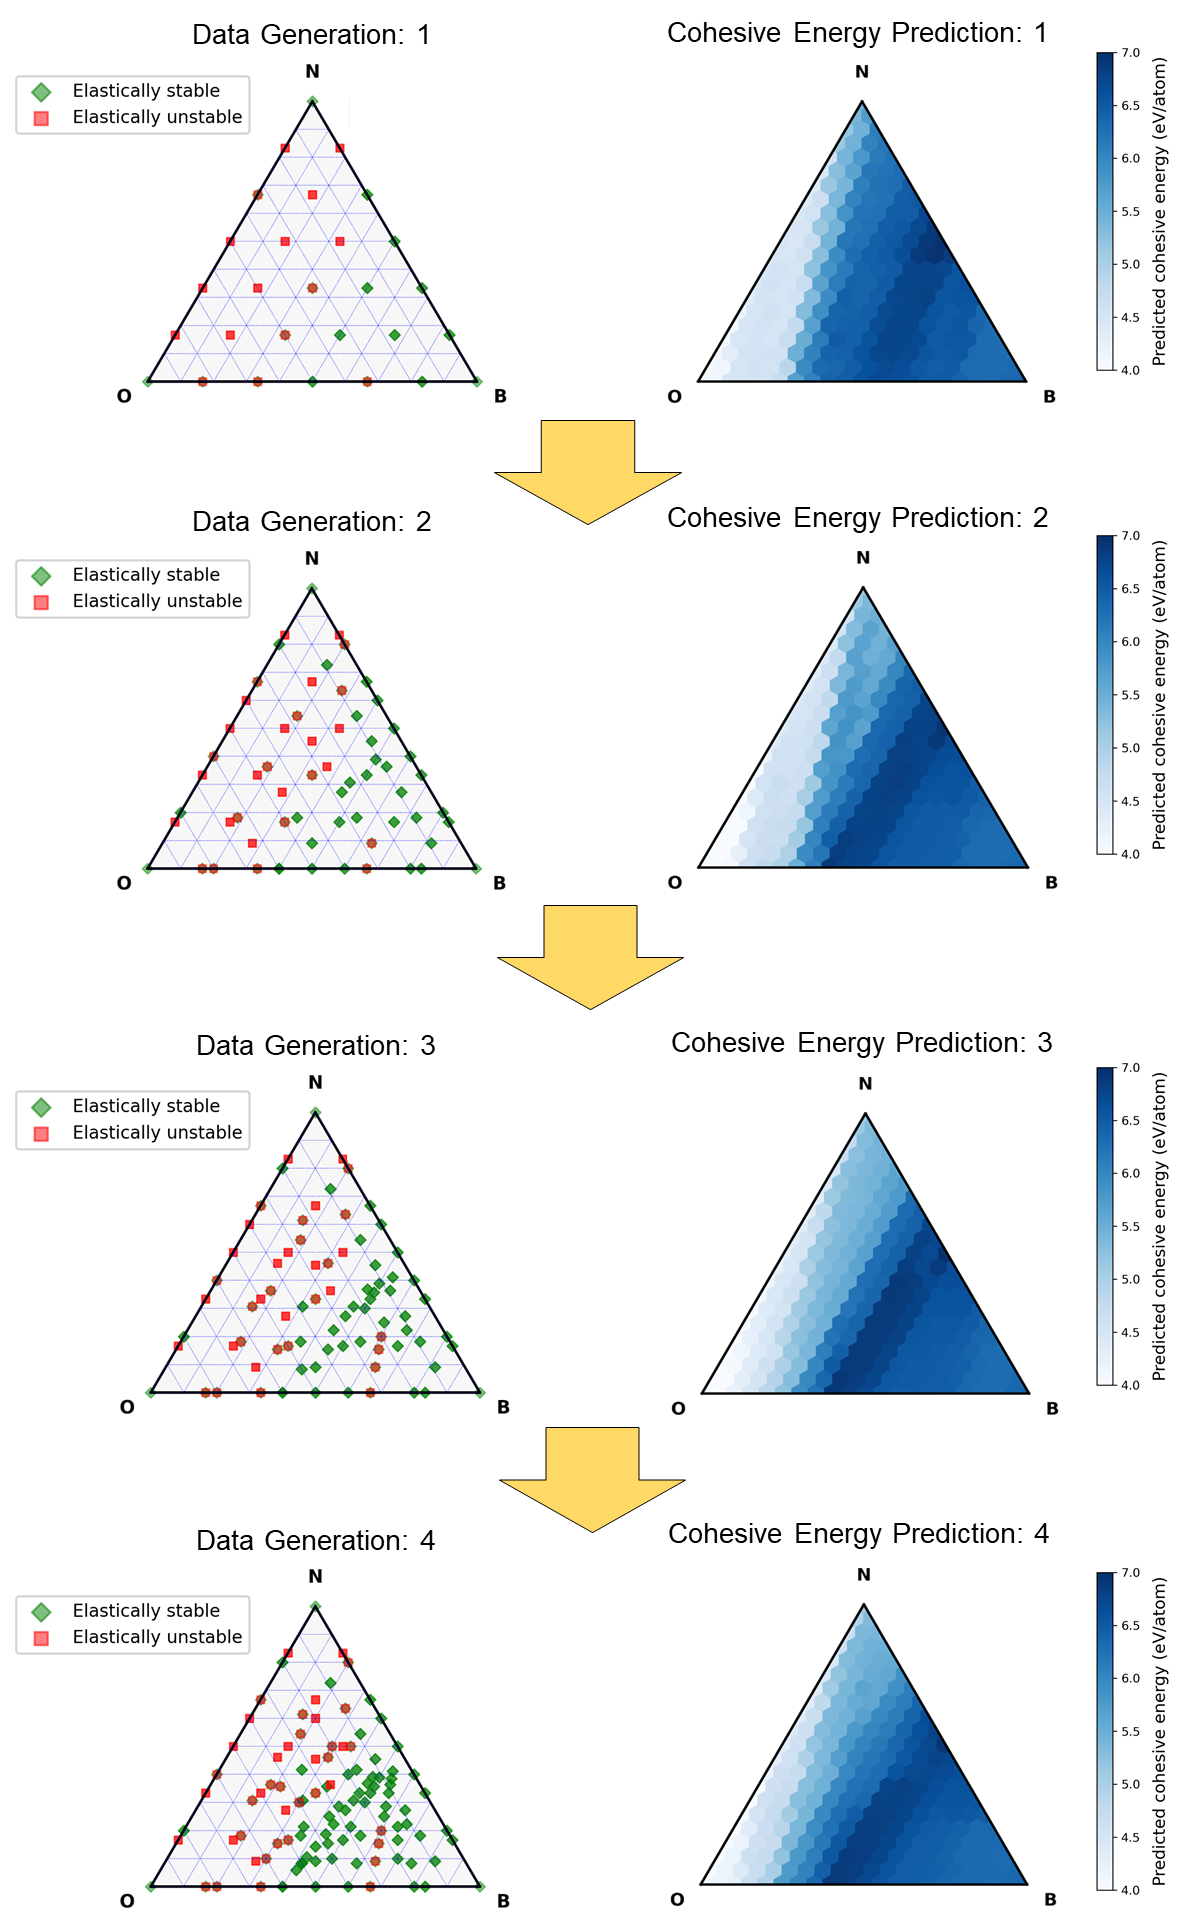
\includegraphics[width=0.8\textwidth]{BNO_2_data.png}
        \caption[Data distribution and predicted cohesive energy in composition space of B-N-O systems]{Data distribution (top) and predicted cohesive energy (bottom) in composition space of B-N-O systems. In the top row, the green diamond and red rectangle represent the elastically stable and unstable structures from evolutionary algorithm searches.}
        \label{BNO_2_data}
    \end{figure}
    \pagebreak

    In Fig. \ref{BNO_2_data}, we show the evolution of our machine data generated by \textsc{uspex} package and the corresponding random forests models for cohesive energy. In the beginning, we have an uniform sampling with a number of atoms equal to 12 for binary and ternary compounds. (The elemental B, N and O are based on the known structures.) For example, pure B here is a $\alpha$-B$_{12}$. In the first generation sampling, we have found the rate between elastically stable and unstable structures is roughtly 1:1. Although the grid is course, we can see that if a ternary compound is composed of mostly nitrogen and oxygen atoms, they tend to be elastically unstable. On the other hand, if the boron content is high, then such systems are more likely to be elastically stable. To ensure high accuracy of ML prediction, we only consider elastically stable structures to build our ML models. In these four generations, the numbers of (elastically stable) data involved in building ML models are 27, 78, 104, and 153, respectively.
    
    From cohesive energy prediction of first generation, we notice that when the boron content is large, the cohesive energy is also high, indicating higher thermodynamic stability. Therefore, the behavior of elastic stability and thermodynamic stability are consistent with each other. Besides, based on the such predicting results, starting from data generation 2, we neglect the composition with simultaneous high nitrogen and high oxygen contents. In the subsequent generations, we manually select more compositions based on the ML prediction of previous generation. In particular, we gradually increase the compositions with high predicted cohesive energy and predicted hardness. We find that the machine learning prediction results have higher and higher resolution during this process. Importantly, we found that in cohesive energy prediction, a region connecting BN and B$_2$O$_3$ have high cohesive energy. This result is consistent with the recently synthesized B$_6$N$_4$O$_3$ by Bhat {\it et al.}, where a mixture of hexagonal BN and B$_2$O$_3$ is used as starting materials for HPHT treatment.

	\begin{figure}[htbp]
        \centering
        \captionsetup{singlelinecheck = false, justification=justified}
        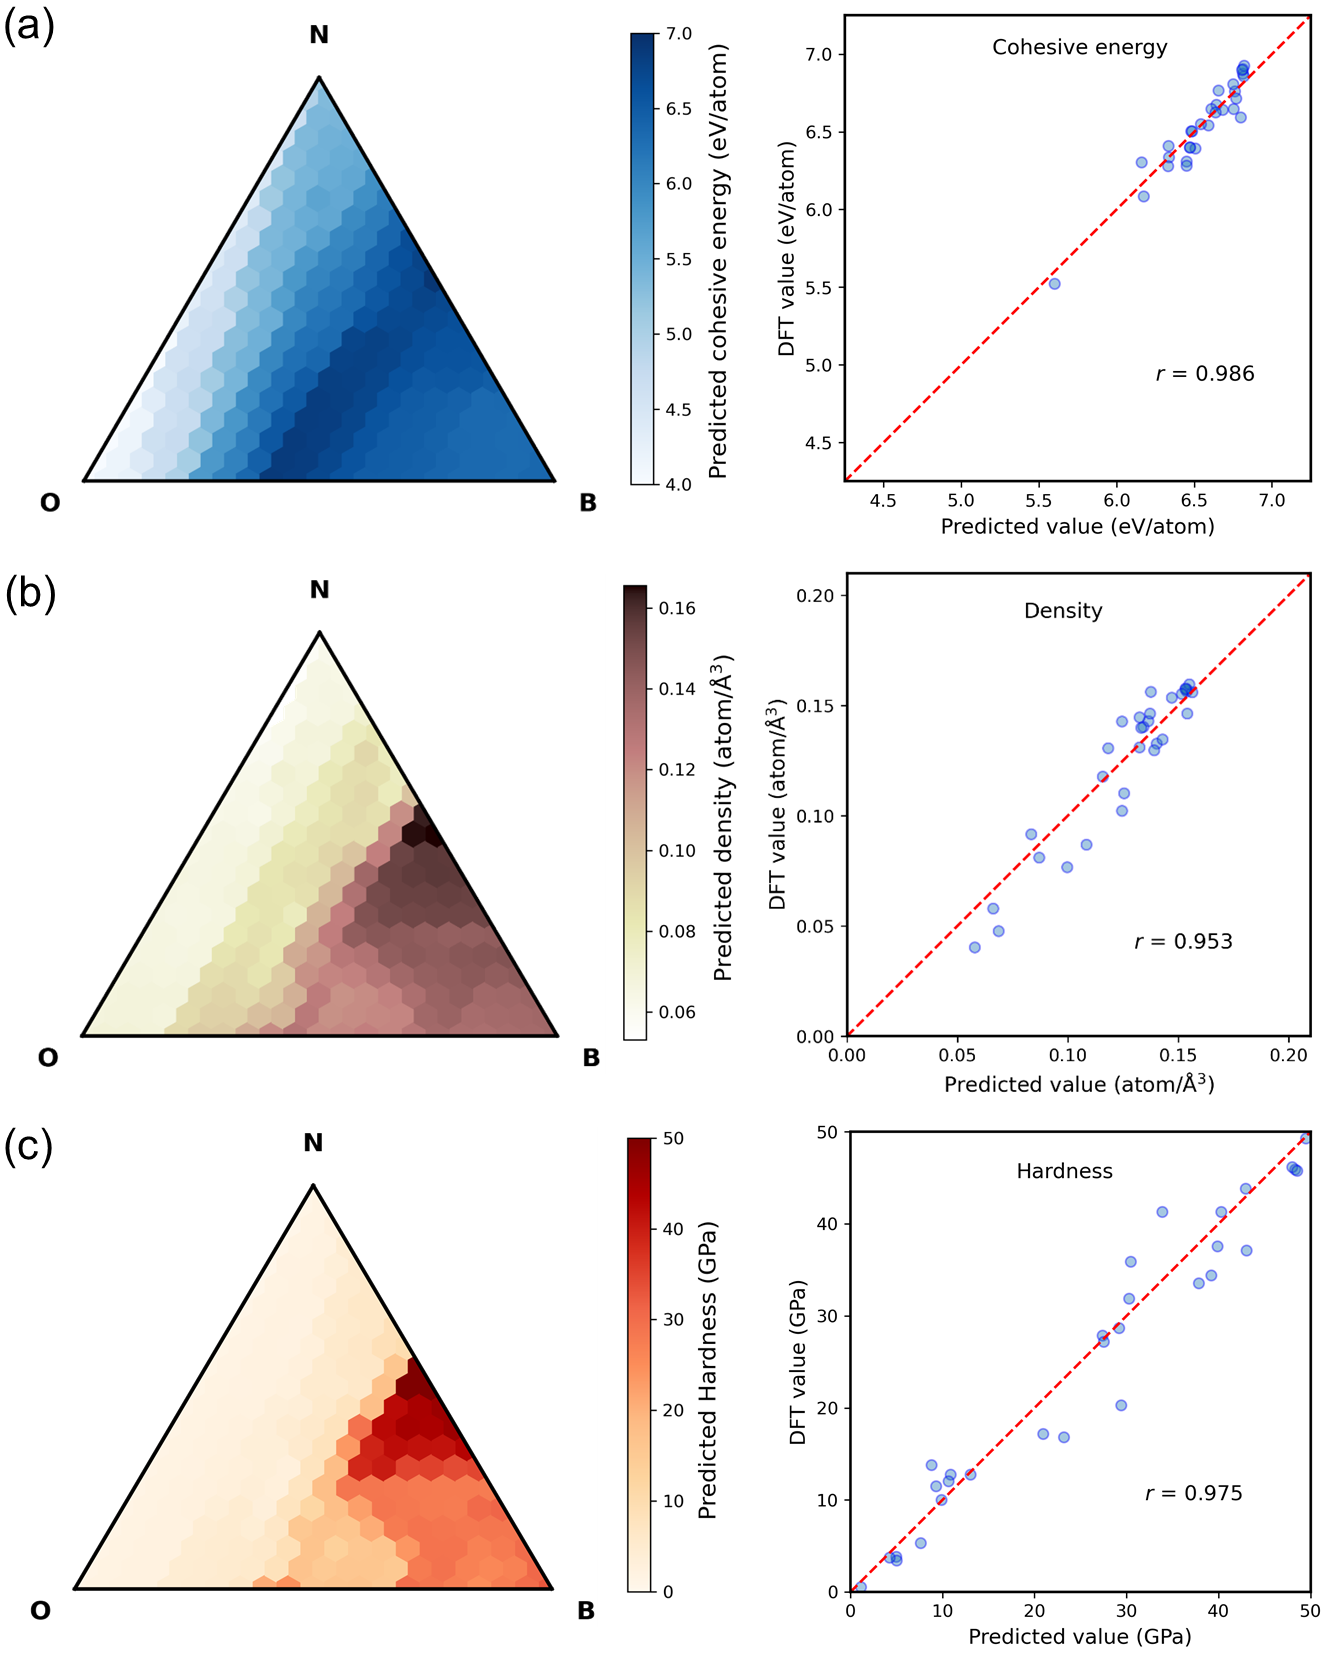
\includegraphics[width=0.85\textwidth]{BNO_3_model.png}
        \caption[Machine learning prediction of cohesive energy, density, and hardness as well as corresponding model evaluations.]{Machine learning prediction of (a) cohesive energy, (b) volumetric density, and (c) hardness using the data of generation 4 (left column) and corresponding model evaluation using test set (20 \% of data) (right column).}
        \label{fig:BNO_3_model}
    \end{figure}
    \pagebreak

    Fig. \ref{fig:BNO_3_model} shows the predicting results of our random forests models for cohesive energy, density, and hardness built from data generation 4. Here, 80 \% of data are used to construct random forests models (for training and validation), and the remaining 20 \% of data are used for final evaluation. Our cohesive energy model shows a Pearson correlation coefficient $r = 0.98$, which demonstrates the accuracy of the model. 

    Based on our previous ML study for B-C-N compounds, we have noticed that the hardness value has a positive correlation with volumetric density. Therefore, here we also consider density as a feature to build our hardness model. The hardness values here are computed using Chen's model \cite{chen2011modeling}
	\begin{equation}
		\label{eq:Chen}
		\begin{aligned}
			H_V = 2(k^2G)^{0.585}-3,
		\end{aligned}
	\end{equation}
	where $k = G/K$ is pugh's ratio, $G$ is shear modulus, and $K$ is bulk modulus.

	%\begin{table*}[htbp]
	\begin{table*}[t]
		\begin{center}
		\caption[Mechanical properties of newly-found superhard B-N-O compounds]{Mechanical properties of superhard B-N-O compounds with cohesive energy $>$ 6.75 eV discovered in this study. Density $\rho$ (atom/$\text{\normalfont\AA}^3$), bulk modulus $K$ (GPa), shear modulus $G$ (GPa), cohesive energy $E_{coh}$ (eV/atom), and formation energy $E_{form}$ (meV/atom).}
		\label{tab:BNO}
		\begin{tabular}{l|c|c|c|c|c|c} % <-- Alignments: 1st column left, 2nd middle and 3rd right, with vertical lines in between
			Crystal   & $\rho$ & $K$ & $G$ & $H$ & $ E_{coh}$ & $E_{form}$ \\
			%     $\alpha$ & $\beta$ & $\gamma$ \\
			\hline
			B$_5$N$_3$O$_2$      & 0.151 & 286  & 257  & 42 & 6.761 & \\
			B$_5$N$_3$O$_3$ (WZ) & 0.150 & 279  & 255  & 43 & 6.935 & 83 \\
			B$_6$N$_4$O$_2$      & 0.156 & 322  & 284  & 44 & 6.810 & \\
			B$_6$N$_4$O$_3$ (ZB) & 0.155 & 292  & 268  & 45 & 6.900 & 120 \\
			B$_7$N$_5$O$_2$      & 0.146 & 272  & 241  & 40 & 6.776 & \\
			B$_7$N$_5$O$_3$ (ZB) & 0.158 & 306  & 283  & 47 & 6.904 & 117 \\
			B$_9$N$_7$O$_2$      & 0.161 & 330  & 296  & 46 & 6.802 & \\
			B$_9$N$_7$O$_3$ (ZB) & 0.160 & 318  & 301  & 50 & 6.926 & 97 \\
			cubic BN             & 0.168 & 373  & 383  & 64 & 7.028 & 0 \\
			B$_2$O$_3$ (P3$_1$21)& 0.101 &   35 & 33   & 12 & 7.008 & 0
		\end{tabular}
		\end{center}
	\end{table*}    



    In order to map out the hardness values of ternary B-N-O compounds, we first build a density model based on compositional features. The built density model is used to predict density, which in turn becomes the density feature for hardness prediction. As shown in Fig. \ref{fig:BNO_3_model}, the predicted density and hardness show a highly positive correlation with each other. The results show that ternary B-N-O compounds can have superhardness around a region near binary BN, which has a predicted hardness like cubic boron nitride. Following our study procedure shown in Fig. \ref{fig:BNO_flowchart}, now we can find the superhard B-N-O compounds directly by inspecting the data generated from evolutionary algorithm. The predicted ternary B-N-O compounds with superhardness are listed in Table \ref{tab:BNO}. We found that the compositions of discovered superhard B-N-O compounds have two kinds. For the first kind, the number of boron is equal to the sum of nitrogen and oxygen (e.g. B$_5$N$_3$O$_2$). The second kinds has one more oxygen, so the number of boron is equal to the sum of nitrogen and oxygen plus 1 (e.g. B$_5$N$_3$O$_3$). First, by examining the density of states, these materials are insulators with wide bandgaps greater than 4.5 eV based on modified Becke Johnson (mBJ) potentail \cite{mBJ_1,mBJ_2}. To evaluate their thermodynamic stability, we can compare their cohesive energy,
    \begin{equation}
	\label{eq:cohesive}
	\begin{aligned}
		E_{coh} =  \frac{xE(B_{atom}) + yE(N_{atom}) + zE(O_{atom}) - E(B_xN_yO_z)} {x+y+z},
	\end{aligned}
	\end{equation}
    
    which can be regarded as the formation energy with a minus sign using the total energies of isolated atoms as references. Therefore, higher cohesive energy means higher thermodynamic stablity of a material. We found that the second kind have a higher cohesive energy than the first kind. Besides, we also find that the cohesive energies of c-BN and B$_2$O$_3$ are higher than discovered B-N-O compounds. This result implies that the discovered B-N-O compounds are metastable at ambient pressure condition. Besides, the chemical formula of the second kind has a form: B$_{x+2}$N$_x$O$_{3}$, and this allows us to calculate the formation energy using the total energies of c-BN and B$_2$O$_3$ as references. Hence, the formation energy for the second kind can be computed by
	\begin{equation}
	\label{eq:formation}
	\begin{aligned}
		E_{form} =  \frac{E(B_{x+2}N_xO_{3}) - xE(c-BN) - E(B_2O_3) } {2x+5}.
	\end{aligned}
	\end{equation}
    We found that B$_5$N$_3$O$_3$ has the lowest formation energy in our study, and this property might be related to its superlattice structure shown in Fig. \ref{BNO_4_DFT}(a). Besides, the report from Bhat {\it et al.} also found their ordered structure models are in better agreement with experiment experiment. As a result, the superlattice structure might exist in B-N-O compounds.
    
    Next, we conduct more theoretical characterization for the more stable B-N-O compounds with their chemical formulae as B$_{x+2}$N$_x$O$_{3}$.
    In Fig. \ref{BNO_4_DFT}, we show crystal structure, electronic density of states (DOS), and phonon DOS for B$_5$N$_3$O$_3$, B$_6$N$_4$O$_3$, B$_7$N$_5$O$_3$, and B$_9$N$_7$O$_3$. From their crystal structure, only B$_5$N$_3$O$_3$ has a wurtzite-type structure, and the other three compounds have zinc-blende-type structure. We note that if comparing these chemical formulae with BN, we can find that the one boron atom is missing (due to B$_2$O$_3$), and this is associated with vacant boron sites in these materials. The vacant boron sites are shown in Fig. \ref{BNO_5_vacancy}. By calculating the phonon DOS (shown in the right column of Fig. \ref{BNO_4_DFT}), our results ensure the dynamical stability in these B-N-O compounds.
    
    We also calculate the electronic DOS of these four structures. We find that the three zinc-blende type structures have similar electronic DOS around Fermi level. The DOS of wurtzite-type B$_5$N$_3$O$_3$ is also similar, but it shows a very wide bandgap roughly 2 eV greater than zinc-blende type B-N-O compounds. This result is unusual because in binary BN structures, wutzite BN has a smaller bandgap than cubic BN, which is completely different from the ternary B-N-O compounds.

	\begin{figure}[htbp]
        \centering
        \captionsetup{singlelinecheck = false, justification=justified}
        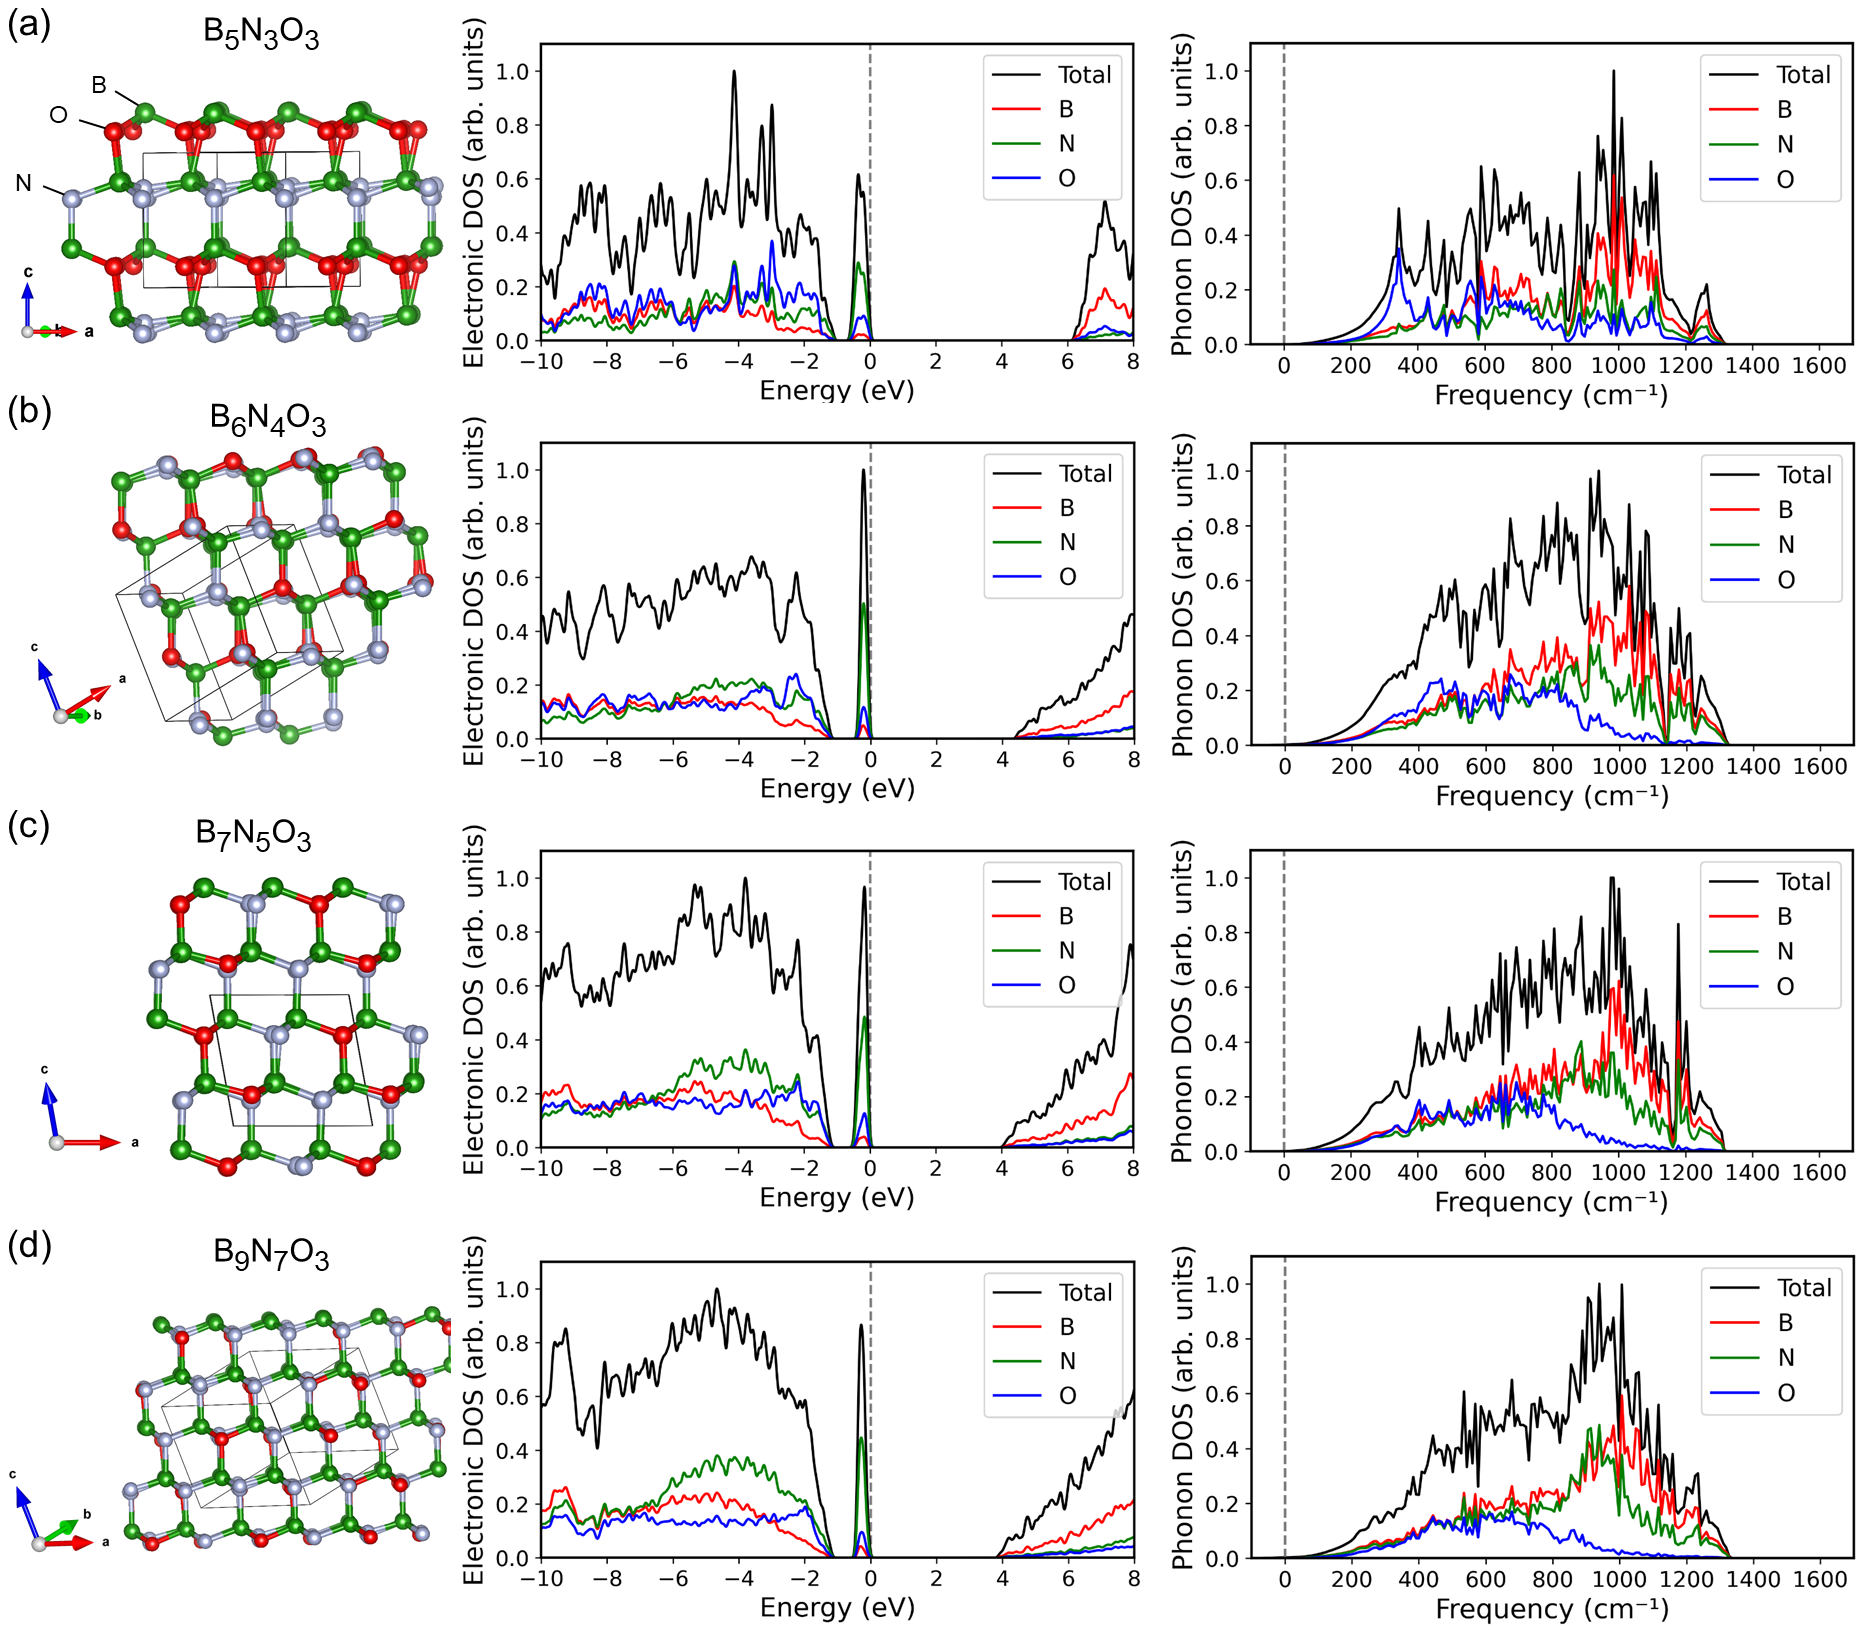
\includegraphics[width=1.0\textwidth]{BNO_4_DFT.png}
        \caption[Crystal structures, electronic density of states, and phonon density of states of superhard B-N-O compounds.]{Crystal structure [left column], electronic density of states [middle column], and phonon density of states of superhard (a) B$_5$N$_3$O$_3$, (b) B$_6$N$_4$O$_3$, (c) B$_7$N$_5$O$_3$, and (d) B$_9$N$_7$O$_3$ discovered by evolutionary crystal structure prediction. }
        \label{BNO_4_DFT}
    \end{figure}
    \pagebreak
    
    A remarkable thing to be mentioned here is that all of the density of states show a sharp peak at valence band maximum. This peak is contributed from the localized states of nitrogen atoms being adjacent to the vacant boron sites. The charge distribution of the peak in the DOS of B$_5$N$_3$O$_3$ is shown by the contour in  Fig. \ref{BNO_5_vacancy}. Besides, we find that in zinc-blende-type structures, the bandgap increase with increasing oxygen content. This result is reasonable because B$_2$O$_3$ has an extremely large band gap greater than 10 eV \cite{B2O3_10eV} comparing with the bandgap of 6 eV for c-BN. Overall, by introducing oxygen atoms in binary BN compounds, the electronic structures can be modified substantially, which might also lead to changes in the thermal and chemical stabilities.
    
	\begin{figure}[htbp]
        \centering
        \captionsetup{singlelinecheck = false, justification=justified}
        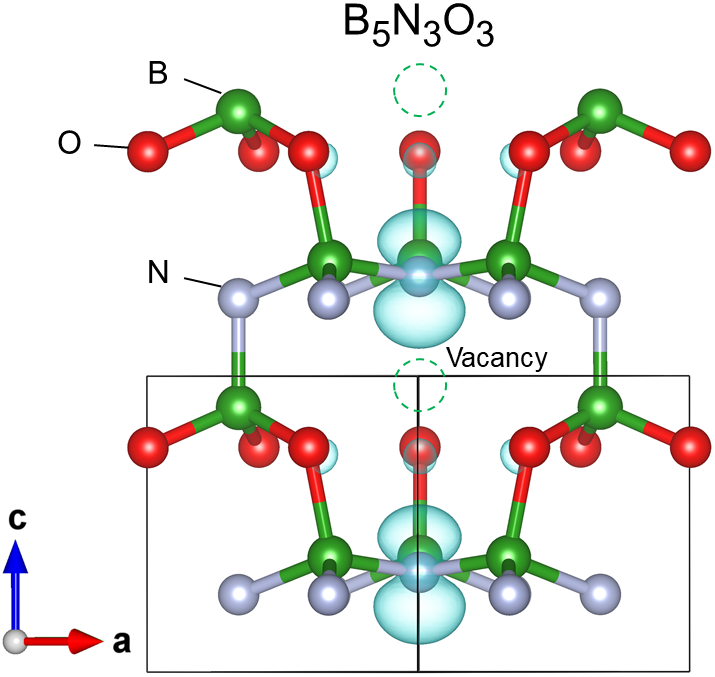
\includegraphics[width=0.6\textwidth]{BNO_5_vacancy.png}
        \caption[Crystal structure of B$_5$N$_3$O$_3$ highlighting the vacancies and electron density distribution of the valence band maximum states]{Crystal structure of B$_5$N$_3$O$_3$ highlighting the vacancies near three oxygen atoms and one nitrogen atom. The contour represents the electron density distribution of the electronic states at valence band maximum.}
        \label{BNO_5_vacancy}
    \end{figure}
    \pagebreak

    In summary, we have used a recursive study procedure to search for superhard B-N-O compounds using machine learning techniques, where we generated the data based on the evolutionary searches and density functional theory. Our results show that thermodynamically stable and superhard B-N-O materials have a chemical formula B$_{x+2}$N$_{x}$O$_3$ (x $\ge$ 3), and their hardness values are around 45 GPa. Besides, that are all have very large bandgap $>$ 4 eV based on PBE functional. Since the DFT-PBE results tend to underestimate bandgaps, the actual values of bandgaps should be even larger. Their electronic density of states all have a prominent peak around valence band maximum (VBM), which is corresponding to a localized state at nitrogen atoms around the vacant sites. Due to the change of electronic structure, the newly-found B-N-O materials might have a better performance than cubic BN in the humid condition at high temperature. 


    
    \pagebreak

    
    %\chapter{4 STRUCTURAL AND TOPOLOGICAL PHASE TRANSITIONS IN TOPOLOGICAL QUANTUM MATERIALS}
    \addtocounter{numch}{1}
	\addcontentsline{toc}{chapter}{\hspace{0pt}  \the\value{numch} \hspace{-4pt} STRUCTURAL AND TOPOLOGICAL PHASE TRANSITIONS IN \linebreak \hspace*{6pt} TOPOLOGICAL QUANTUM MATERIALS}
	{\centering
		\vspace{0pt} \hspace{0pt} \par
	}
	{\centering
		\vspace{56pt} CHAPTER  \the\value{numch}
	}
	{\centering\singlespacing
		STRUCTURAL AND TOPOLOGICAL PHASE TRANSITIONS IN TOPOLOGICAL QUANTUM MATERIALS
	    \par
	}
	{\centering
		\vspace{0pt} \hspace{0pt} \par
	}
	

    
    %\subsection*{Topological Phase Transition in ZrTe$_5$}
    \addcontentsline{toc}{subsection}{Topological Phase Transition in ZrTe$_5$}
	{\centering
		\vspace{12pt} Topological Phase Transition in ZrTe$_5$
	    \par
	}
Topological materials with symmetry-protected boundary modes has fundamentally opened a entire new filed in condensed matter physics. Three dimensional band insulators with time-reversal (TR) symmetry can be classified into three kinds: normal insulators (NIs), weak topological insulators (WTIs), and strong topological insulators (STIs). Such classification is based on four topological $Z_2$  invariants or $Z_2$ indices. Here, our goal is to study topological phase transition by manipulating the band structure, which requires closing and reopening the bandgap. In order to achieve band inversion, it is easier to choose a material with small gap between valence and conduction bands. Zirconium pentatellurides ZrTe$_5$ has a mall direct band gap at $\Gamma$ point, and hence is an ideal material to study topological phase transition.

	\begin{figure}[htbp]
        \centering
        \captionsetup{singlelinecheck = false, justification=justified}
        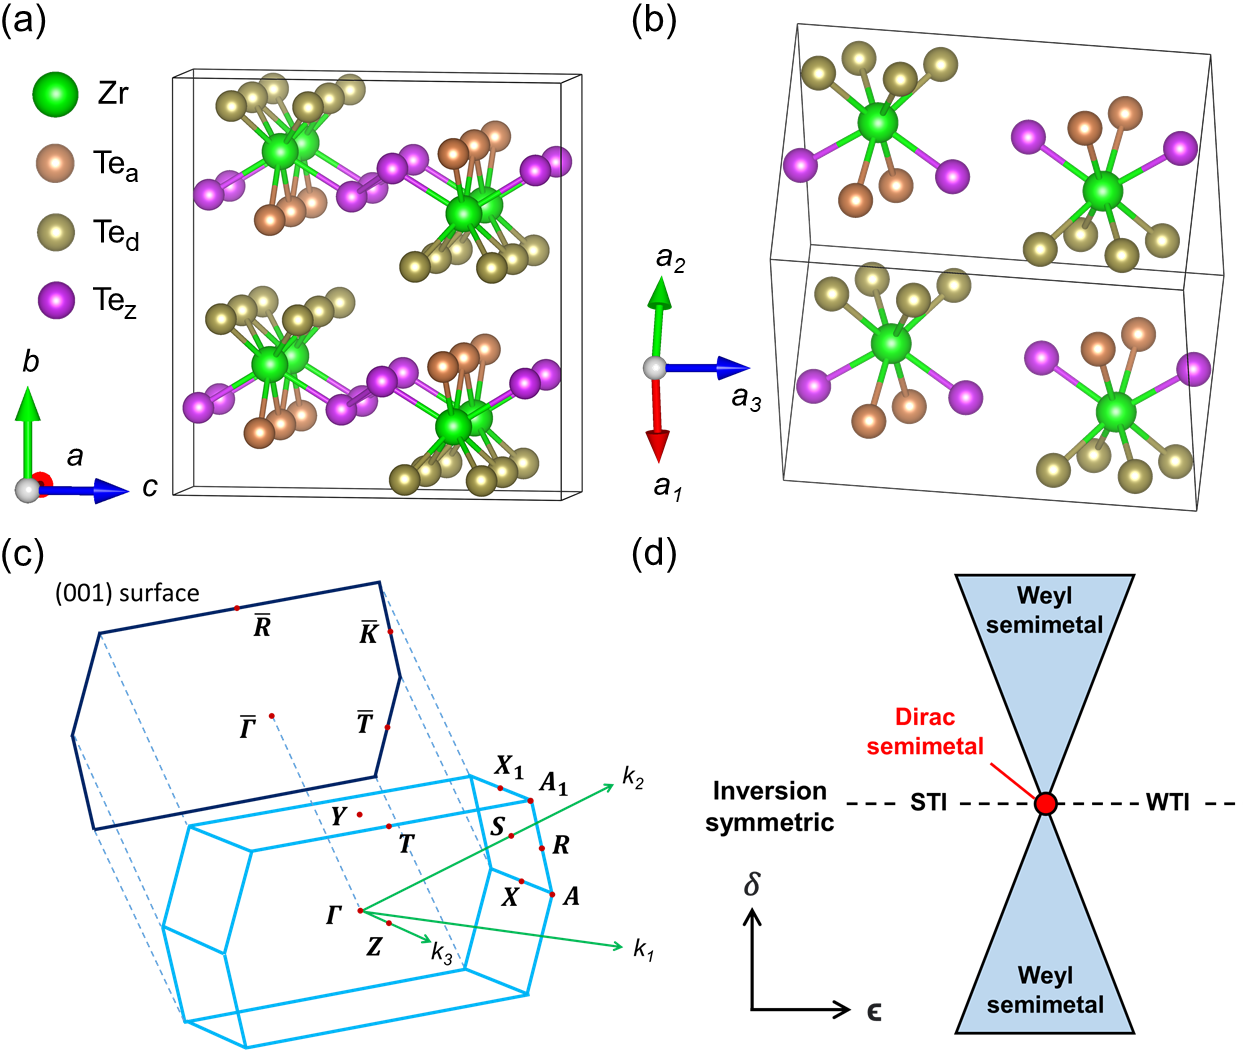
\includegraphics[width=1.0\textwidth]{ZrTe5_structure.png}
        \caption[Crystal structure and Brillouin zone of ZrTe$_5$ as well as the universal phase diagram of topological insulators.]{Crystal structure of ZrTe$_5$ in (a) conventional cell, and (b) primitive cell. (c) Bulk and surface Brillouin zones of ZrTe$_5$. (d) Universal phase diagram of topological insulators proposed by Murakami for a 3D system \cite{murakami2008universal, murakami2007phase}. The control parameter $\delta$ describes the breaking of inversion symmetry. The control parameter $\epsilon$ does not break inversion symmetry.}
        \label{ZrTe5_structure}
    \end{figure}
    
ZrTe$_5$ is a van der Waals (vdW) layered material crystallized in the $Cmcm$ orthorhombic space group as shown in Fig. \ref{ZrTe5_structure}(a). Each layer consists of ZrTe$_3$ (1 Te$_a$ and 2 Te$_d$) chains extending along the {\it x} direction, and the layers are stacked along the {\it y} direction. The material has received substantial interest because its monolayer form is predicted to be a large bandgap quantum spin Hall insulator \cite{weng2014transition}. It was also suggested that the 3D bulk band structure is very close to the phase boundary between WTI and STI.

Early studies of optical conductivity \cite{chen2015optical}, quantum oscillations \cite{liu2016zeeman, nair2018thermodynamic}, photoemission, and negative longitudinal magnetoresistance
(NLMR) \cite{li2016chiral} have supported the predicted Dirac semimetal-like band structure in the bulk, with a single Dirac point at the center of the Brillouin zone. Unlike topological Dirac semimetals such as Na$_3$Bi or Cd$_3$As$_2$, there is no additional crystalline symmetry to protect the Dirac point in ZrTe$_5$, and more recent spectroscopy measurements revealed that its band structure is better described by a massive Dirac dispersion, where mass plays the role of bandgap. The bandgap size measured by different experiments varies, ranging from 10 to 80 meV, and there are conflicting reports on whether the material is a WTI or STI \cite{li2016experimental, chen2017spectroscopic, jiang2017landau, xiong2017three}, or changes with temperature \cite{xu2018temperature}. These experimental findings suggest that the electronic structure of ZrTe$_5$ may be very sensitive to external perturbation, such as lattice distortion.

The relationship between these phases is summarized in the general phase diagram proposed by Murakami and Kuga \cite{murakami2008universal, murakami2007phase}, as shown in Fig. \ref{ZrTe5_structure} (d). These topological phases have been intensively studied in the past decade. In contrast, the transition between these phases is less explored because it requires changing the band parameters of the solid. It has been demonstrated that topological phase transitions can be induced either by chemical doping or by thermal lattice expansion \cite{xu2011topological, wu2013sudden, dziawa2012topological, xu2012observation}. Nevertheless, the precise $in$ $situ$ control of topological phase transition in a three-dimensional (3D) system is still challenging. 


{\it Methods --}The electronic structure and energy gap of ZrTe$_5$ under strain were calculated by the Quantum Espresso package \cite{giannozzi2009quantum} based on DFT. The Perdew-Burke-Ernzerhof exchange-correlation functional (PBE-GGA) \cite{PBE} with spin-orbit coupling and projector augmented wave \cite{PAW_1} method were used. The unstrained lattice parameters (a = 3.97976 Å, c = 13.6762 Å) were determined by experimental data at 10 K \cite{fjellvaag1986structural}, and an 11 $\times$ 11 grid in the parameter ranges of 1.0$a$ to 1.02$a$ and 0.99$c$ to 1.01$c$ was considered for studying the gap behavior with lattice variation. An 8 $\times$ 8 $\times$ 4 momentum grid was used in the self-consistent calculation, and the kinetic energy cutoff and convergence criterion were set to 30 and 10$^{-7}$ rydberg, respectively.

The topological Z$_2$ indices of different strained structures were also computed to identify their topological nature. With input from the electronic structure calculations of Quantum Espresso, the maximally localized Wannier functions were first computed using the Wannier90 package \cite{wannier90}, which, in turn, allowed the determination of Z$_2$ indices by tracking hybrid Wannier charge centers using the WannierTools package \cite{wanniertools}. In this study, phase transition between the STI and WTI states was directly controlled by closing the energy gap at the Brillouin zone center.

Additional structure relaxation calculations were performed with the vdW-DFT \cite{thonhauser2007van,berland2015van}, corrected using the exchange-hole dipole moment model \cite{otero2012van}. The vdW-DFT fully relaxed lattice parameters of layer-structured ZrTe$_5$ are within 1\% error compared to the unstrained experimental data. To determine the Poisson ratio, conventional cells of different fixed lattice parameters along the a axis were considered, while the b and c lattice parameters were allowed to evolve freely in the structure relaxation calculations.

	\begin{figure}[htbp]
        \centering
        \captionsetup{singlelinecheck = false, justification=justified}
        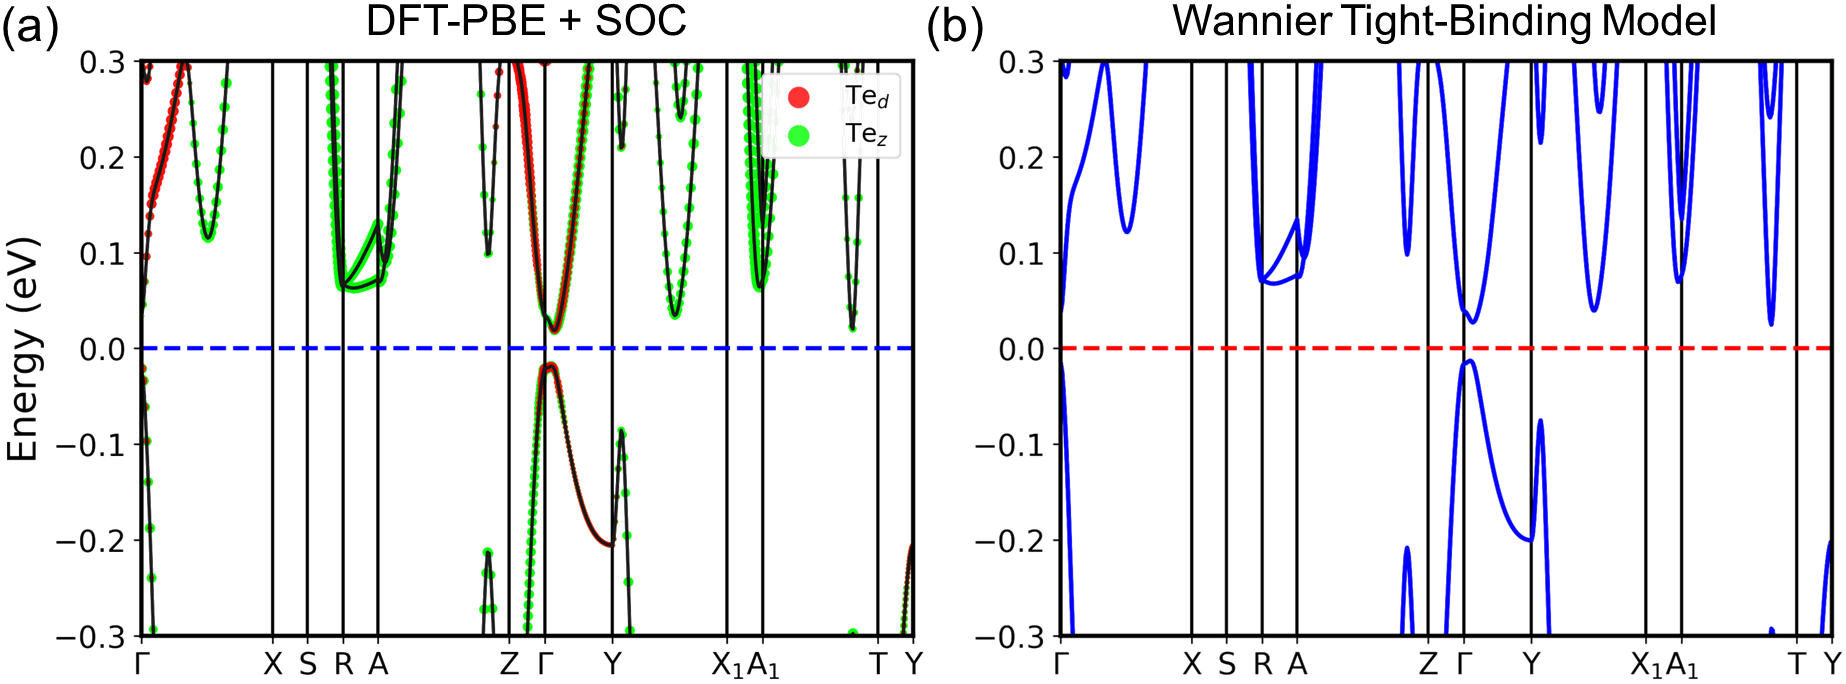
\includegraphics[width=0.95\textwidth]{ZrTe5_bands.png}
        \caption[Band structures calculated by DFT and tight-binding model.]{Band structures calculated by (a) DFT and (b) Wannier tight-binding model from Wannier90 package \cite{wannier90}. The high symmetry points can be found in Fig. \ref{ZrTe5_structure}(c). Here, the Wannier tight-binding model perfectly reproduces the DFT band structure around Fermi level.}
        \label{ZrTe5_bands}
    \end{figure}

In order to identify the $Z_2$ indices of ZrTe$_5$, we first calculate the band structure (with spin-orbit coupling) based on experimental crystal structure \cite{fjellvaag1986structural}, and we next use Wannier90 package \cite{wannier90} to obtain the corresponding tight-binding model. The band structures calculated by DFT and the Wannier tight-binding model are shown in Fig. \ref{ZrTe5_bands}. The band structure based on Wannier tight-binding model is identical to DFT band structure around Fermi level. Therefore, we use the Wannier tight-binding model to compute the topological $Z_2$ indices using WannierTools package \cite{wanniertools}. In WannierTools, it is capable of identifying the $Z_2$ indices by tracking hybrid Wannier charge centers \cite{PhysRevB.83.235401}. In this method, first the hybrid Wannier function is defined as 
	\begin{equation}
		\begin{aligned}
		|nk_xl_y\rangle =\frac{1}{2\pi} \int_0^{2\pi}d k_y e^{-ik_yl_y}|\psi_{n{\bold k}}\rangle,
		\end{aligned}
	\end{equation}
where $|\psi_{n{\bold k}}\rangle$ is the Bloch wave function. The hybrid Wannier charge center (WCC) $\bar{y}_n$ can be defined as a function of $k_x$ by integrating over $k_y$:
	\begin{equation}
		\begin{aligned}
		 \bar{y}_n(k_x)&=  \langle nk_x0|y|n k_x0\rangle \\
            &=\frac{i}{2\pi} \int _{-\pi} ^{\pi}d {k_y} \left \langle u_{n,k_x, k_y} \left| \frac{\partial}{\partial k_y} \right| u_{n,k_x, k_y}\right \rangle,
		\end{aligned}
	\end{equation}
where $| u_{n{\bf k}}\rangle$ is the periodic part of Bloch function $|\psi_{n{\bf k}}\rangle$. One can find more information in Ref. \cite{wanniertools}.

Figure \ref{ZrTe5_wcc} shows the WCC evolution for six time-reversal invariant planes corresponding to the BZ of primitive cell. The strong index can be obtain by checking either (a), (b), or (c). One plane has a $Z_2 = 1$ and the other has a $Z_2 = 0$, so the strong index is 1. For the weak indices, by checking the right column of Fig. \ref{ZrTe5_wcc}, we know ($\nu_1\nu_2\nu_3$) is (110). Therefore, the band structure of ZrTe$_5$ shows a strong topological insulator phase. Our results are consistent with the calculations done by Fan {\it et al.} \cite{fan2017transition}. Here, we note that a small gap at $\Gamma$ point gives us a chance to restore the band inversion between $p$ orbitals of Te$_d$ and TE$_z$, and this is corresponding to a topological phase transition from (1;110) to (0;110). 

	\begin{figure}[htbp]
        \centering
        \captionsetup{singlelinecheck = false, justification=justified}
        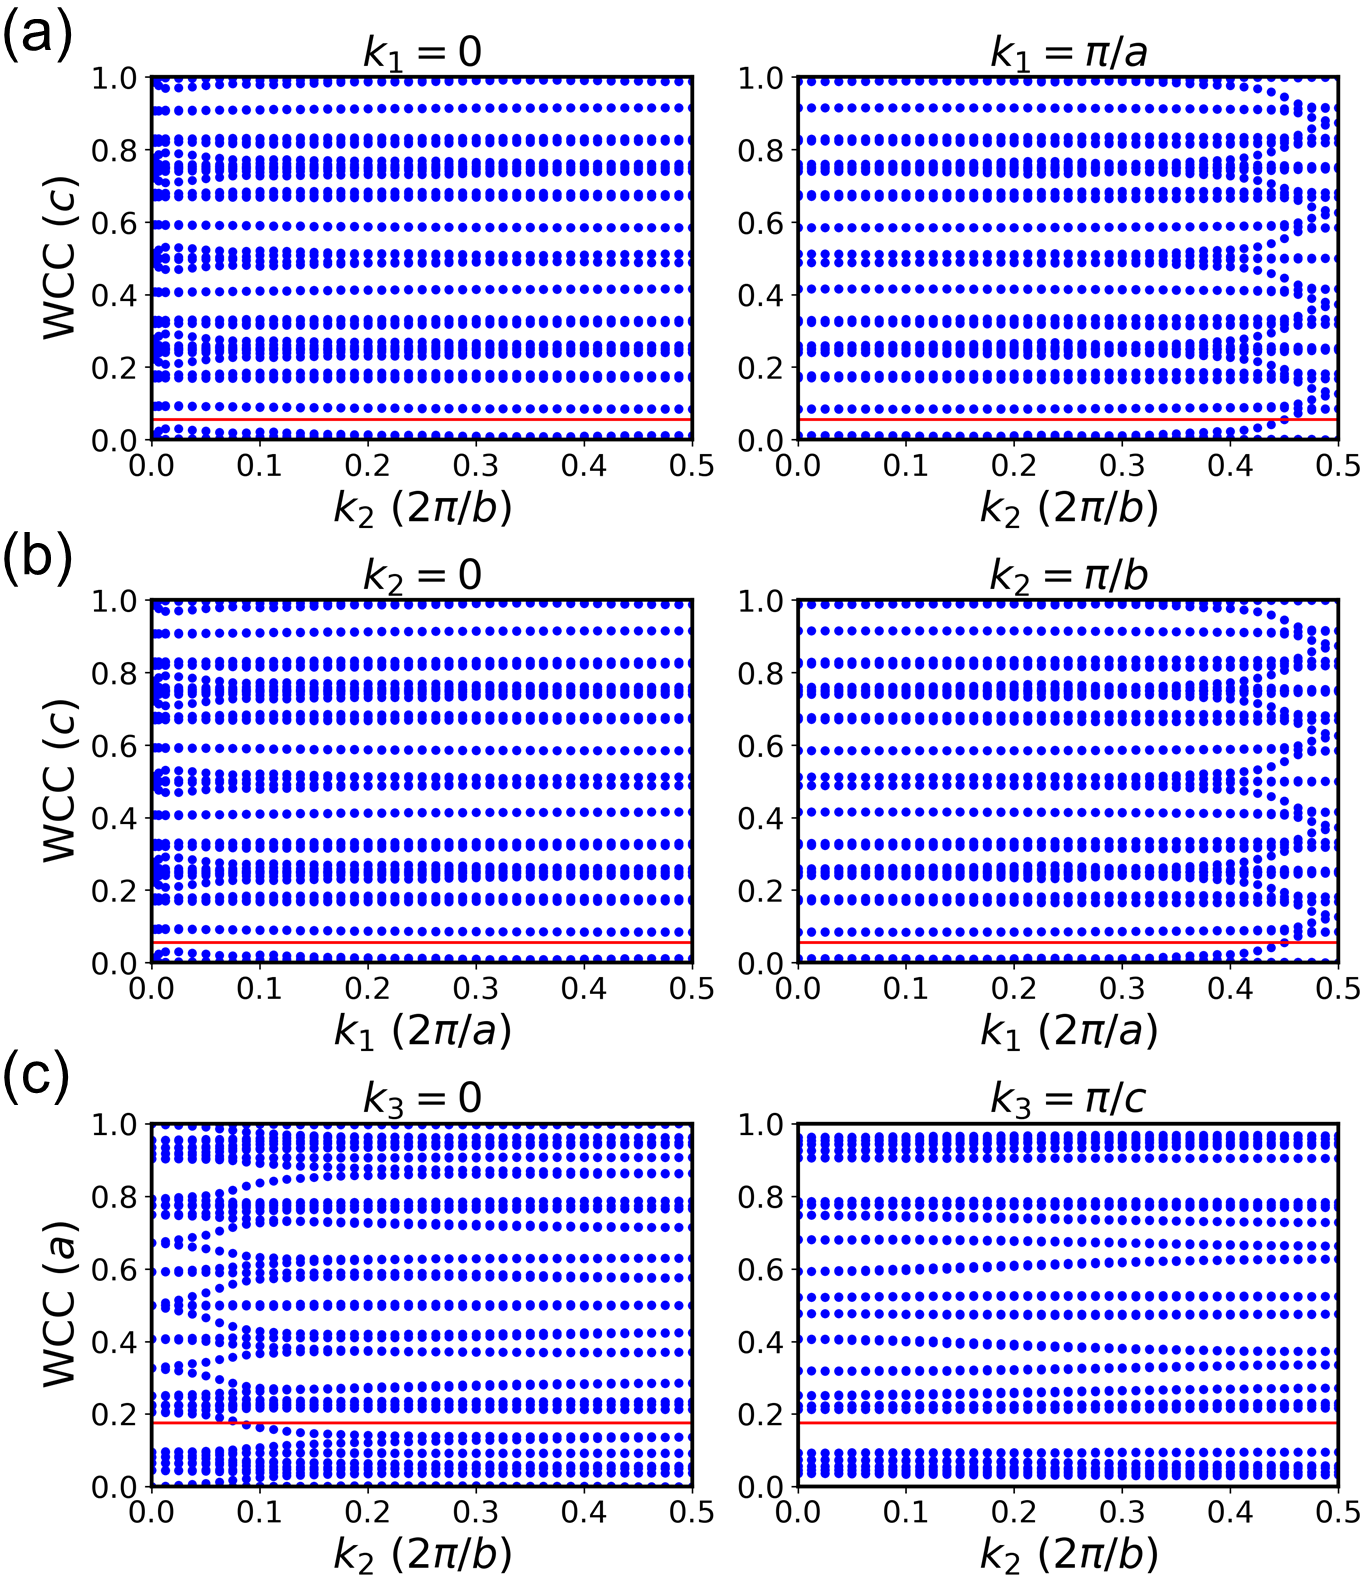
\includegraphics[width=0.8\textwidth]{ZrTe5_wcc.png}
        \caption[The evolutions of Wannier charge centers for six time-reversal invariant planes of ZrTe$_5$]{The evolutions of Wannier charge centers for six time-reversal invariant planes of ZrTe$_5$. (a) $Z_2=0$ for $k_1=0$ and $Z_2=1$ for $k_1=\pi/a$. (b) $Z_2=0$ for $k_2=0$ and $Z_2=1$ for $k_2=\pi/b$. (c) $Z_2=1$ for $k_3=0$ and $Z_2=0$ for $k_3=\pi/c$. Therefore, ZrTe$_5$ is a strong topological insulator with $Z_2$ indices = (1;110).}
        \label{ZrTe5_wcc}
    \end{figure}



	\begin{figure}[htbp]
        \centering
        \captionsetup{singlelinecheck = false, justification=justified}
        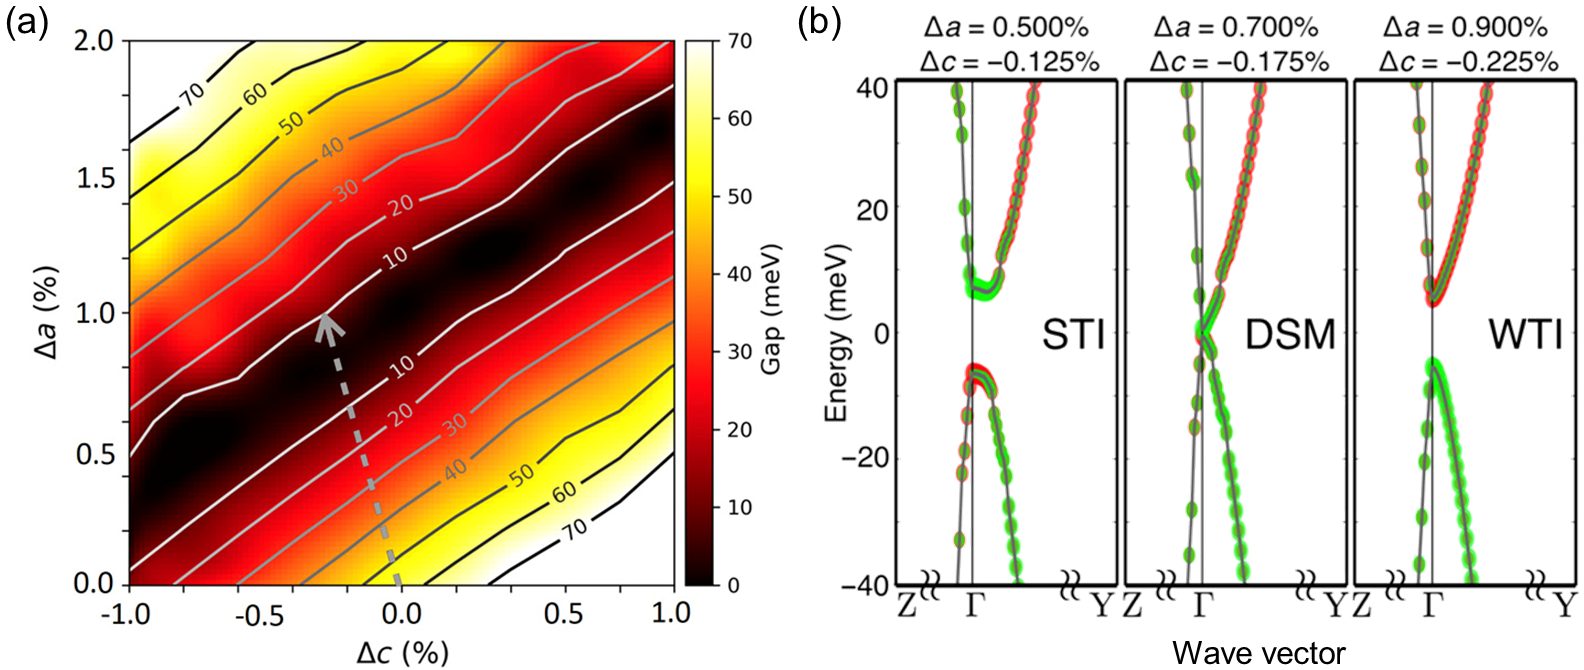
\includegraphics[width=0.95\textwidth]{ZrTe5_phase_transition.png}
        \caption[Topological phase transition in ZrTe$_5$ driven by uniaxial strain.]{(a) Bandgap $E_g$ at the $\Gamma$ point as functions of strains in $a$ and $c$ lattice directions. The dashed gray arrow indicates the anisotropic strain induced by a uniaxial stress along the a axis direction (b) Band structures for different strain states taken at points along the Poisson’s ratio path. These points (from left to right) correspond to STI, Dirac semimetal, and WTI, respectively. A band inversion involving Te$_d$ and Te$_z$ $p$ orbitals (shown as red and green colors, respectively) is seen in the STI phase.}
        \label{ZrTe5_phase_transition}
    \end{figure}

In order to achieve the topological phase transition by manipulating the lattice structure, it is important to know the response of the bandgap at $\Gamma$ point during the change in of lattice parameters. Fig. \ref{ZrTe5_phase_transition} (a) shows a contour map of the energy gap $E_g$ at $\Gamma$ as a function of $\epsilon_{aa}$ and $\epsilon_{cc}$, i.e., strain (\%) along the $a$ and $c$ lattice directions, calculated by density functional theory (DFT). It shows a V-shaped valley, with the minimum of the valley (corresponding to $E_g$ = 0) extending along the diagonal direction. $Z_2$ topological indices were also computed, and the $E_g$ = 0 line is the phase boundary between STI and WTI. Fig. \ref{ZrTe5_phase_transition} (a) reveals a highly anisotropic strain dependence of $E_g$: The steepest gradient of $E_g$ is along the direction in which $\epsilon_{aa}$ and $\epsilon_{cc}$ have opposite signs, as the case when an uniaxial stress is applied along the a lattice direction. In contrast, the strain induced by applying hydrostatic pressure corresponds to a trajectory that is almost parallel to the contour lines. The Poisson’s ratio of the anisotropic strain, $\epsilon_{cc}$/$\epsilon_{aa}$ = −0.25, induced by a-axis uniaxial stress, was obtained using a fully relaxed vdW-DFT calculation, and it is indicated as the gray arrow in Fig. \ref{ZrTe5_phase_transition} (a). It requires less than a percent of $\epsilon_{aa}$ to reach the WTI-STI phase boundary. We note that there is uncertainty in the DFT bandgap size for a given set of lattice constants. For example, several spectroscopy measurements reported $E_g$ as low as 10 meV, which is significantly lower than the calculated 60-meV bandgap at zero strain \cite{chen2017spectroscopic, jiang2017landau}. Hence, the actual strain required to pass through $E_g$ = 0 could be smaller.

	\begin{figure}[htbp]
        \centering
        \captionsetup{singlelinecheck = false, justification=justified}
        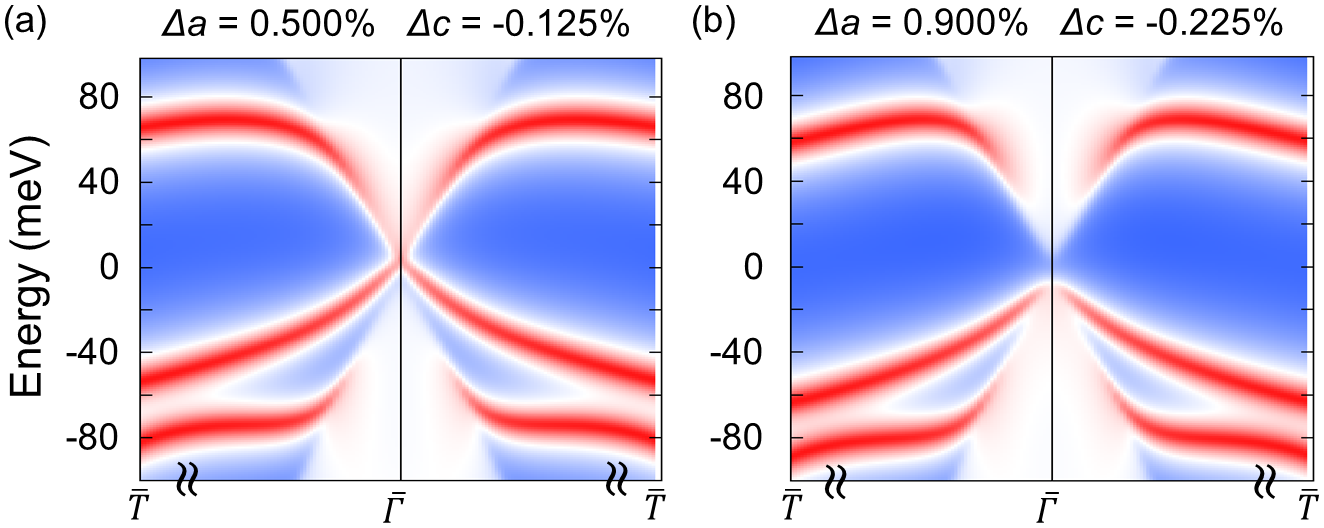
\includegraphics[width=0.95\textwidth]{ZrTe5_phase_transition_SS.png}
        \caption[Surface states around $\Gamma$ point on the (001) surface Brillouin zone in ZrTe$_5$ for STI and WTI phases.]{Surface states (represented by red lines) around $\Gamma$ point on the (001) surface Brillouin zone in ZrTe$_5$ for (a) STI and (b) WTI phases. (The white regions indicate the bulk bands.)}
        \label{ZrTe5_phase_transition_SS}
    \end{figure}

Based on the band structures of Fig. \ref{ZrTe5_phase_transition}(b), during the topological phase transition, one might observe the electrical transport properties, such as resistivity, will fall and rise again. This peculiar phenomenon was observed in the experiments done by Mutch {\it et al.} \cite{ZrTe5_2019}, and they also found that the positive longitudinal magnetoconductance also shows an unusual behavior that the value becomes maximal at the critical strain of phase transition. Besides, we further calculate the surface states around $\Gamma$ point in the (001) surface Brillouin zone [shown in Fig. \ref{ZrTe5_structure}(c)]. Figure \ref{ZrTe5_phase_transition_SS}(a) shows the topologically-protected surface states (represented by red lines) with a Dirac point at $\Gamma$ point for STI phase. For WTI phase, the surface states do not connect valence band and conduction band anymore. In summary, uni-axial strain is an effective tool to drive topological phase transition in small bandgap materials.

\vspace{12pt}
		
\noindent This section is based on our study published in {\it Science advances}, 5(8), p.eaav9771 \cite{ZrTe5_2019}.



\pagebreak
    
    %\subsection*{Structrual and Topological Phase Transitions in LaN}
    \addcontentsline{toc}{subsection}{Structrual and Topological Phase Transitions in LaN}
	{\centering
		\vspace{12pt} Structrual and Topological Phase Transitions in LaN \\
	    \par
	}

	%\section{\label{sec:level1}Introduction}
	
	Semimetallic lanthanum monopnictides such as LaAs, LaSb, and LaBi have attracted much attention because of their unusual extreme magnetoresistance due to electron-hole compensation~\cite{LaSb_XMR_tafti2015,LaBi_LaSb_topo_ARPES_niu2016,LaSb_LaBi_XMR_PNAS,LaAs_mBJ_XMR_yang2017}. These materials typically assume stable rock-salt structures, and they are promising for magnetic sensor and spintronics applications. Different from the above semimetals, LaP is found theoretically to be semiconducting with a narrow band gap ($< 0.1$ eV), and it displays high thermoelectric performance tunable by strain and pressure~\cite{LaP_1,LaP_2}. In addition to the intriguing magnetic and electronic behaviors of lanthanum monopnictides, researchers have recently paid attention to their non-trivial topological properties.
	 
    In the single-particle picture, topological bulk materials can be roughly categorized into topological semimetals (TSMs) and topological insulators (TIs). TSMs are characterized by topologically protected band crossings~\cite{TSM}; they include nodal semimetals such as Weyl and Dirac semimetals~\cite{yan2017,armitage2018}, as well as more exotic varieties like nodal-line semimetals~\cite{fang2016}, type-II Weyl semimetals~\cite{soluyanov2015}, and multifold fermions~\cite{fang2012,wieder2016,bradlyn2016}. For insulators with the time-reversal symmetry (TRS), topology arises from band inversion at TR-invariant momenta caused by strong spin-orbit coupling and can be classified by the $\mathbb{Z}_2$ indices~\cite{TI_hasan2010,qi2011}. The topologically non-trivial phases exhibit robust helical surface states with spin-momentum locking, which forbids back-scattering and thus renders new potential applications in low-dissipation devices.
	 
	 LaX (X = N, P, As, Sb, and Bi) lacks conducting $f$-electrons and preserves TRS, and their band structures also show an energy gap between valence and conduction bands at each $k$-point in the Brillouin zone (BZ). Hence, LaX still permits the $\mathbb{Z}_2$ classifications, even though some lanthanum monopnictides are semimetallic. Experimentally, the signature of topologically nontrivial (bulk) insulating phases can be determined by the conducting surface states near high symmetry points in the surface BZ, and they can be observed directly by angular-resolved photoemission spectroscopy (ARPES). In ambient conditions, LaBi is confirmed to be topologically nontrivial by several experimental groups~\cite{LaBi_topo_wu2016, LaBi_topo_ncomms13942, LaBi_topo_ARPES_lou2017, LaBi_LaSb_topo_ARPES_niu2016, LaBi_topo_PRB_feng2018, LaX_arpes_nummy2018}. In contrast, LaAs and LaSb are found to be topologically trivial in ARPES experiments~\cite{LaSb_ARPES_zeng2016, LaBi_LaSb_topo_ARPES_niu2016, LaX_arpes_nummy2018}. Recently, topological phase transitions (TPTs) are especially intriguing, because of the possibility to control different topological phases~\cite{TPT_2012, monserrat2017antiferroelectric, fan2017transition, ZrTe5_2019,sie2019ultrafast, vaswani2020light, PhysRevB.103.115207}. In LaAs and LaSb, pressure-induced TPTs have been proposed~\cite{LaAs_hydrostatic_pressure, LaSb_topo_transition_HSE_guo2017}. Since LaN and LaP are expected to show similar crystal and electronic structures as other lanthanum monopnictides, TPTs also may be achieved by uniaxial strain or hydrostatic pressure.

		%The topological nature of LaX was first studied theoretically by Zeng \textit{et al.}~\cite{LaX_TI_Lin}. Many theoretical studies have used density functional theory (DFT) to study the topological nature in LaX. However, traditional exchange-correlation functional based on local approximation like local-density approximation (LDA) and generalized gradient approximation (GGA) overly underestimate the gap between valence and conduction bands, which may lead to incorrect topological classification. For LaAs and LaSb, it is found that using modified Becke-Johnson (mBJ) functional \cite{mBJ_1, mBJ_2} or screened hybrid functionals with Hartree-Fock exact exchange energy\cite{HSE06} improves the band gap estimation and enable correct topological classification\cite{LaBi_LaSb_mBJ_guo2016, LaAs_hydrostatic_pressure,  LaSb_topo_transition_HSE_guo2017, LaAs_mBJ_XMR_yang2017, LaBi_LaSb_topo_dey2018}.
		
	\begin{figure*}
		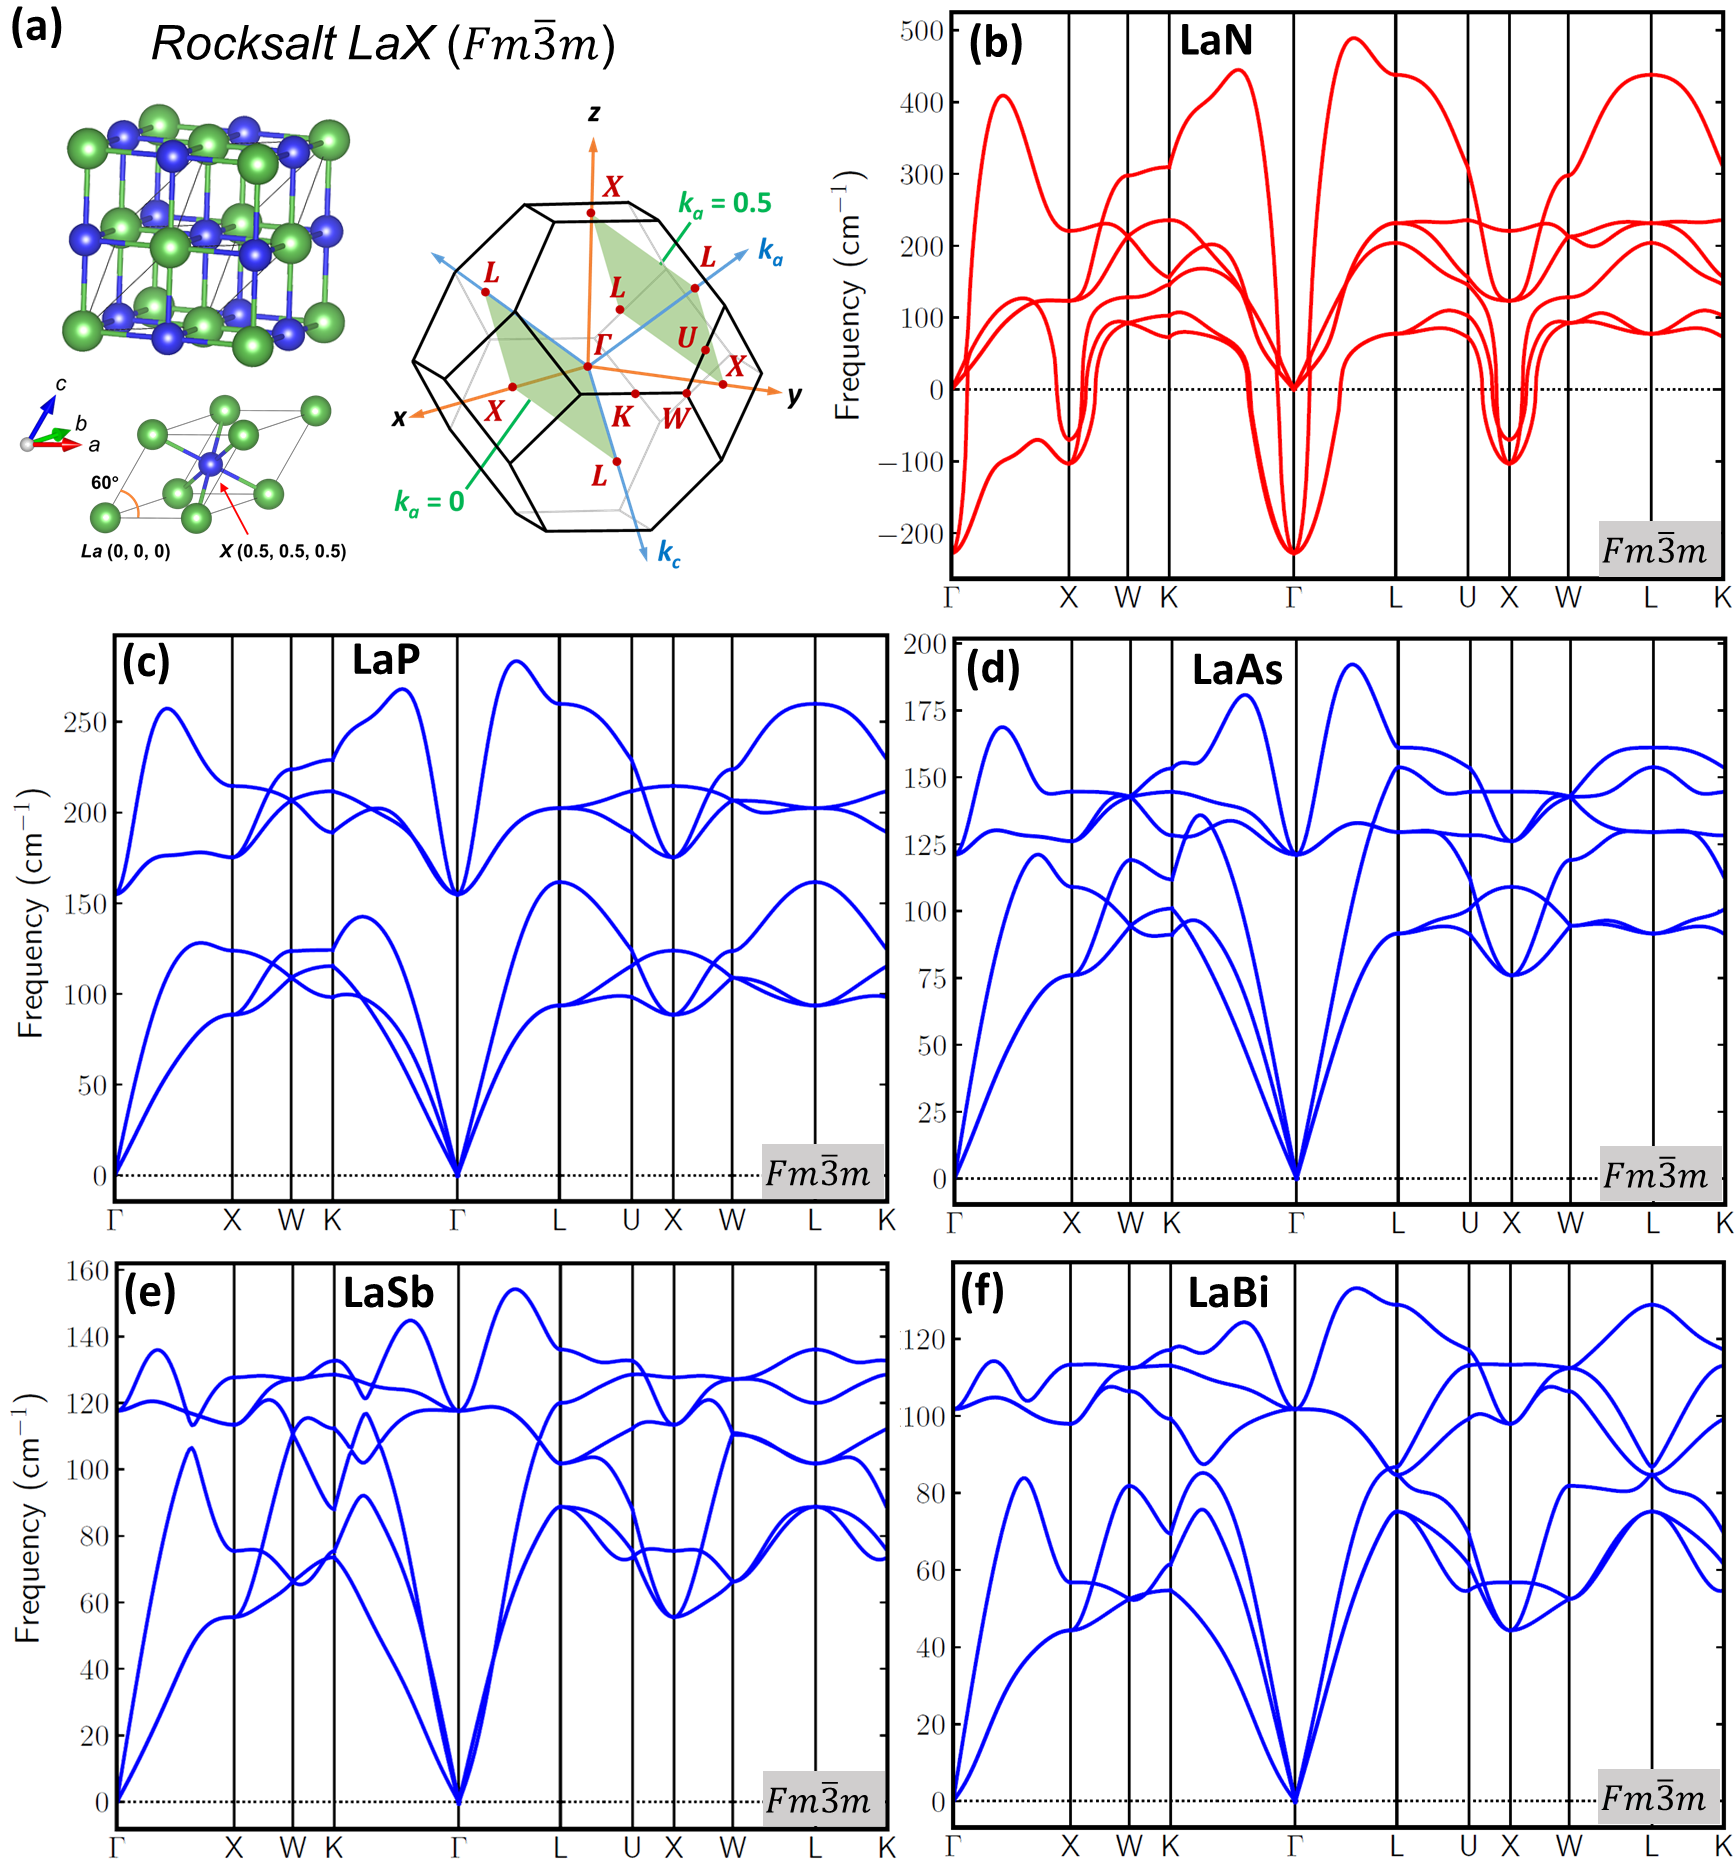
\includegraphics[width=\textwidth]{LaN_1.png}
        \captionsetup{singlelinecheck = false, justification=justified}
		\caption[Rock-salt crystal structure, Brillouin zone, and phonon dispersion of lanthanum monopnictides.]{(a) Rock-salt structure of LaX (with X = N, P, As, Sb, or Bi), and the corresponding Brillouin zone with projected (001) and (111) surfaces. (b)-(f) Phonon dispersions (without non-analytical term correction) of LaN, LaP, LaAs, LaSb, and LaBi, respectively. The imaginary phonon modes in (b) show that the rock-salt LaN is dynamically unstable at 0 K.}
		\label{fig:LaX_phonon}
	\end{figure*}
	
	In this paper, we use first-principles calculations to study the structural, electronic, and topological phase transitions of LaN. By re-examining the dynamic stabilities of all rock-salt LaX, we find that only LaN is dynamically unstable with imaginary phonon modes at zero temperature. Using evolutionary crystal structure prediction techniques, we find a new, dynamically stable structure of LaN with $P1$ symmetry. In our calculations, the $P1$-LaN also exhibits spontaneous electronic polarization, and it can undergo concomitant structural and ferroelectric transitions driven by temperature or pressure. 	The rest of the paper is organized as follows. First, we discuss the computational methods based on density functional theory, evolutionary crystal structure prediction, and {\it ab initio} molecular dynamics. Next, we present the theoretical results of structural, electronic, and topological properties of LaN under different temperature and pressure. We al discuss additionally topological phase transitions in rock-salt LaP, LaAs, and LaSb under hydrostatic pressure.
	Sec. IV concludes the paper by summarizing the conditions for stabilizing different phases under study. In the end,
	
%	\section{\label{sec:level1}Methods}
	
	Our density functional theory (DFT) calculations are conducted using the Vienna Ab initio Simulation Package (VASP)~\cite{kresse1996efficiency,kresse1996efficient, VASP_GPU_1, VASP_GPU_2}. In particular, the Perdew-Burke-Ernzerhof generalized gradient approximation (PBE-GGA)~\cite{PBE} functional and the projector augmented wave (PAW) method~\cite{PAW_1, PAW_2} are adopted. The wavefunctions are expanded in plane-wave basis sets with a kinetic energy cutoff of 500 eV, and a $\Gamma$-centered 11 $\times$ 11 $\times$ 11  Monkhorst-Pack $k$ mesh~\cite{MP} is used for the Brillouin zone sampling. In structure relaxation calculations, the convergence criteria for the force on each atom and the total energy are set to $1\times 10^{-3}$ eV/\r{A} and $1 \times 10^{-8}$ eV, respectively.
	
	% The obtained lattice constants from LaN to LaBi are 5.3076, 6.0496, 6.1925, 6.5466, and 6.6596 \r{A}, respectively. In experiments, (Scientific REPOrTS | 7: 6321: LaBi 6.5703(2) ) ( LaBi  6.5797 A) (PNAS June 21, 2016 113 (25) E3475-E3481: LaSb: 6.5008, LaBi:6.5799). (LaAs: 6.16707 -- PRB 96, 235128 (2017)) (LaP: 6.035 J. Phys.: Condens. Matter 19 (2007) 315220 C-G Duan et al )  (LaN:  5.295)
	% LDA: LaBi 6.493 (SCIentIfIC REPORTS | (2018) 8:14867) 
		
	To search for the zero-temperature (0 K) crystal structure of LaN, the \text{USPEX} package \cite{oganov2006crystal, glass2006uspex, lyakhov2013new} is used for crystal structure prediction (CSP). USPEX implements a highly efficient evolutionary algorithm for finding stable and meta-stable low-enthalpy structures corresponding to local minima in the potential energy surface. In our CSP calculations, 2-, 4-, and 8-atom unit cells are considered. The first generation of structures are randomly created. Subsequent generations are produced with 20\% from random structures and 80\% from heredity, soft mutation, and transmutation operators.
	
	The phonon dispersions at 0 K are calculated by the frozen-phonon approach with a $5\times 5 \times 5$ supercell (250 atoms) using VASP and PHONOPY~\cite{phonopy}. Here, VASP calculates the force on each atom in the supercell and provides the force information for PHONOPY, which in turn computes interatomic force constants and obtains phonon eigenvalues by diagonalizing the dynamical matrix. The atomic displacement is set as 0.02 \r{A}, and a 3 $\times$ 3 $\times$ 3 \textit{k}-mesh is employed in the self-consistency calculations. Since most of the rare-earth monopnictides are semimetallic, the non-analytical term correction is not included in our calculations.

	For finite-temperature phonon spectra, we adopt the temperature-dependent effective potential (TDEP)~\cite{TDEP} technique with \textit{ab initio} molecular dynamics (AIMD). The AIMD simulations use a time step of 2 fs and a total simulation length of 20 ps. We have checked the convergence of our results with respect to the total simulation time. The final 200 structures are then utilized to estimate the force constants via least-square fitting by using the ALAMODE package~\cite{Tadano_2014}.
	
	For electronic structure calculations, band orderings are essential for capturing the correct topological nature. However, standard DFT calculations based on local functionals like LDA or GGA typically underestimate the band gap, which may lead to an incorrect topological classification. To more adequately compute the band gap, we further apply an advanced non-local hybrid functional HSE06~\cite{HSE06} with spin-orbit coupling (SOC). Since hybrid DFT is computationally more demanding, we reduce the $k$ points to 9 $\times$ 9 $\times$ 9 and the cutoff energy to 400 eV (and we have checked that the band structure is quantitatively consistent with that obtained by using a 11 $\times$ 11 $\times$ 11 $k$ mesh and 500 eV energy cutoff). With the eigenvalues and eigenfunctions from hybrid-DFT, we construct maximally localized Wannier functions (MLWFs) and obtain corresponding \textit{ab-initio} tight-binding models using the Wannier90 package~\cite{wannier90}. We then use the WannierTools package~\cite{wanniertools} to identify topological $\mathbb{Z}_2$ indices by tracking the Wannier charge centers~\cite{z2pack}.
	
	
	%\section{\label{sec:level1}Results and Discussion}

	Several rare-earth monopnictides are known to be stabilized in the cubic rock-salt structure (space group No. 225, $Fm\bar{3}m$ symmetry), as shown in Fig. \ref{fig:LaX_phonon}(a). Indeed, a previous X-ray diffraction (XRD) experiment has reported the observation of rock-salt LaN~\cite{LaN_pressure_schneider2012}. However, a recent experiment using magnetron sputtering found only wurtzite and zinc blende structures for LaN~\cite{LaN_synthesis}. As a result, we begin by using DFT to examine the structural stability. We first fully relax the rock-salt structures for all lanthanum monopnictides using both LDA and GGA functionals without SOC. The resulting lattice parameters obtained by GGA (LDA) for LaX (with X ranging from N, P, As, Sb, to Bi) are 5.3076 (5.2140), 6.0496 (5.9377), 6.1925 (6.0656), 6.5466 (6.4019), and 6.6596 (6.5065) \r{A}, respectively. Compared with the experimental lattice parameters of 6.1670(7) \r{A} for LaAs~\cite{LaAs_mBJ_XMR_yang2017}, 6.5008 \r{A} for LaSb~\cite{LaSb_LaBi_XMR_PNAS}, and 6.5799 \r{A} for LaBi~\cite{LaSb_LaBi_XMR_PNAS}, GGA slightly overestimates the lattice parameters (with respective errors of 0.4\%, 0.7\%, and 1.2\%), while LDA underestimates them (with respective errors of -1.6\%, -1.5\%, and -1.1\%). We note that the SOC effect on lattice parameters is less than 0.1\%. Since overall the GGA results agree better with experiments, below we consider the fully relaxed structures obtained by GGA as the unstrained structures. 
	
	To examine the structural stabilities, we first compute the elastic constants using VASP~\cite{ELASTIC_VASP} to ensure that the Born-Huang criteria for cubic crystals are met~\cite{BORN-HUANG}: $C_{11}-C_{12} > 0$,  $C_{11}+2C_{12} > 0$, and $C_{44} > 0$. Our calculations indicate that all LaX rock-salt structures are mechanically stable. We next study the dynamical stability by calculating the phonon dispersion at 0 K. The phonon spectrum of LaN in Fig. \ref{fig:LaX_phonon}(b) contains soft modes with imaginary frequencies around the $\Gamma$ and $X$ points, which indicates the dynamical instability of LaN's rock-salt structure. Our LaN phonon dispersion calculated by a finite-displacement method is consistent with the study of G\"ok\"o\u{g}lu \textit{et al.}~\cite{LaN_phonon} based on density functional perturbation theory. For other lanthanum monopnictides, the phonon spectra in Figs. \ref{fig:LaX_phonon}(c)-(f) do not exhibit any soft mode, showing that the corresponding rock-salt structures are dynamically stable. This is also consistent with recent experiments~\cite{LaSb_ARPES_zeng2016, LaBi_LaSb_topo_ARPES_niu2016, LaX_arpes_nummy2018}. 
    We further note that in our electronic structure calculation using the HSE06 hybrid functional~\cite{HSE06}, unstrained rock-salt LaP is a semiconductor with an indirect band gap $\sim 82$ meV. Therefore, a longitudinal optical-transverse optical (LO-TO) phonon splitting near $\Gamma$ may be observed experimentally.


	\begin{figure}
	\centering
    \captionsetup{singlelinecheck = false, justification=justified}
	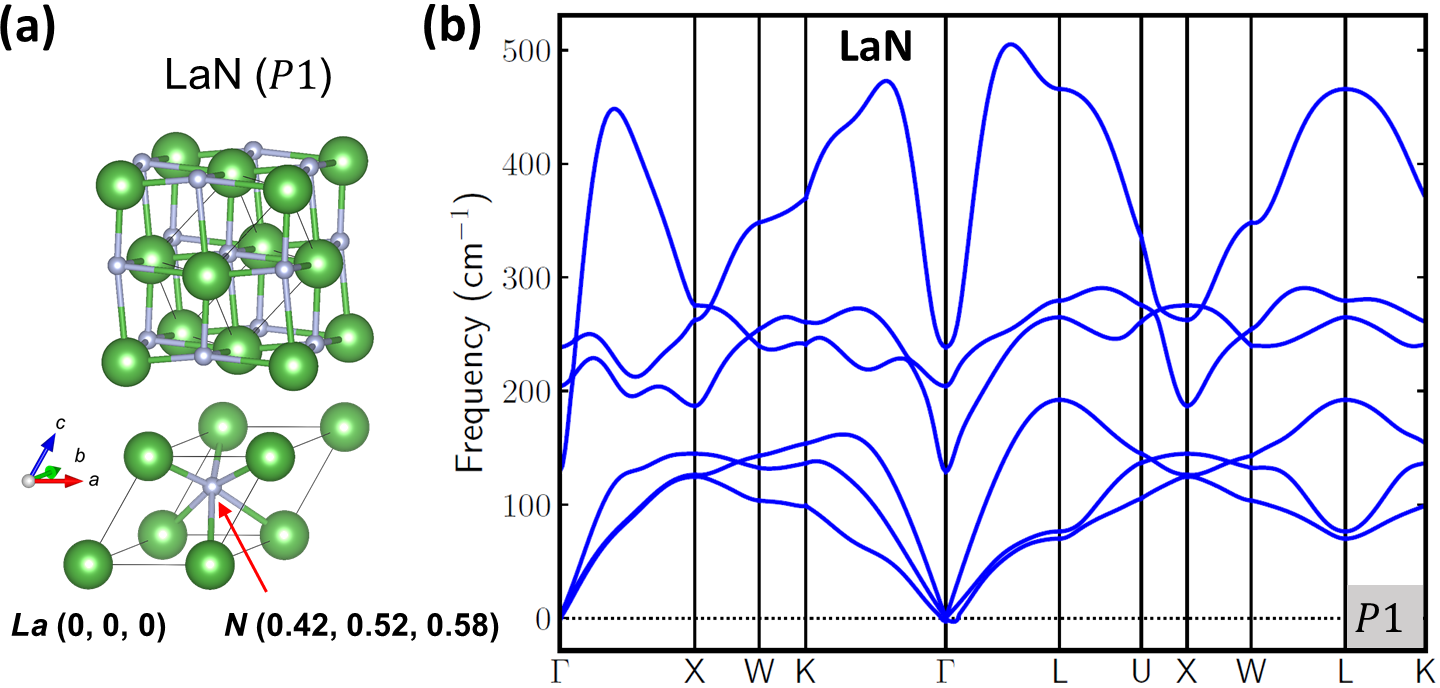
\includegraphics[width=0.8\linewidth]{LaN_2.png}
	\caption [Newly found LaN in distorted rock-salt structure and its phonon dispersion.]{(a) Distorted rock-salt structure obtained by evolutionary algorithm for LaN. This structure lacks an inversion center and belongs to space group No. 1 (\textit{P1} symmetry). The lattice parameters are a = 3.7245 \r{A}, b = 3.8192 \r{A}, c = 3.7557 \r{A}, $\alpha$ = 58.8990$^{\circ}$, $\beta$ = 61.3750$^{\circ}$, and $\gamma$ = 59.7033$^{\circ}$. The Wyckoff positions are La (0, 0, 0) and Na (0.42, 0.52, 0.58). (b) Phonon dispersion of the $P1$-LaN structure. The labelings of high-symmetry points are based on the fcc lattice. The absence of imaginary phonon mode indicates that $P1$ LaN is dynamically stable at 0 K.}
	\label{fig:LaN_2}
	\end{figure}
	
	The imaginary phonon modes in rock-salt LaN imply a different stable crystal structure at 0 K. Using the evolutionary algorithm implemented in \text{USPEX} \cite{oganov2006crystal, glass2006uspex, lyakhov2013new}, we conduct crystal structure searches at 0 K and find a lower-symmetry structure with space group No. 1 ($P1$ symmetry) shown in Fig. \ref{fig:LaN_2}(a) as the ground state. The lattice parameters of the primitive cell are a = 3.7245 \r{A}, b = 3.8192 \r{A}, and c = 3.7557 \r{A}. The angles between them are $\alpha$ = 58.8990$^{\circ}$, $\beta$ = 61.3750$^{\circ}$, and $\gamma$ =   59.7033$^{\circ}$. The Wyckoff positions for La and N are (0, 0, 0) and (0.42, 0.52, 0.58), respectively. This structure can be regarded as a distorted rock-salt structure, where the N position is slightly shifted away from the more symmetric (0.5, 0.5, 0.5) position. Figure \ref{fig:LaN_2}(b) shows the corresponding phonon dispersion, and the absence of imaginary mode indicates that $P1$-LaN is dynamically stable at 0 K.


	To ensure that $P1$-LaN is indeed the ground state structure, we also compute the total energy versus volume for LaN in five different crystal structures: the low-symmetry structure $P1$ (space group No. 1), rock salt $Fm\bar{3}m$ (No. 225), PbO-like tetragonal structure $P4/nmm$ (No. 129), wurtzite $P6_3mc$ (No. 186), and zinc blende $Fm\bar{4}3m$ (No. 216). As shown in Fig. \ref{fig:LaN_3}(a), the $P1$ structure has the lowest total energy, which is 29 meV (per formula unit of LaN) lower than that of the rock-salt structure. The lowest possible total energy of the wurtzite structure is also 16 meV (per formula unit) lower than that of the rock-salt structure. In the phonon dispersions for the wurtzite and zinc-blende structures shown in Fig. \ref{fig:LaN_4}, both of them are dynamically stable at 0 K. Our theoretical results thereby support the recent experimental findings of synthesized wurtzite and zinc-blende LaN~\cite{LaN_synthesis}.

	\begin{figure}
		\centering
        \captionsetup{singlelinecheck = false, justification=justified}
		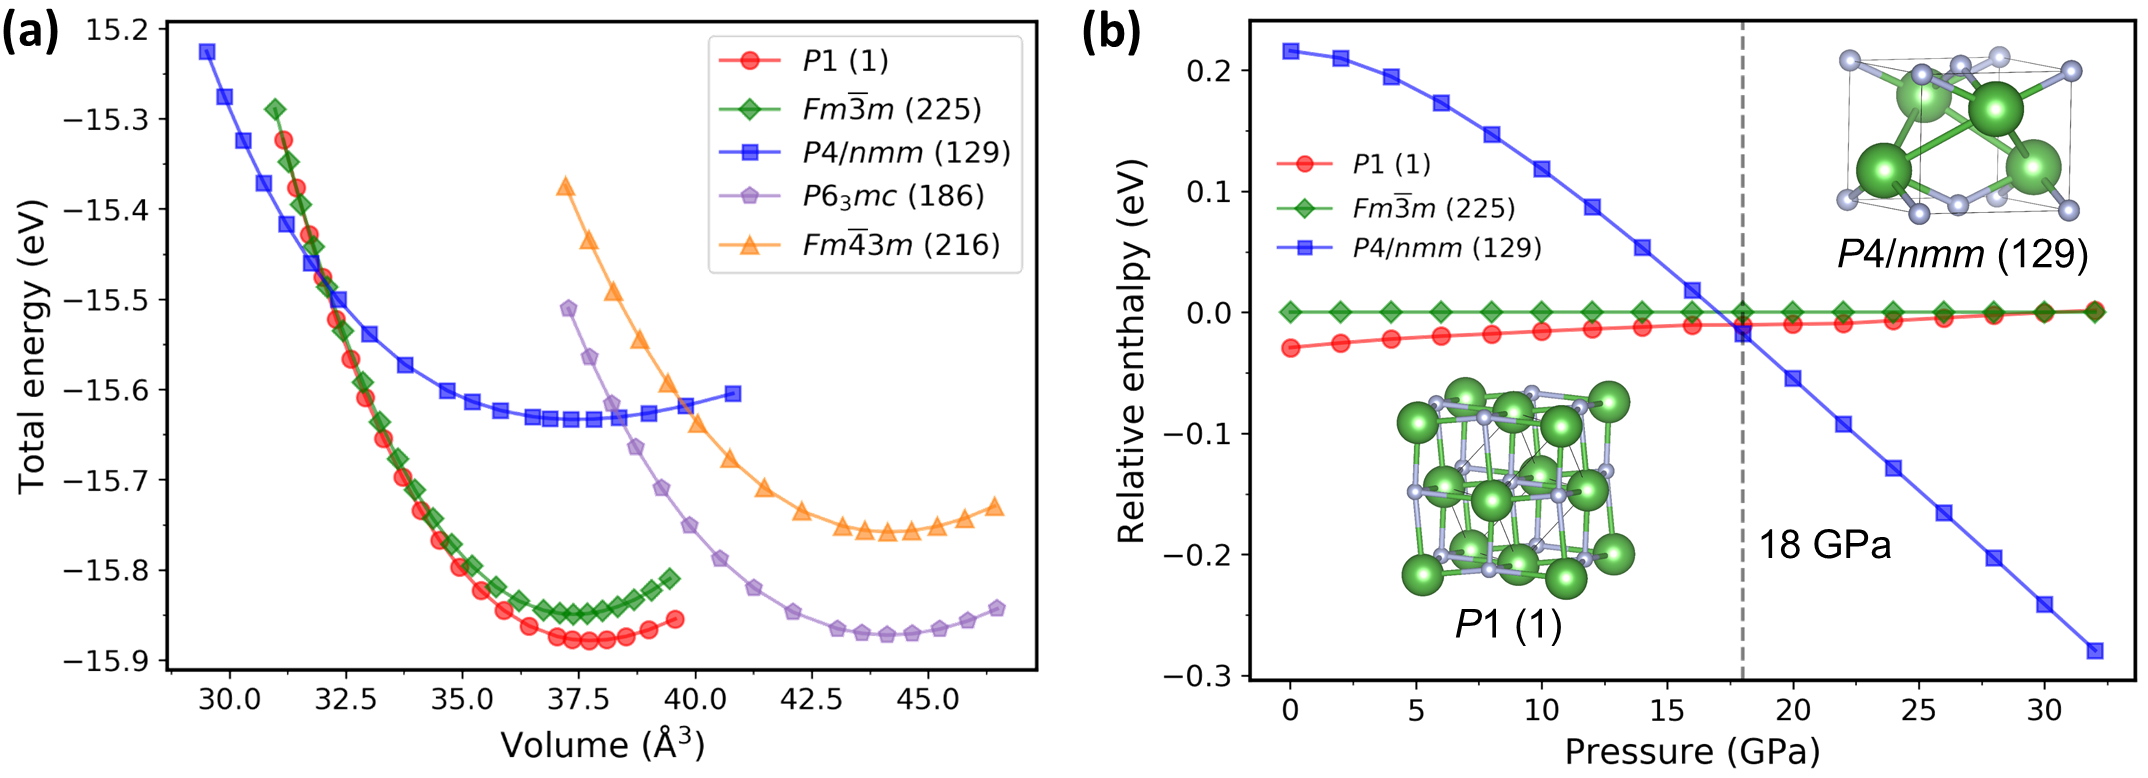
\includegraphics[width=\linewidth]{LaN_3.png}
		\caption [Total energy and relative enthalpy of LaN in different structures.]{(a) Total-energy versus volume curves of LaN in different crystal symmetries, including the low-symmetry structure $P1$ (space group No. 1), rock salt $Fm\bar{3}m$ (No. 225), PbO-like tetragonal structure $P4/nmm$ (No. 129), wurtzite $P6_3mc$ (No. 186), and zinc blende $Fm\bar{4}3m$ (No. 216). (b) Relative formation enthalpy as a function of pressure using rock-salt LaN as the reference. The result indicates a pressure-induced structure transition from $P1$ to $P4/nmm$ symmetry near 18 GPa.}
		\label{fig:LaN_3}
	\end{figure}

	\begin{figure}
		\centering
        \captionsetup{singlelinecheck = false, justification=justified}
		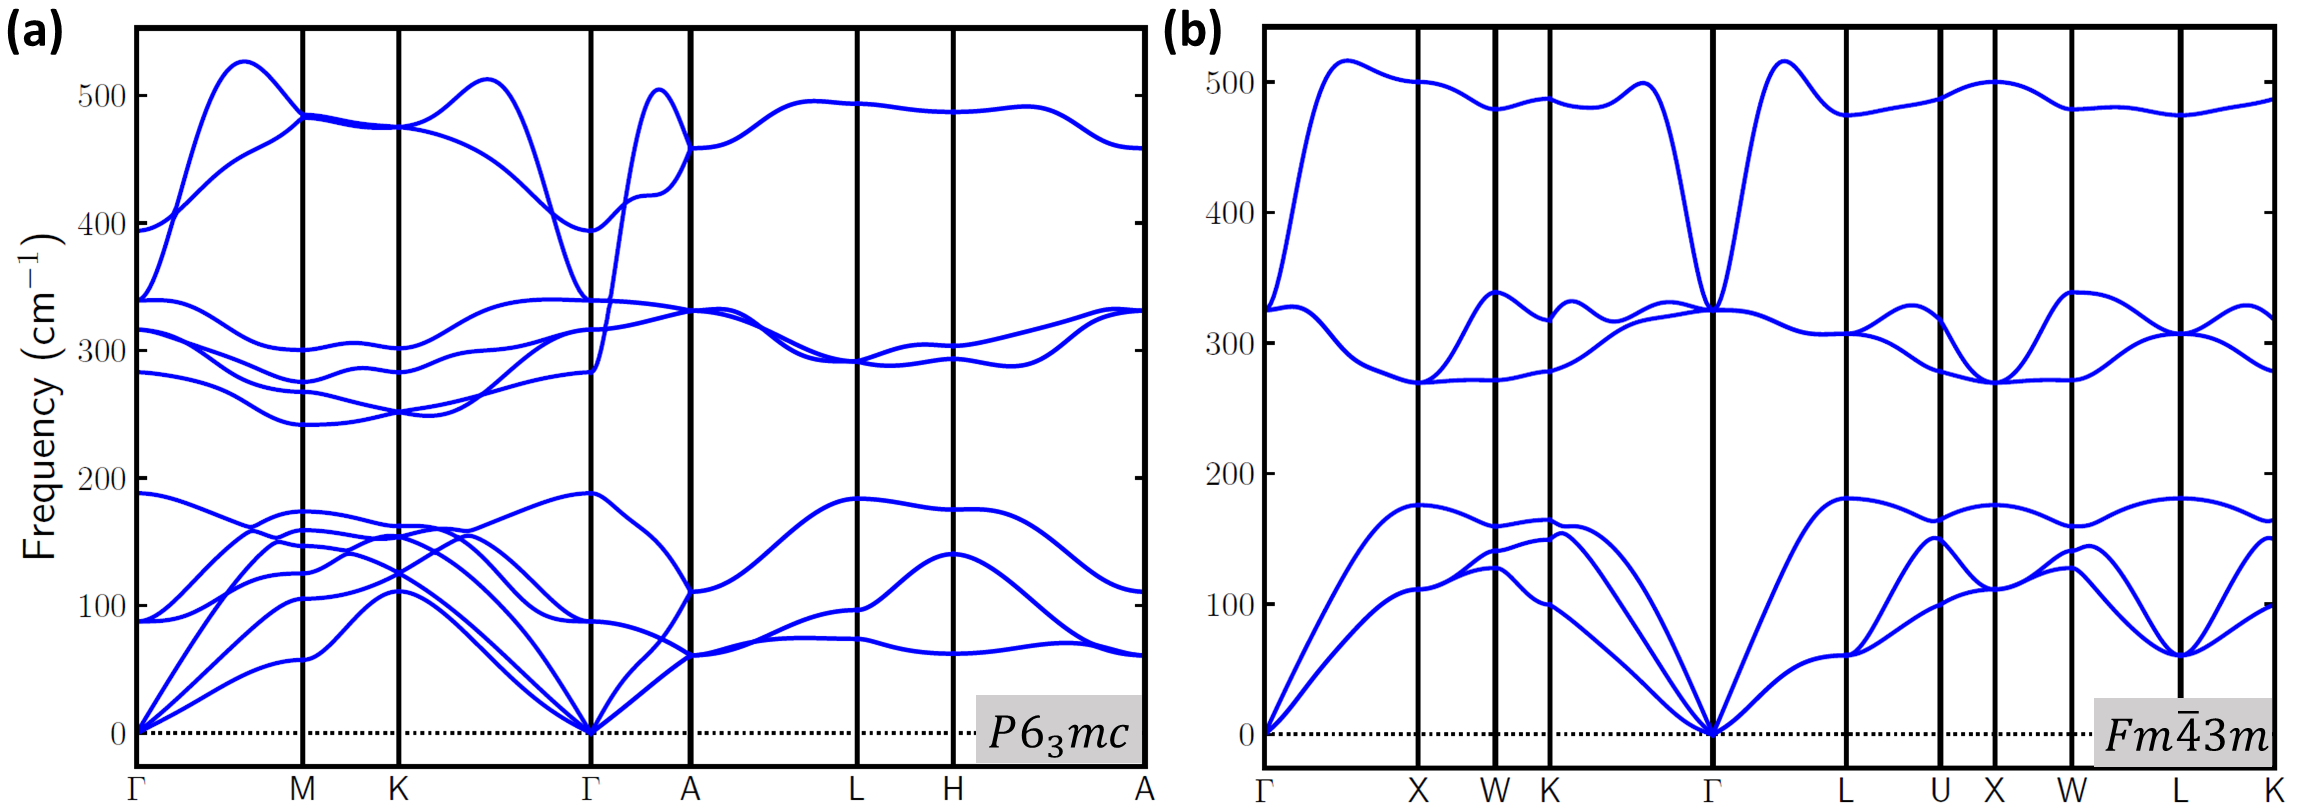
\includegraphics[width=1.0\linewidth]{LaN_4.png}
		\caption[Phonon dispersions of LaN in wurtzite and zinc-blende structures]{Phonon dispersions of LaN in (a) wurtzite and (b) zinc-blende structures, and both of them are dynamically stable.}
		\label{fig:LaN_4}
	\end{figure}


	Figure \ref{fig:LaN_3}(a) also shows that the total energy-volume curves of $P1$ and $P4/nmm$ intersect around 32 \r{A}$^3$. Therefore, applying external pressure can favor the PbO-like $P4/nmm$ tetragonal structure. Figure \ref{fig:LaN_3}(b) shows the calculated relative formation enthalpy as a function of pressure, using the rock-salt $Fm\bar{3}m$ structure as the reference. The result indicates that when the external pressure is below 18 GPa, $P1$-LaN has the lowest enthalpy. Above 18 GPa, $P4/nmm$-LaN becomes the lowest enthalpy structure. In other words, our DFT calculations suggest a pressure-induced structural phase transition from $P1$ to $P4/nmm$ symmetry in LaN near 18 GPa at 0~K. Our predicted transition pressure is similar to that from a previous theoretical study by Mukherjee {\it et al.}, who proposed a transition pressure of 19 GPa for LaN to transit from $Fm\bar{3}m$ to $P4/nmm$ symmetry~\cite{LaN_pressure_theory}. The theoretical results are also consistent with the experimental finding by Schneider {\it et al.}, who observed the $Fm\bar{3}m$ structure in ambient conditions, and it undergoes a phase transition to the PbO-like $P4/nmm$ tetragonal structure at $\sim 22.8$ GPa~\cite{LaN_pressure_exp}.


	
	On the other hand, although our DFT calculation predicts a stable $P1$-LaN at 0 K, this structure has not been reported before. As mentioned above, the rock-salt $Fm\bar{3}m$-LaN is generally acknowledged in the literature as the correct structure in ambient conditions. These results imply that LaN may exhibit a temperature-induced structural transition from $P1$ to $Fm\bar{3}m$ symmetry. In fact, the situation here for LaN is very similar to that in ferroelectric materials GeSe and GeTe~\cite{GeSe,GeTe_Xia}. There, the structural transitions induced by temperature are usually accompanied by ferroelectric transitions. For example, rhombohedral $\alpha$-GeTe (space group No. 160, $R3m$ symmetry) undergoes a ferroelectric transition and a structural change to rock-salt $\beta$-GeTe (No. 225, $Fm\bar{3}m$) near 700 K~\cite{GeTe_Xia}. An important signature of ferroelectric material is the double-well potential energy surface (PES), which can be obtained by the nudged elastic band method. Motivated by the similarity between GeTe and LaN, we compute the spontaneous electric polarization of $P1$-LaN based on the modern theory of polarization~\cite{modern_polarization}. Figure \ref{fig:LaN_5}(a) shows the potential energy as a function of polarization, which exhibits a double-well energy landscape. In our calculations, $P1$-LaN has a switching barrier of 53 meV per formula unit, and the ground state structure displays a net polarization of 36 $\mu$C/cm$^2$. Therefore, LaN is likely to undergo a concurrent ferroelectric transition and structural change from $P1$ to $Fm\bar{3}m$ symmetry when temperature is increased.

	
	\begin{figure}
		\centering
        \captionsetup{singlelinecheck = false, justification=justified}
		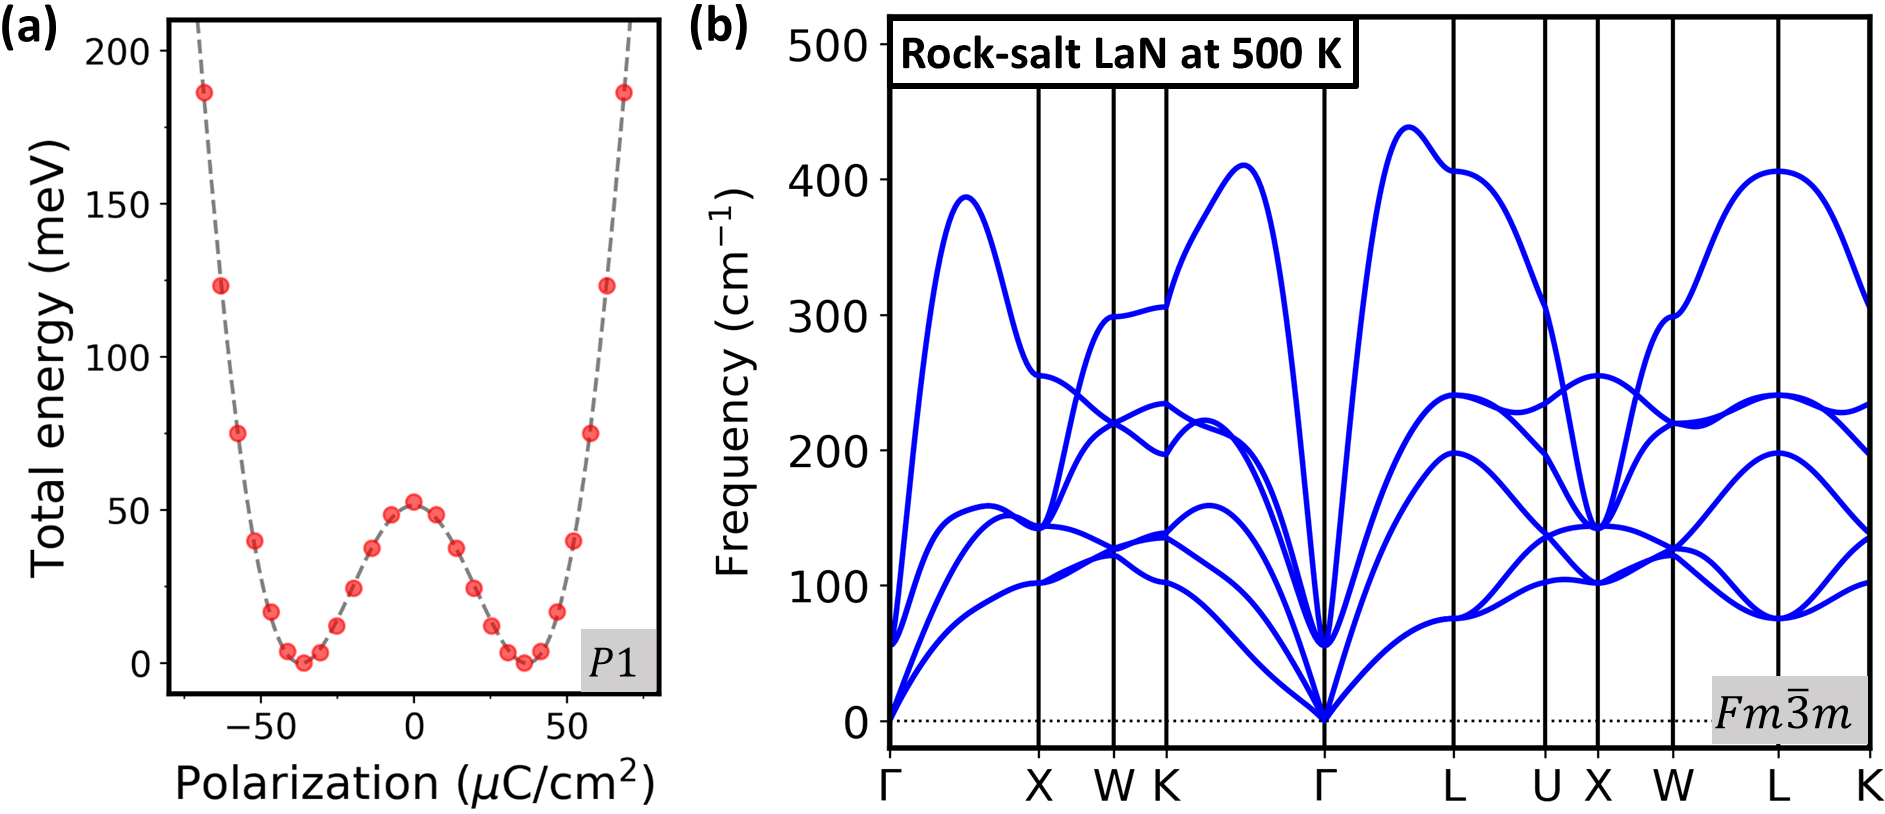
\includegraphics[width=1.0\linewidth]{LaN_5.png}
		\caption[Double-well potential energy versus polarization in $P1$-LaN and renormalized phonon dispersion of rock-salt LaN at 500 K]{(a) Double-well potential energy versus polarization in $P1$-LaN using the ground state energy as a reference, where the ground state shows a spontaneous polarization of 36 $\mu$C/cm$^2$. The gray dashed line is the fitting function up to 6$th$ order. (b) Renormalized phonon dispersion of rock-salt ($Fm\bar{3}m$) LaN at 500 K. Compared to the phonon dispersion at 0 K in Fig. \ref{fig:LaX_phonon}(b), the absence of imaginary mode here shows that rock-salt LaN can be stabilized at high temperature.}
		\label{fig:LaN_5}
	\end{figure}
	

	To confirm our conjecture that rock-salt LaN can be stabilized at high temperature, we calculate its finite-temperature (or renormalized) phonon dispersion. To include anharmonic effects, we use the TDEP method~\cite{TDEP} to obtain the effective 2nd-order force constants and fit them via AIMD simulations. Figure \ref{fig:LaN_5}(b) shows the renormalized phonon dispersion of rock-salt LaN at 500 K. No imaginary mode exists, indicating the dynamical stability of rock-salt LaN at high temperature. Here, we do not attempt to discuss the exact critical temperature, because it is computationally demanding to calculate and also depends on the chosen DFT functional.
	
	Here, we do not attempt to discuss the exact critical transition temperature, because it is computationally demanding to calculate and also depends on the chosen DFT functional. In particular, our phonon dispersions computed with the PBE functional still contain negative frequencies of -60 and -44 cm$^{-1}$ at the $\Gamma$ point at temperatures 100 K and 300 K, respectively. We have also calculated the phonon dispersion at 300 K using the LDA functional, and the result shows that the negative phonon frequency at 300 K is reduced to only -19 cm$^{-1}$.
	


	\begin{figure*}[ht!]
		\centering
        \captionsetup{singlelinecheck = false, justification=justified}
		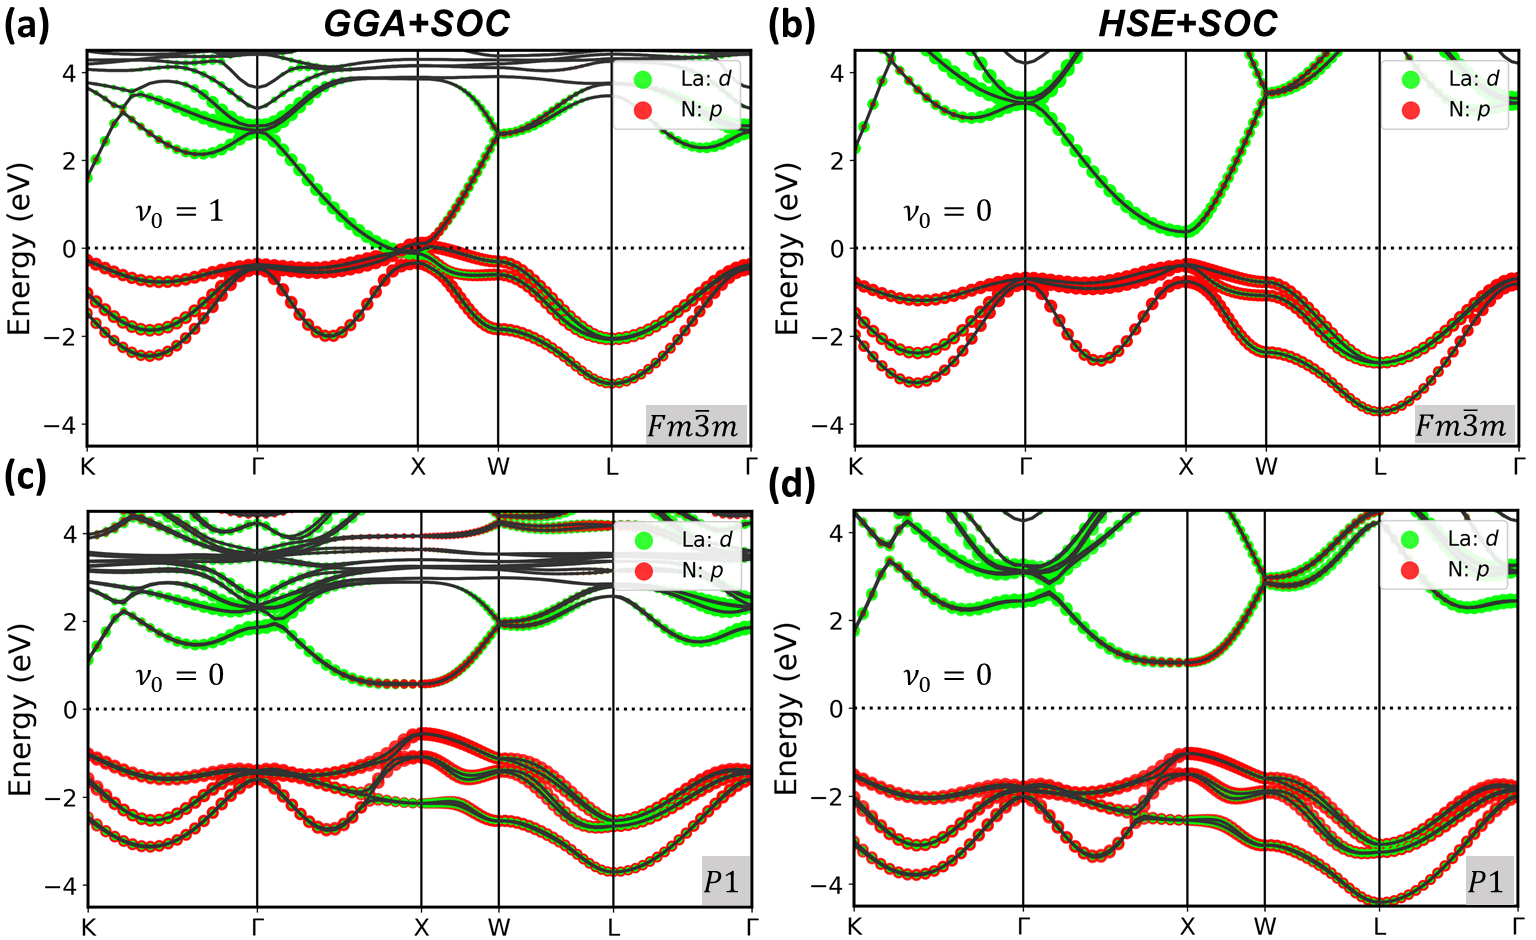
\includegraphics[width=0.95\textwidth]{LaN_6.png}
		\caption[Band structures based on PBE-GGA functional and HSE hybrid functional of LaN in $P_1$ and $Fm\bar{3}m$ structures]{Electronic band structures with spin-orbit coupling (SOC) and $\mathbb{Z}_2$ topological indices for rock-salt LaN, calculated with (a) the PBE-GGA functional and (b) the HSE06 hybrid functional. (c)-(d) are similar plots as (a)-(b), but for $P1$ LaN. The labelings of high-symmetry points are based on the fcc lattice. The Fermi level (horizontal dotted line) is set to 0 eV. GGA typically underestimates the band gap, which can be corrected by a more advanced hybrid functional.}
		\label{fig:LaN_6}
	\end{figure*}

	We next shift our focus to electronic and topological properties. In a 3D system with time reversal symmetry (TRS), band topology can be characterized by the $\mathbb{Z}_2$ indices ($\nu_0$; $\nu_1, \nu_2, \nu_3$), if an energy gap exists at each $k$-point in the BZ~\cite{fu2007}. A strong topological insulator (STI) has a strong index $\nu_0$ = 1 with an odd number of Dirac cones on any surface. In contrast, the weak TI phase has $\nu_0$ = 0, and it can be regarded as a stacking of 2D quantum spin Hall~\cite{maciejko2011} layers along the ($\nu_1,\nu_2,\nu_3$) ``mod 2'' reciprocal lattice vector~\cite{fu2007}. Therefore, the weak indices ($\nu_1,\nu_2,\nu_3$) depend on the choice of unit cell, and here they are defined by the primitive crystal structure. To understand the $\mathbb{Z}_2$ topology of a system with both TRS and inversion symmetries~\cite{fu2007topological}, one can study simply the product of the parity eigenvalues of the occupied bands at the time-reversal invariant momenta (TRIM). In the rock-salt structure, the TRIM include 1 $\Gamma$, 3 $X$, and 4 $L$, as shown in Fig. \ref{fig:LaN_2}(b). Therefore, only a sign change in the parity eigenvalue at $\Gamma$ or $X$ point can lead to a change in $\nu_0$ (i.e. a STI topological phase transition). On the other hand, the three weak indices depend on 2 (even number) $X$ and 2 (even number) $L$ points, and thereby they are always 0. 
	
		%At ambient condition among La$X$, we find only LaBi is nontrivial with products of parities at TRIM: $+$ ($\Gamma$), $-$ ($X$), $+$ ($L$), which is consistent with previous studies [ref]. For the trivial LaP, LaAs [ref], and LaSb [ref], their parity products at TRIM are $+$ ($\Gamma$), $+$ ($X$), $+$ ($L$). In the light of the similarity in La$X$'s band dispersions, the ``$-$'' sign at $X$ in LaBi implies the band inversion occurs at $X$.

	\begin{figure*}[ht!]
	    \centering
        \captionsetup{singlelinecheck = false, justification=justified}	
		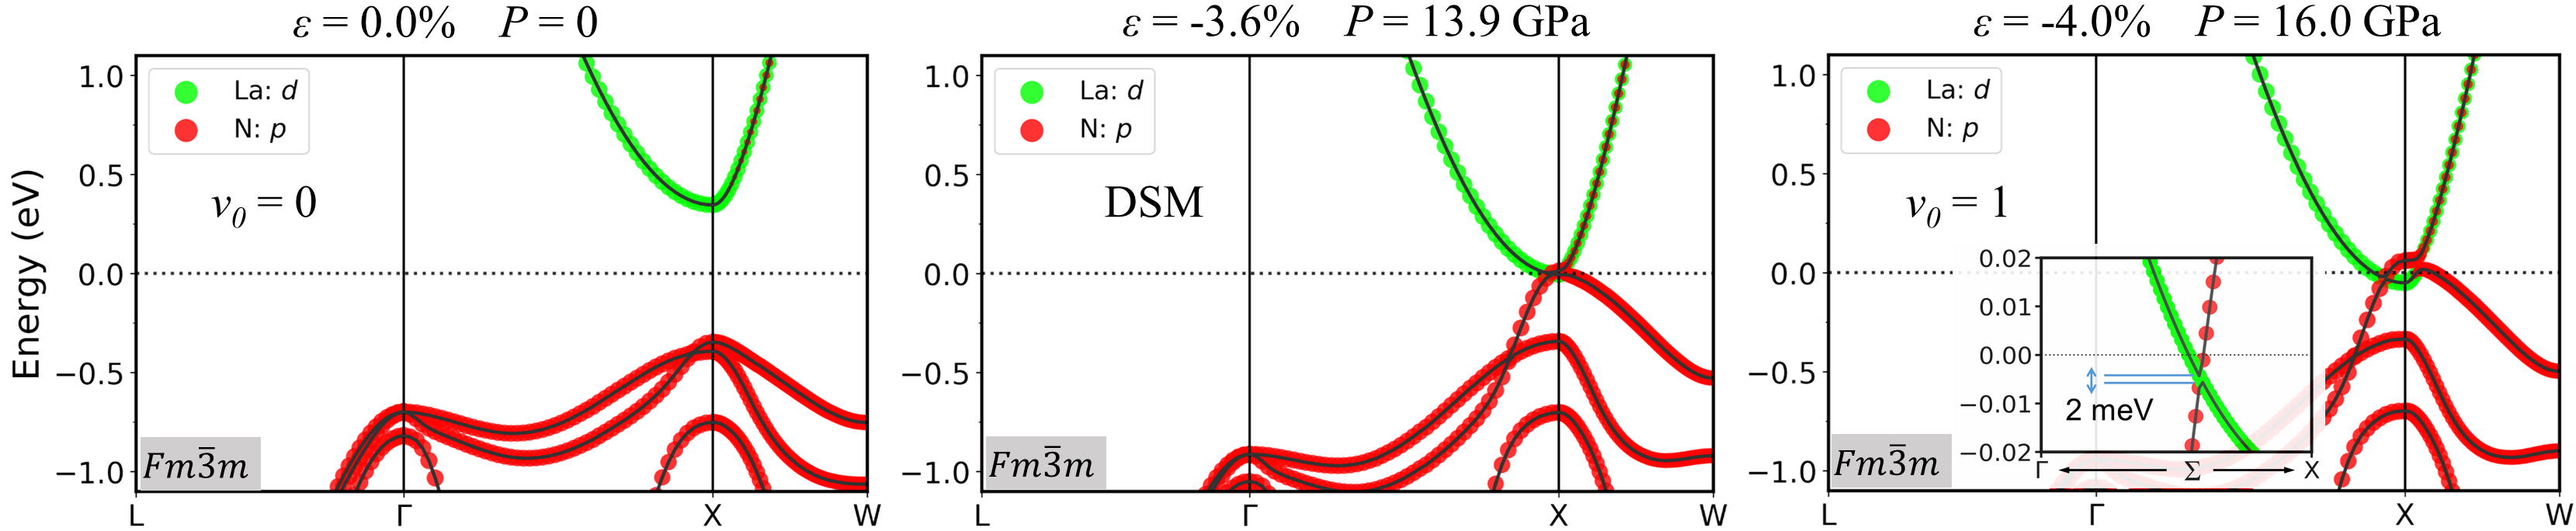
\includegraphics[width=\textwidth]{LaN_7.png}
		\caption[Topological phase transition driven by hydrostatic pressure in rock-salt LaN]{Electronic band structures and $\mathbb{Z}_2$ topological indices of rock-salt LaN under different strain $\varepsilon$ and corresponding pressure $P$. Left: $P$ = 0, trivial insulator ($\nu_0$ = 0). Middle: $P$ = 13.9 GPa, Dirac semimetal (DSM). Right: $P$ = 16.0 GPa, strong topological insulator ($\nu_0$ = 1). The results show a pressure-driven topological phase transition in rock-salt LaN.}
		\label{fig:LaN_7}
	\end{figure*}	


	The electronic band topology of LaX was first investigated by Zeng \textit{et al.} using the DFT+U method~\cite{LaX_TI_Lin}, which however does not fix the issue of underestimating LaX's band gaps and may lead to incorrect topological classifications. Later DFT studies based on the modified Becke-Johnson (mBJ) meta-GGA functional~\cite{mBJ_1, mBJ_2} or screened hybrid functionals~\cite{HSE06} have addressed this issue, and thereby their topological classifications are potentially more appropriate~\cite{LaBi_LaSb_mBJ_guo2016,LaAs_mBJ_XMR_yang2017, LaBi_LaSb_topo_dey2018}. Here, we study the electronic band structures using both PBE-GGA~\cite{PBE} and HSE06~\cite{HSE06}. For rock-salt LaN, the GGA band structure in Fig. \ref{fig:LaN_5}(a) shows a semimetal and a topologically non-trivial STI phase ($\nu_0 = 1$) with band inversion at the $X$ point. However, this STI assignment is potentially incorrect, due to an underestimation of the overall gap between valence and conduction bands. In contrast, the more advanced HSE06 band structure in Fig. \ref{fig:LaN_6}(b) shows that rock-salt LaN is a semiconductor with a direct band gap $\sim 0.8$ eV at the $X$ point, and the material is topologically trivial ($\nu_0 = 0$). We also calculate the band structures of $P1$-LaN. As shown in Figs. \ref{fig:LaN_5}(c)-(d), the PBE-GGA and HSE06 results both show a semiconducting phase with a direct band gap $\sim 1.1$ and 2.2 eV, respectively. The orbitally-resolved band structures of $P1$-LaN show contributions from nitrogen's $p$-orbitals near the conduction band minimum. However, we note that this apparent ``band inversion" at the $X$ point is not related to SOC. Instead, the orbital hybridization is caused by the lower-symmetry of the distorted $P1$ structure. Due to the absence of inversion symmetry, the topological nature cannot be simply determined from the parity eigenvalues of the TRIM. Instead, here $\nu_0$ is calculated by tracking directly the Wannier charge centers, and $P1$-LaN is found to be topologically trivial ($\nu_0 = 0$).

	Finally, we study pressure-induced topological phase transitions (TPTs) in LaX. Recently, researchers have reported that the band topology of LaAs and LaSb can be controlled by pressure~\cite{LaAs_hydrostatic_pressure,  LaSb_topo_transition_HSE_guo2017}. External pressure can modify the band gap, leading to a band inversion between valence and conduction bands. Following a similar idea, here we calculate the HSE06 band structures of LaN under external pressure. As shown in the left panel of Fig. \ref{fig:LaN_7}, the unstrained (ambient-condition) rock-salt LaN is topologically trivial ($\nu_0$ = 0). When a hydrostatic pressure of 13.9 GPa is applied, the energy gap is closed at the $X$ point, and rock-salt LaN becomes a Dirac semimetal (middle panel of Fig. \ref{fig:LaN_7}). When the external pressure is above 13.9 GPa, a band inversion occurs (right panel of Fig. \ref{fig:LaN_7}), and the material becomes a STI ($\nu_0$ = 1). Since inversion is preserved across the transition, the Dirac semimetal appears exactly and only at the TPT, and must necessarily appear at a TRIM~\cite{murakami2007,murakami2008}, here the three $X$ points in the BZ. We note that in the non-trivial STI phase, there is a very small gap $\sim$ 2 meV (the $\Sigma$ point in the insert, right panel of Fig. \ref{fig:LaN_7}) due to SOC. We also explore possible TPTs in $P1$-LaN. However, for external pressure less than 18 GPa, the band gap remains finite, which means that $P1$-LaN is always a trivial insulator before transforming into the PbO-like $P4/nmm$ tetragonal structure.	

	\begin{figure*}[ht!]
	    \centering
        \captionsetup{singlelinecheck = false, justification=justified}	
		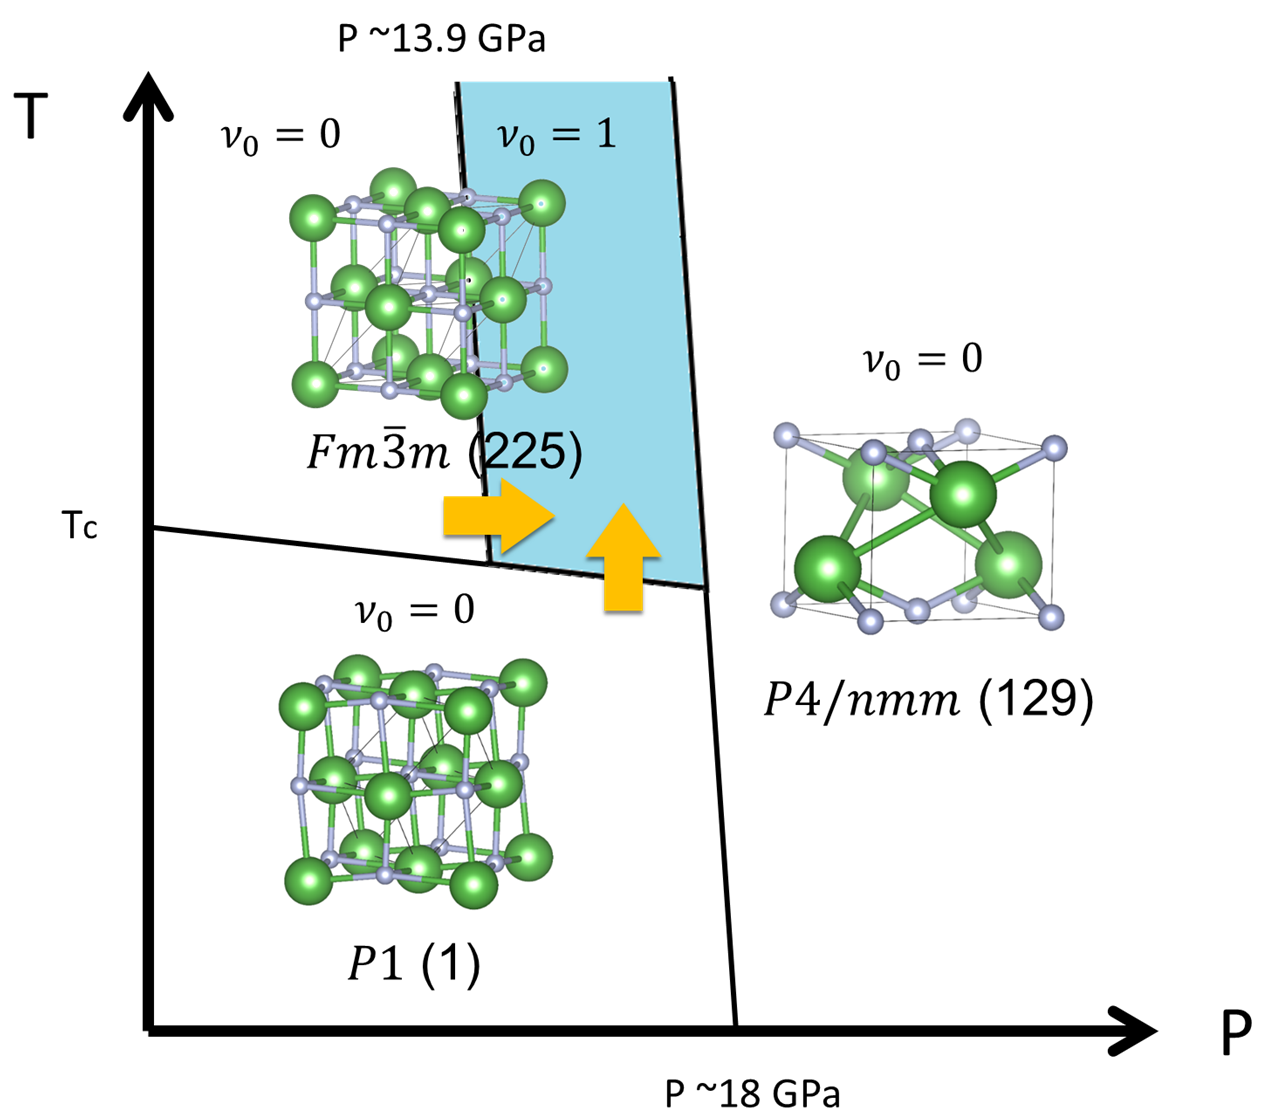
\includegraphics[width=0.8\textwidth]{LaN_phase_diagram.png}
		\caption[Schematic phase diagram of LaN.]{Schematic phase diagram of LaN. The two arrows indicate that the topological phase transition can be driven by either pressure or temperature.}
		\label{fig:LaN_phase_diagram}
	\end{figure*}


	Our study for LaN can be summarized by the schematic phase diagram shown in Fig. \ref{fig:LaN_phase_diagram}. When the pressure and temperature are low, we proposed that LaN has a distorted rock-salt structure ($P1$ symmetry) with spontaneous polarization. Under low temperature, LaN has a pressure-induced structural phase transition from $P1$ structure to $P4/nmm$ structure. Under low pressure, DFT predicts concurrent temperature-induced structural phase transition and ferroelectric transition. Besides, based on our study for topological phase transition, rock-salt LaN becomes topologically non-trivial when the pressure is between 13.9 and 18 GPa. Therefore, based on the phase diagram, the topological phase transition can be achieved by both pressure and temperature as indicated by the arrows in Fig. \ref{fig:LaN_phase_diagram}.



	
		%A tensile strain normally separates valence band and conduction band. Here in LaBi, a tensile strain can restore the normal band ordering, and thus a topological phase transition from nontrivial to trivial. Figure 4 shows the evolution of band structure of LaBi under equal, triaxial, tensile extension. The left hand side is the non-trivial band structure before strain. The inset shows an energy gap = 17 meV at $\Sigma$ because of SOC. When the tensile strain $\varepsilon$ = +2.2\%, the valence band and conduction band meet at $X$, which is a critical point of $\mathbb{Z}_2$ phase transition (also known as a Dirac semimetal phase). When $\varepsilon$ is greater than +2.2\%, the normal band ordering is achieved, and thus the strong index $\nu_0$ become 0. For example, a trivial band structure with $\varepsilon$ = 3.0\% is shown on the right of figure. 4.



	
	\begin{figure*}[ht!]
		\centering
        \captionsetup{singlelinecheck = false, justification=justified}
		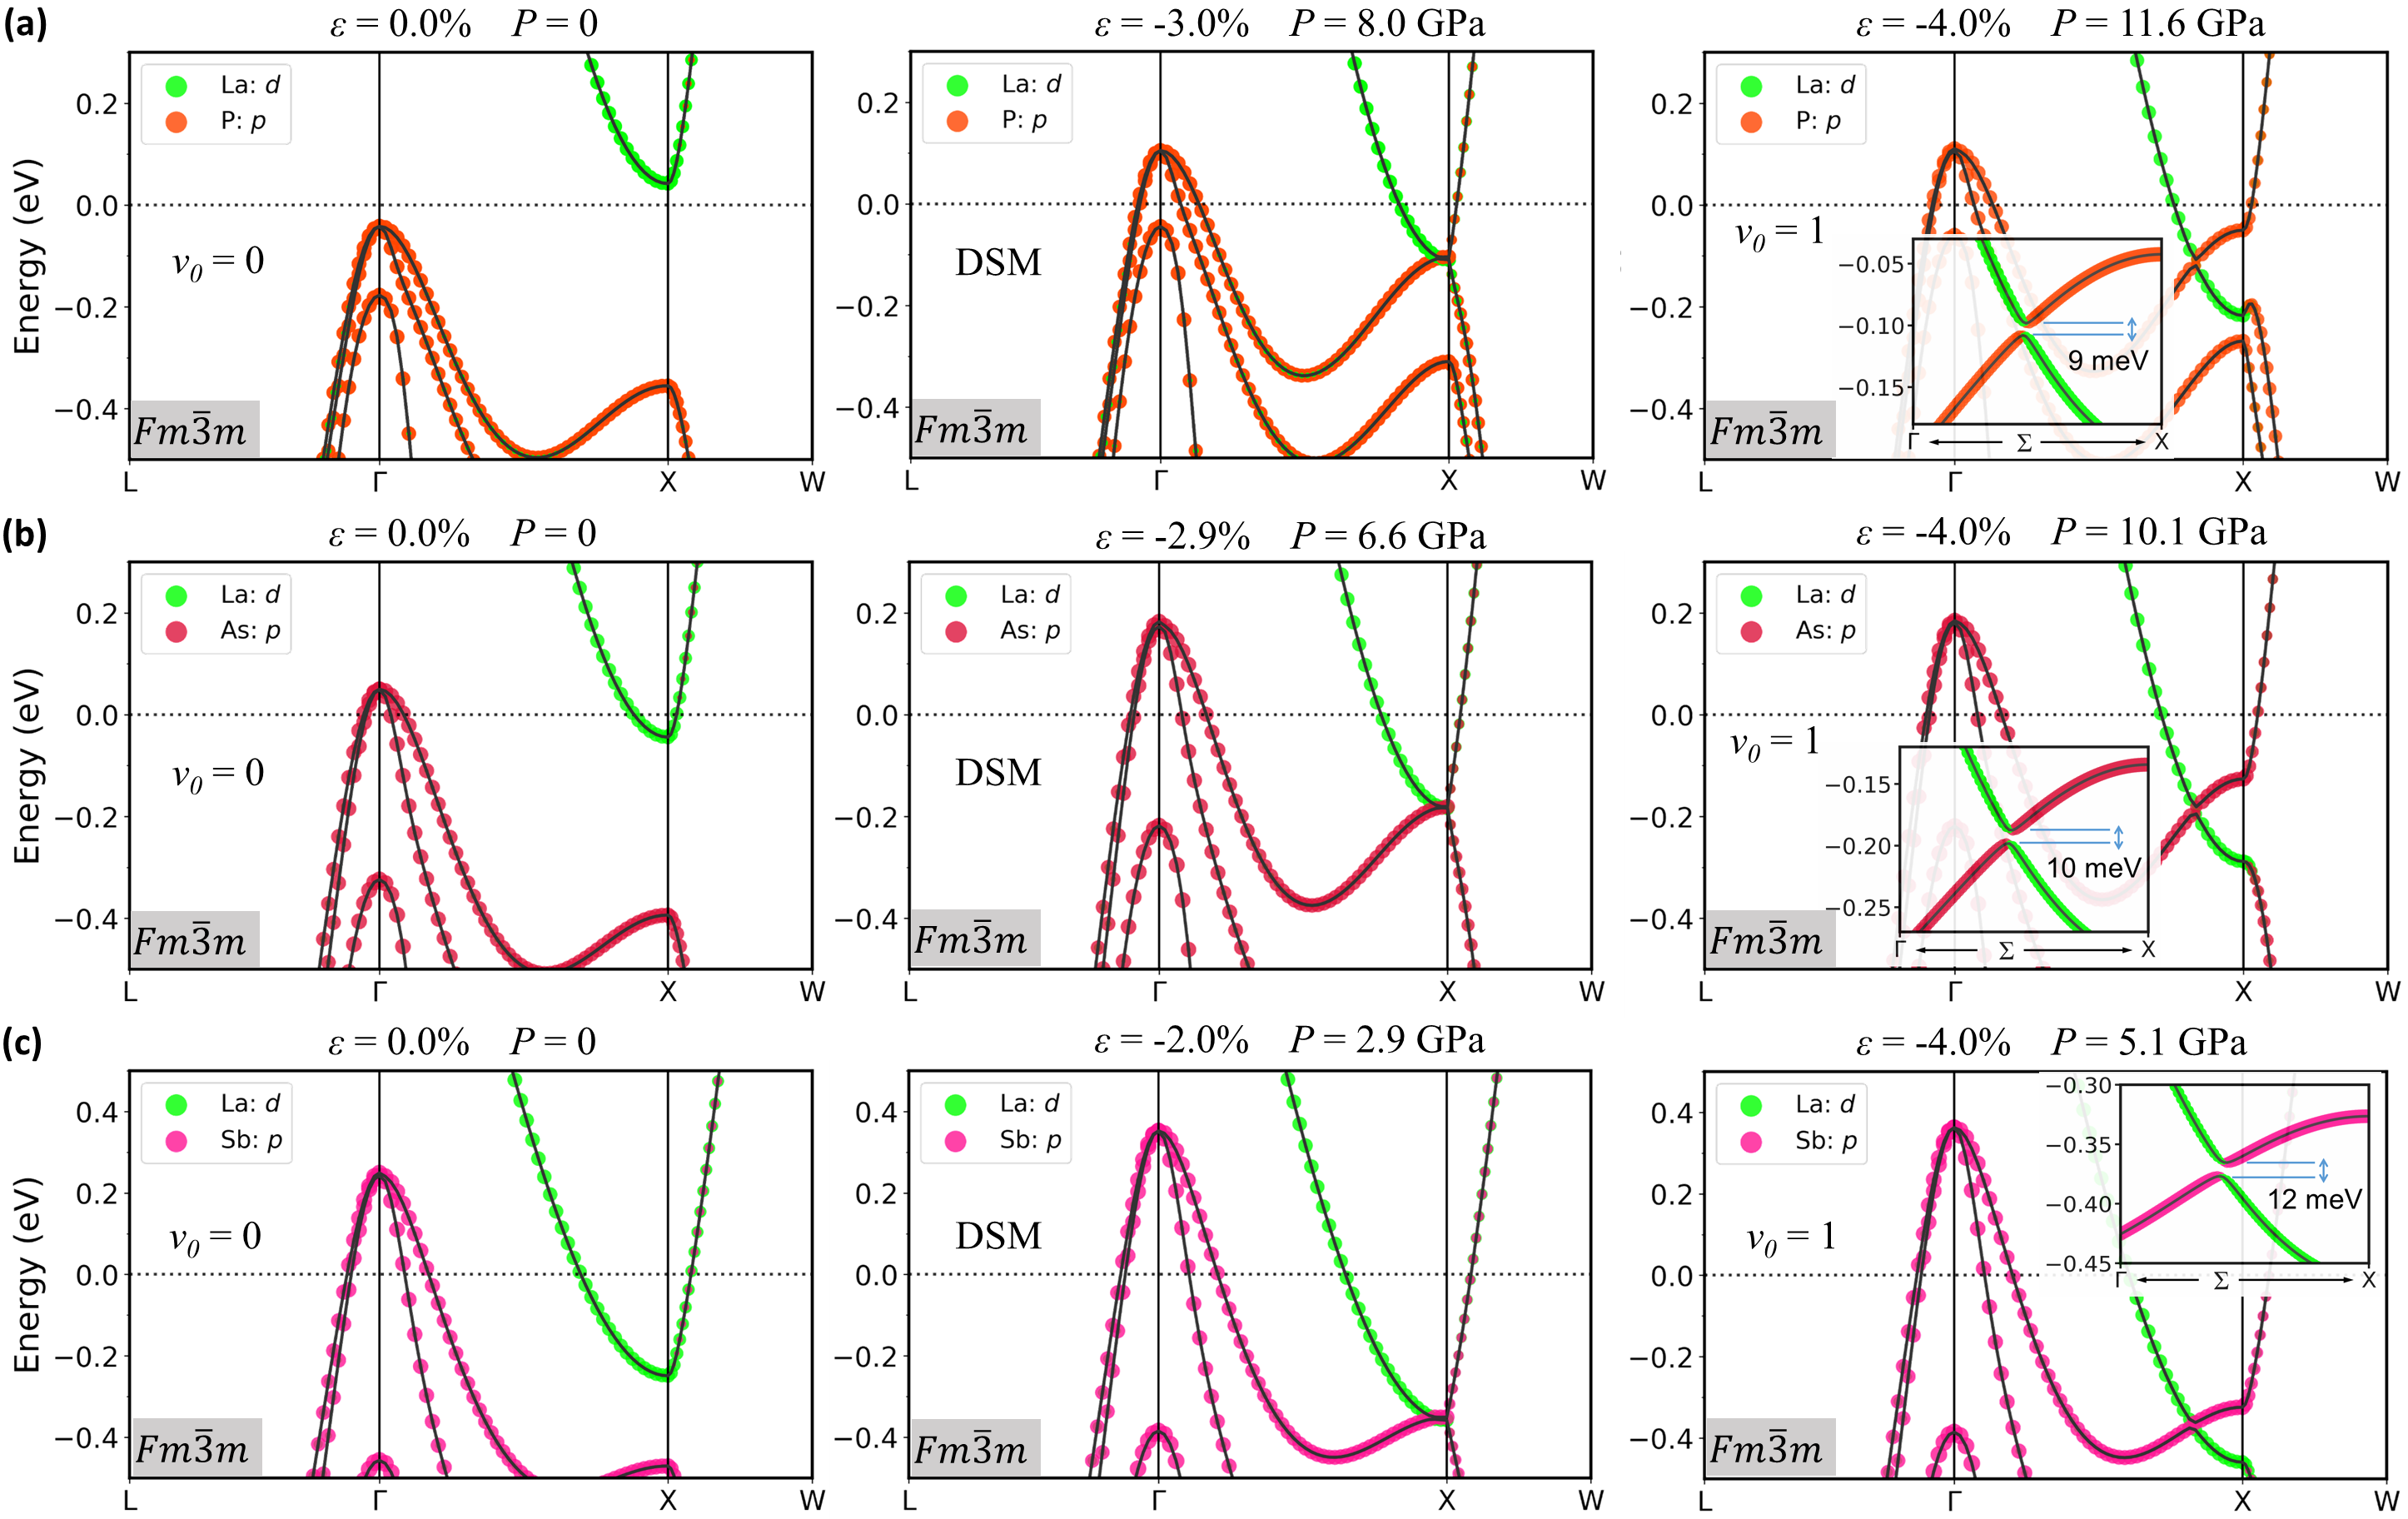
\includegraphics[width=\textwidth]{LaN_8.png}
		\caption[Topological phase transition driven by hydrostatic pressure in rock-salt LaP, LaAs, and LaSb]{
		Electronic band structures and $\mathbb{Z}_2$ topological indices of rock-salt (a) LaP, (b) LaAs, and (c) LaSb, under different strain $\varepsilon$ and corresponding pressure $P$. Left: Trivial insulator ($\nu_0$ = 0). Middle: Dirac semimetal (DSM). Right: Strong topological insulator ($\nu_0$ = 1). The results show pressure-driven topological transitions in rock-salt lanthanum monipnictides..
		}
		\label{fig:LaN_8}
	\end{figure*}
	
	
	Beside the topological phase transition of LaN, we also study pressure-induced topological phase transitions in rock-salt LaP, LaAs, and LaSb, by using a hybrid density functional. The electronic band structures of unstrained LaP, LaAs, and LaSb are shown in the left panels of Fig. \ref{fig:LaN_8}, and they are all found to be topologically trivial ($\nu_0 = 0$) at zero pressure $P=0$. The middle panels of Fig. \ref{fig:LaN_8} show the band structures of LaP, LaAs, and LaSb at the topological transition (Dirac semimetal), where the critical hydrostatic pressures are $P = 8.0$ GPa (with strain value $\varepsilon$ = -3.0\%), 6.6 GPa ($\varepsilon$ = -2.9\%), and 2.9 GPa ($\varepsilon$ = -2.0\%), respectively. Finally, the right panels of Fig. \ref{fig:LaN_8} display the high-pressure band structures, showing band gaps at the $\Sigma$ point with gap sizes of 9, 10, and 12 meV, respectively for LaP, LaAs, and LaSb. This increasing gap size is expected with an increasing spin-orbital coupling strength as one goes down along the periodic table.


	%\section{\label{sec:level1}Conclusion}
	To conclude, using density functional theory and evolutionary crystal searches, we have discovered a new, low-temperature structure of LaN belonging to space group No. 1 with the $P1$ symmetry. This lower-symmetry phase, which can be regarded as a distorted rock-salt structure, displays ferroelectricity with a spontaneous polarization of 36 $\mu$C/cm$^2$. Using {\it ab initio} molecular dynamics, we found that when the temperature is increased, the $P1$-LaN will undergo simultaneous ferroelectric and structural transitions to the more symmetric rock-salt structure (space group 225, $Fm\bar{3}m$). In our enthalpy calculations, $P1$-LaN also could undergo a pressure-induced phase transition to the PbO-like $P4/nmm$ tetragonal structure, when the external pressure is above 18 GPa. In our study of topological properties, the high-temperature rock-salt phase of LaN was found to undergo a pressure-induced transition from a trivial insulator to a strong topological insulator near 13.9 GPa. By increasing the temperature, we also have predicted another topological and structural transition from $P1$-LaN to rock-salt LaN, when the pressure is between 13.9 and $\sim 18$ GPa. These results demonstrate that LaN exhibits a rich phase diagram containing different ferroelectric, structural, and topological phases, and lanthanum monopnictides are intriguing quantum materials that can serve as a platform for exploring novel phase transitions induced by temperature and pressure.

    \vspace{12pt}

    \noindent This section is based on our manuscript on arXiv: arXiv:2104.12879 (2021) \cite{chen2021lan}.






	\pagebreak





    

	

    %\chapter{5 CONCLUSION}
    \addtocounter{numch}{1}
    \addcontentsline{toc}{chapter}{\hspace{4pt}  \the\value{numch} \hspace{4pt} CONCLUSION}
	
	{\centering
		\vspace{0pt} \hspace{0pt} \par
	}
	{\centering
		\vspace{56pt} CHAPTER  \the\value{numch}
	}
	{\centering\singlespacing
		CONCLUSION
	    \par
	}
	{\centering
		\vspace{0pt} \hspace{0pt} \par
	}
	
In the first part of our studies, we focused on computational prediction for new superhard materials using machine learning, evolutionary algorithm, and density functional theory. We studied both B-C-N and B-N-O ternary compounds. For B-C-N materials, we first built machine learning models using existing online database, Materials Project. The models were then used to map out mechanical properties including bulk modulus, shear modulus and hardness. Our machine learning prediction showed that several B-C-N compounds with nearly 1:1 B-N ratio possess superhard property. Following the machine learning prediction, we conducted a series of evolutionary algorithm searches for B-C-N superhard compounds. Our results indicated that BC$_{10}$N has an extremely high hardness $\sim$ 87 GPa. As for B-N-O materials, we generated our own machine learning data by evolutionary searches, and then we adopted a self-improving process to gradually locate the composition of superhard B-N-O compounds. We found that compositions with the formula B$_{x+2}$N$_{x}$O$_{3}$ are superhard and also thermodynamically more stable based on their formation energy and cohesive energy. Our studies of ternary superhard materials show that machine learning can efficiently accelerate the discovery of new functional materials.

Another part of this dissertation is topological materials, we found that ZrTe$_5$ has an extremely small bandgap $\sim$ 60 meV, and it is in the vicinity of topological phase transition. By applying uniaxial strain along $a$-axis, ZrTe$_5$ undergoes a $Z_2$ topological phase transition from a strong topological insulator phase to a weak TI phase. In the case of LaN, we first discovered that the phonon dispersion of LaN is dynamically unstalbe at 0 K, and we found a dynamically stable, low-temperature phase with $P1$ symmetry using evolutionary search. We next study the structural and topological phase transitions in LaN. We found LaN has a structural phase transition to rock-salt phase ($Fm\bar{3}m$ symmetry) when temperature is increased. By studying its phase diagram, our results indicate that high-temperature rock-salt LaN has a normal insulator to a strong topological insulator phase transition at $P$ $\sim$ 14 GPa, and its $Z_2$ transition can also be driven by temperature at $P$ around 14 - 18 GPa. These results indicate that the control of topological phase transition can be effectively achieved by means of strain engineering and the hydrostatic pressure.
	

	\pagebreak
	
    % List of Publications

    \addcontentsline{toc}{chapter}{LIST OF PUBLICATIONS}
	
	{\centering
		\vspace{0pt} \hspace{0pt} \par
	}
	{\centering
		\vspace{56pt} LIST OF PUBLICATIONS
	}
	{\centering\singlespacing
		
	    \par
	}
	{\centering
		\vspace{0pt} \hspace{0pt} \par
	}	
	\noindent Wei-Chih Chen, Joanna N. Schmidt, Da Yan, Yogesh K. Vohra, and Cheng-Chien Chen, “Machine Learning and Evolutionary Prediction of Superhard B-C-N Compounds”, {\it npj Comput Mater} {\bf 7}, 114 (2021).
	
	\vspace{12pt}

    \noindent Wei-Chih Chen, Chia-Min Lin, Joseph Maciejko, and Cheng-Chien Chen, “Structural and Topological Phase Transitions in LaN Driven by Pressure and temperature”, arXiv:2104.12879 (2021).

	\vspace{12pt}
	
	\noindent Chia-Min Lin, Wei-Chih Chen, and Cheng-Chien Chen, “First-Principles Study of Strain Effect on Thermoelectric Properties of LaP and LaAs”, arXiv:2008.06455 (2020).

	\vspace{12pt}

	\noindent Kaleb Burrage, Chia-Min Lin, Wei-Chih Chen, Cheng-Chien Chen, and Yogesh K. Vohra, “Electronic structure and anisotropic compression of Os$_2$B$_3$ to 358 GPa”, {\it J. Condens. Matter Phys.} {\bf 32}, 405703 (2020).
	
	\vspace{12pt}
	
    \noindent Kallol Chakrabarty, Wei-Chih Chen, Paul A. Baker, Vineeth M. Vijayan, Cheng-Chien Chen, and Shane A. Catledge, “Superhard Boron-Rich Boron Carbide with Controlled Degree of Crystallinity”, {\it Materials} {\bf 13}, 3622 (2020).
    
	\vspace{12pt}
    
    \noindent Paul A. Baker, Wei-Chih Chen, Cheng-Chien Chen, Shane A. Catledge, and Yogesh K. Vohra, “First-Principles Predictions and Synthesis of B$_{50}$C$_2$ by Chemical Vapor Deposition”, {\it Sci. Rep.} {\bf 10}, 4454 (2020).

	\vspace{24pt}
    
    \noindent Kaleb Burrage, Chia-Min Lin, Wei-Chih Chen, Cheng-Chien Chen, and Yogesh K. Vohra, “Experimental and Computational Studies on Superhard Material Rhenium Diboride to Ultrahigh Pressures”, {\it Materials} {\bf 13}, 1657 (2020).
 	
 	\vspace{12pt}
 	
    \noindent Bijuan Chen, Ekaterina M. Pärschke, Wei-Chih Chen, Brandon Scoggins, Bing Li, Mahalingam Balasubramanian, Steve Heald, Jianbo Zhang, Hongshan Deng, \newline Raimundas Sereika, Yesudhas Sorb, Xia Yin, Yan Bi, Ke Jin, Qiang Wu, Cheng-Chien Chen, Yang Ding, and Ho-kwang Mao “Probing Cerium 4f States across the Volume Collapse Transition by X‑ray Raman Scattering”, {\it J. Phys. Chem. Lett.} {\bf 10},  7890 (2019).

 	\vspace{12pt}

    \noindent Joshua Mutch, Wei-Chih Chen, Preston Went, Tiema Qian, Ilham Zaky Wilson, Anton Andreev, Cheng-Chien Chen, and Jiun-Haw Chu, “Evidence for a strain tuned topological phase transition in ZrTe$_5$”, {\it Sci. Adv.} {\bf 5}, eaav9771 (2019).
    
 	\vspace{12pt}

    \noindent Paul A. Baker, Shane A. Catledge, Sumner B. Harris, Kathryn J. Ham, Wei-Chih Chen, Cheng-Chien Chen, and Yogesh K. Vohra, “Computational Predictions and Microwave Plasma Synthesis of Superhard Boron-Carbon Materials”, {\it Materials} {\bf 11}, 1279 (2018).

	

	
	
	
	\pagebreak

	{\centering
		\vspace{0pt} \hspace{0pt} \par
	}
	{\centering
		\vspace{24pt} \hspace{0pt} \par
	}
	\hfill  REFERENCES { } { } \hfill
	{\centering
		\vspace{0.2in} \hspace{0pt} \par
	}
	
    \addcontentsline{toc}{chapter}{REFERENCES}
    \bibliographystyle{unsrt}
%    \bibliographystyle{phys}
%    \bibliographystyle{abbrv}
    \bibliography{bibfile.bib}

    %\pagebreak
    %for testing: \gls{HV}
\end{document}